\documentclass{../thunote}

\theoremstyle{definition}
\newtheorem*{corollary}{推论}
\newtheorem*{remark}{注}
\newtheorem*{lemma}{引理}

\newcommand*{\qqquad}{\qquad\quad}
\newcommand*{\qqqquad}{\qquad\qquad}

\let\geq\geqslant
\let\leq\leqslant
\newcommand*{\avg}[1]{\overline{#1}}
\newcommand*{\vs}{~\text{-}~}
\newcommand{\fracdisp}[2]{\frac{\displaystyle #1}{\displaystyle #2}}

% 正体符号
\newcommand*{\const}{\mathrm{const}}
\newcommand*{\plusc}{{\color{lightgray}\,+\,\const}}
\newcommand*{\e}{\mathop{}\!\mathrm{e}^}  % exp
\let\accenti\i
\renewcommand*{\i}{\mathrm{i}}
\newcommand*{\D}{\Delta}
\newcommand*{\p}{\partial}

\usepackage{bm}
\newcommand{\hatbm}[1]{\hat{\bm{#1}}}  % bm with hat, maybe Fourier Transform
\newcommand{\nvec}[1]{\hat{\bm{#1}}}  % normalized vector, without space
\newcommand{\uvec}[1]{\mathop{}\!\nvec{#1}}  % unit vector, with possible space
\newcommand{\dotbm}[1]{\dot{\bm{#1}}}

\usepackage{mathrsfs}  % \mathscr
% \usepackage{boondox-cal}  % \mathcal

\newcommand*{\RR}{\mathbb R}
\newcommand*{\CC}{\mathbb C}
\newcommand*{\ZZ}{\mathbb Z}
\newcommand*{\NN}{\mathbb N}

% \newcommand*{\cL}{\mathcal L}  % linear operator
% \newcommand{\cl}[1]{\mathcal L\fkh{#1}}
% \newcommand{\cli}[1]{\mathcal L^{-1}\!\fkh{#1}}
% \newcommand{\cf}[2][{}]{\mathcal F_{\mathrm{#1}}\fkh{#2}}
% \newcommand{\cfi}[2][{}]{\mathcal F_{\mathrm{#1}}^{-1}\!\fkh{#2}}

\usepackage{cancel}% 删除线

\usepackage{xfrac}

% \usepackage{emoji}  % LuaTeX needed

% 导数等
\let\divides\div
\renewcommand*{\div}{\nabla\cdot}
\newcommand*{\curl}{\nabla\times}

\let\accentd\d
\renewcommand*{\d}{\mathop{}\!\mathrm{d}}
\newcommand*{\nd}{\mathrm{d}}
\newcommand*{\vd}{\mathop{}\!\delta}  % δ
\newcommand{\dd}[2][{}]{\frac{\nd^{#1}}{\nd{#2}^{#1}}}  % d/dx我知道 \,\! 很愚蠢,但是 {} 无法在 Math Preview 上预览
% \newcommand{\dn}[2]{\frac{\nd^{#1}}{\nd #2^{#1}}}  % d^n/dx^n\dn2x≡\dd[2]x
\newcommand{\dv}[3][{}]{\frac{\nd^{#1}#2}{\nd{#3}^{#1}}}  % df/dx
% \newcommand{\du}[3]{\frac{\nd^{#1}#2}{\nd #3^{#1}}}  % d^nf/dx^n\du2fx≡\dv[2]fx
\newcommand{\pp}[2][{}]{\frac{\p^{#1}}{\p{#2}^{#1}}}  % ∂/∂x
% \newcommand{\pn}[2]{\frac{\p^{#1}}{\p #2^{#1}}}  % ∂^n/∂x^n\pn2x≡\pp[2]x
\newcommand{\pv}[3][{}]{\frac{\p^{#1}#2}{\p{#3}^{#1}}}  % ∂f/∂x
% \newcommand{\pu}[3]{\frac{\p^{#1}#2}{\p #3^{#1}}}  % ∂^nf/∂x^n\pu2x≡\pv[2]x
\newcommand{\pw}[3]{\frac{\p^2{#1}}{\p{#2}\p{#3}}}  % ∂^2f/∂x∂y
\newcommand{\dvd}[2]{\left.{#1}\middle/{#2}\right.}

% 积分
\newcommand*{\zti}{_0^{+\infty}}
\newcommand*{\iti}{_{-\infty}^{+\infty}}
\newcommand*{\toinf}{{\to\infty}}

% \newcommand{\ud}[2]{^{#1}{}_{#2}}
% \newcommand{\du}[2]{_{#1}{}^{#2}}

% 括号
\newcommand{\abs}[1]{\left\lvert#1\right\rvert}% |x| 绝对值
\newcommand{\norm}[1]{\left\lVert#1\right\rVert}% ||x|| 模
\newcommand{\edg}[1]{\left.#1\right\rvert}% f|  竖线
\newcommand{\kh}[1]{\left(#1\right)}% (x) 括号
\newcommand{\bigkh}[1]{\bigl(#1\bigr)}
\newcommand{\Bigkh}[1]{\Bigl(#1\Bigr)}
\newcommand{\biggkh}[1]{\biggl(#1\biggr)}
\newcommand{\fkh}[1]{\left[#1\right]}% [x] 方括号
\newcommand{\bigfkh}[1]{\bigl[#1\bigr]}
\newcommand{\Bigfkh}[1]{\Bigl[#1\Bigr]}
\newcommand{\biggfkh}[1]{\biggl[#1\biggr]}
\newcommand{\hkh}[1]{\left\{#1\right\}}% {x} 花括号
\newcommand{\floor}[1]{\left\lfloor#1\right\rfloor}
\newcommand{\ceil}[1]{\left\lceil#1\right\rceil}
\newcommand{\set}[2]{\left\{#1\,\middle\vert\,#2\right\}}% {x|x1,x2,...} 集合
\newcommand{\ave}[1]{\left\langle #1\right\rangle}% <x> 平均值
\newcommand{\bra}[1]{\left\langle #1\right\vert}% <ψ| 左矢
\newcommand{\ket}[1]{\left\vert #1\right\rangle}% |ψ> 右矢
\newcommand{\brkt}[2]{\left\langle #1\middle\vert #2\right\rangle}% <φ|ψ> 内积
\newcommand{\ktbr}[2]{\left\vert#1\right\rangle\hspace{-3pt}\left\langle #2\right\vert}% |ψ><φ|
% \newcommand{\inp}[2]{\left\langle #1,#2\right\rangle}% <f,g> 内积

\newcommand{\nnorm}[1]{\lVert#1\rVert}
\newcommand{\nset}[2]{\{#1\,|\,#2\}}

% 数学运算符
\let\Real\Re
\let\Imaginary\Im
\let\Re\relax
\let\Im\relax
\DeclareMathOperator{\Re}{Re}  % real part
\DeclareMathOperator{\Im}{Im}  % imaginary part
\DeclareMathOperator{\sech}{sech}
\DeclareMathOperator{\csch}{csch} 
\DeclareMathOperator{\arcsec}{arcsec}
\DeclareMathOperator{\arccot}{arccot} 
\DeclareMathOperator{\arccsc}{arccsc} 
\DeclareMathOperator{\arsinh}{arsinh} 
\DeclareMathOperator{\arcosh}{arcosh} 
\DeclareMathOperator{\artanh}{artanh} 
\DeclareMathOperator{\sgn}{sgn}  % 符号函数
\DeclareMathOperator{\Li}{Li}% 
\DeclareMathOperator{\Si}{Si}
\DeclareMathOperator{\Ci}{Ci}
\DeclareMathOperator{\sinc}{sinc}
\DeclareMathOperator{\Heaviside}{H}
\DeclareMathOperator{\arr}{A}% 排列数
\DeclareMathOperator{\com}{C}% 组合数
\DeclareMathOperator{\Res}{Res}% 留数
\DeclareMathOperator{\supp}{supp}% 支撑集
\DeclareMathOperator{\Int}{Int}% 内部
\DeclareMathOperator{\Ext}{Ext}% 外部
\newcommand*{\bigo}{\mathcal O}
\newcommand*{\degree}{^\circ}

% 线性代数
\DeclareMathOperator{\rank}{rank}
\DeclareMathOperator{\id}{id}
\DeclareMathOperator{\diag}{diag}
\newcommand*{\tp}{^\top}  % A^T 转置
\newcommand*{\cj}{^\ast}  % A^* 共轭
\newcommand*{\dg}{^\dagger}  % A^† 共轭转置
\newcommand*{\iv}{^{-1}}  % A^-1

% 物理学家
\newcommand*{\Schr}{Schrödinger}
\newcommand*{\Legd}{Legendre}
\newcommand*{\deB}{de Broglie}
\newcommand*{\Rayl}{Rayleigh}
\newcommand*{\Lande}{Landé}

% 粒子
\newcommand*{\elc}{\mathrm e}
\newcommand*{\pton}{\mathrm p}
\newcommand*{\nton}{\mathrm n}
\newcommand*{\mol}{\mathrm m}

% 物理常数
\newcommand*{\NA}{N_{\mathrm A}}% Avogadro 常数
\newcommand*{\kB}{k_{\mathrm B}}% Boltzmann 常数
\newcommand*{\muB}{\mu_\mathrm B}% Bohr 磁矩

% 
\newcommand*{\Ek}{E_{\mathrm k}}% 动能
\newcommand*{\eff}{_\mathrm{eff}}% 有效下标
\newcommand*{\tot}{_\mathrm{tot}}
\newcommand*{\maxi}{_\mathrm{max}}
\newcommand*{\mini}{_\mathrm{min}}
\newcommand*{\lSI}{\tag{SI}}
\newcommand*{\CGS}{\tag{CGS}}% cm, g, s 制
\newcommand*{\FWHM}{\mathrm{FWHM}}


\newenvironment{equationset}{\left\{\begin{aligned}}{\end{aligned}\right.}

\DeclareMathOperator{\cof}{cof} % cofactor matrix
\let\oldC\C
\let\C\relax
\DeclareMathOperator{\C}{C}     % column space
\DeclareMathOperator{\N}{N}     % null space
\DeclareMathOperator{\rref}{rref}   % reduce row echelon form
\DeclareMathOperator{\lspan}{span}  % linear span
\DeclareMathOperator{\adj}{adj}     % adjuate
\DeclareMathOperator{\im}{im}       % image of mapping
\DeclareMathOperator{\ord}{ord}     % order
\DeclareMathOperator{\sym}{sym}     % symmetric
\DeclareMathOperator{\GL}{GL}  % general linear
\DeclareMathOperator{\SL}{SL}  % special linear

\begin{document}

\title{线性代数\\Linear Algebra}
\maketitle

\frontmatter
\tableofcontents

\mainmatter
\chapter{运动学}

本章主要讨论质点和质点系统的运动学(kinematics)。
运动学描述系统(点、物体、点的系统等等)的运动,而不关心系统为什么会这么运动(这是动力学的内容)。

\section{Galileo时空}

\subsection{仿射空间}

基于Galileo相对性原理,我们需要研究一个“去掉原点的线性空间”。
\begin{definition}{仿射空间}{affine space}
    一个仿射空间(affine space) $(A,V)$是一个集合$A$和一个与之相伴的线性空间$V$。且存在映射
    \begin{equation}
        f:A\times V\to A:(a,v)\mapsto a+v,
    \end{equation}
    满足:
    \begin{itemize}
        \item 右幺(right identity):$V$中的零向量0满足$\forall a\in A$有$a+0=a$;
        \item 结合律(associativity):$\forall u,v\in V,\forall a\in A$有$(a+u)+v=a+(u+v)$;
        \item 正则性:$\forall a\in A$,映射$V\to A:v\mapsto a+v$是一个双射。
    \end{itemize}
    % 仿射空间$(A,V)$的维数就是相伴线性空间$V$的维数$\dim(V)$。
\end{definition}
\begin{remark}~
    \begin{itemize}
        \item 仿射空间与线性空间的区别在于其没有原点,所以仿射空间没有定义加法;
        \item 前两个性质定义了$V$作为加法群在$A$上的右作用,正则性等价于这个作用具有:
        \begin{itemize}
            \item 传递性(transitive):$\forall a,b\in A,\exists v\in V$使得$b=a+v$;
            \item 自由(free):$u,v\in V$,如果存在$a\in A$使得$a+u=a+v$,则$u=v$;
        \end{itemize}
        \item $\forall v\in V$,$v$在$A$上的右作用可定义映射:
        \[
            g_v:A\to A:a\mapsto a+v
        \]
        $g_v$是一个双射,称为$A$上的一个平移(translation),故$V$也叫$A$的平移空间;
        \item 减法:$\forall a,b\in A$,存在唯一的$v\in V$使得$b=a+v$。记$v=b-a$。
    \end{itemize}
\end{remark}
\begin{example}{}{}
    $V$是一个线性空间,则$(V,V)$是一个仿射空间,其右作用就是线性空间的加法。

    $V$是$\RR^n$中一个$m$维的线性子空间,$v\in\RR^n$,则$(V+v,V)$是一个仿射空间。
\end{example}

后面我们用$\AA^n$表示平移空间为$\RR^n$的$n$维仿射空间。

\begin{definition}{仿射标架}{affine frame}
    仿射空间$(A,V)$的仿射标架(affine frame)是集合$\{o;v_1,\ldots,v_n\}$,其中$o\in A$是原点(origin),$(v_1,\ldots,v_n)$是$V$的一组基。由定义,$\forall a\in A$都可以被唯一地写成
    \begin{equation}
        a=o+\lambda^1v_1+\cdots+\lambda^nv_n,
    \end{equation}
    $(\lambda^1,\ldots,\lambda^n)$是$a$在仿射标架$\{o;v_1,\ldots,v_n\}$中的仿射坐标(affine coordinates)。
\end{definition}
仿射标架定义了一一映射$A\to\RR^n:a\mapsto(\lambda^1,\ldots,\lambda^n)$

\subsection{Galileo时空}

经典力学的时空模型是Galileo时空。

\begin{definition}{Galileo时空}{Galilean spacetime}
    Galileo时空(spacetime)是一个拥有Galileo结构(structure)的四维仿射空间$(\AA^4,\RR^4)$:
    % $a\in\AA^4$称为事件(event)或世界点(world point)。
    \begin{itemize}
        \item 时间$T$是非零线性映射$T:\RR^4\to\RR$。
        
        $\forall a,b\in\AA^4$,事件$a$和事件$b$的时间间隔为$T(b-a)$;
        \item 若$T(b-a)=0$,则$a$和$b$是同时的(simultaneous)。
        
        事件$a$的同时空间是$\AA_a=\{b\in\AA^4\,|\,T(b-a)=0\}$,同构于$\AA^3$;
        \item $\forall a,b\in\AA_c$,同时事件$a,b$之间的距离定义为
        \begin{equation}
            d(a,b)\equiv|a-b|=\sqrt{(a-b,a-b)},
        \end{equation}
        其中$(\cdot,\cdot)$是$\RR^3$中的Euclid内积。即每个同时空间$\AA_c$相伴的平移空间是一个Euclid空间。
    \end{itemize}
\end{definition}
\begin{example}{Galielo坐标时空}{Galilean coordinate spacetime}
    考虑$\RR\times\RR^3$作为仿射空间,并在$\RR^3$的平移空间上赋予通常的Euclid度量,则$\RR\times\RR^3$是一个Galileo时空,也记为$\RR_t\times\RR^3$。时间$T$为投影映射
    \begin{equation}
        \pi_t:\RR_t\times\RR^3\to\RR_t:(t,\bm x)\mapsto t.
    \end{equation}
    这个仿射空间也叫Galielo坐标时空。
\end{example}
\begin{definition}{Galileo群}{Galilean group}
    Galileo群$\Gal(3)$是$\AA^4$上所有保持Galileo结构的仿射变换构成的群。即$\forall g\in\Gal(3)$:
    \begin{itemize}
        \item $\forall a,b\in\AA^4,T(g(a)-g(b))=T(a-b)$;
        \item $\forall a,b\in\AA_c,d(g(a),g(b))=d(a,b)$;
    \end{itemize}
\end{definition}
\begin{theorem}{}{}
    $\RR\times\RR^3$上的Galileo群$\Gal(3)$由以下三类变换的复合生成:
    \begin{itemize}
        \item 匀速运动$g_1:(t,\bm x)\mapsto(t,\bm x+\bm vt)$,其中速度$\bm v\in\RR^3$;
        \item 平移$g_2:(t,\bm x)\mapsto(t+s,\bm x+\bm s)$,其中$(s,\bm s)\in\RR\times\RR^3$;
        \item 转动$g_3:(t,\bm x)\mapsto(t,S\bm x)$,其中$S\in O(3)$
    \end{itemize}
    $\forall g\in\Gal(3)$都可以被唯一地写成$g=g_1\circ g_2\circ g_3$。
\end{theorem}
\begin{example}{}{}
    映射$(t,\bm x)\mapsto(t,\bm x+\bm at^2/2)\notin\Gal(3)$,因为它不是仿射变换。
\end{example}
\begin{theorem}{}{}
    所有Galileo时空都互相同构;特别地,也都同构于Galileo坐标时空$\RR\times\RR^3$。
\end{theorem}
因此如无额外说明,以后提到的Galileo时空都指$\RR\times\RR^3$。

\subsection{Galileo时空中粒子的运动}
当我们不关心对象的内部结构,只关心对象的位置的时候,我们可以用一个点来代表它,称之为粒子(particle)。
\begin{definition}{世界线}{world line}
    Galileo时空中,一个粒子的运动轨迹(trajectory)或世界线(world line)是$\RR_t\times\RR^3$的一个可微\footnote{此处指总是具有所需要的可微性质。}截面$\sigma:\RR_t\to\RR_t\times\RR^3$。

    更一般地,我们可以用可微映射$q:I\to\RR^3$描述单个粒子的运动,其中$I$是$\RR_t$的一个区间。
    % 它也定义了$\RR\times\RR^3$中的一个局部截面。这个轨迹也可以看成是完整轨迹的一部分。
    映射$q$的陪域$\RR^3$也叫做位形空间(configuration space)。

    当位形空间是$\RR^n$的时候,我们也将$q$记为$\bm x$或者$\bm x(t)$。
\end{definition}
伽利略时空中单粒子的位形空间即是$\RR^3$。
\begin{definition}{速度}{velocity}
    若某粒子在Galileo时空中的运动由$\bm x(t)$描述,则$\bm x(t)$的一阶导
    \begin{equation}
        \dotbm x=\dv{\bm x}t,
    \end{equation}
    是速度(velocity)矢量。
\end{definition}
\begin{example}{}{}
    考虑匀速直线运动$\bm x(t)=\bm x_0+\bm vt$,$\dotbm x(t)=\bm v$是一个常映射。
    匀速直线运动在Galileo变换下仍然是匀速直线运动。
\end{example}

\begin{definition}{多粒子运动}{}
    Galileo时空中$N$个粒子的运动可以用$\RR_t\times\RR^3$中的$N$个截面$\sigma_1,\ldots,\sigma_N$描述。但是为了体现经典力学中的绝对时间,即不同粒子的运动共用一个时间轴$\RR_t$,我们应该用
    \[
        \underbrace{(\RR_t\times\RR^3)\times_{\RR_t}\cdots\times_{\RR_t}(\RR_t\times\RR^3)}_N
    \]
    中的一个截面来描述这$N$个粒子的运动轨迹。其中$\times_{\RR_t}$是$\RR_t$上的纤维积(fiber product),其定义为
    \begin{equation}
        (\RR_t\times\RR^3)\times_{\RR_t}(\RR_t\times\RR^3)\equiv\{(t_1,\bm x_1,t_2,\bm x_2)\in(\RR_t\times\RR^3)\times(\RR_t\times\RR^3)\,|\,t_1=t_2\}
    \end{equation}
    等价地,Galileo时空中$N$个粒子的运动可以用映射$\bm x(t):\RR_t\to\RR^{3N}$或$\bm x(t):I\to\RR^{3N}$描述。此时位形空间为$\RR^{3N}$。
\end{definition}

\section{约束系统}

\begin{definition}{约束}{constraints}
    很多时候粒子的位置$\bm x(t)$需要满足额外的方程$f(\bm x)=0$,这些方程叫做对系统的约束(constraints)。
\end{definition}
\begin{example}{球面约束}{constraints, |x|=l}
    考虑一个被限制在半径为$\ell$的球面上的粒子,其坐标$\bm x$满足约束
    \[
        \abs{\bm x}^2=\ell^2,
    \]
    这个约束在变换$(t,\bm x)\mapsto(t,\bm x+\bm vt)$下变成一个与时间$t$相关的约束,因此其与Galileo结构不相容。因为这个约束将球面的球心看作一个特殊的点。
\end{example}
\begin{example}{刚性杆约束}{constraints, |x1-x2|=l}
    考虑被长为$\ell$的刚性杆连接的两个粒子,其坐标$(\bm x_1,\bm x_2)$满足约束
    \[
        \abs{\bm x_1-\bm x_2}^2=\ell^2,
    \]
    这个约束在Galileo变换下始终保持同样的形式,因此其与Galileo结构相容。
\end{example}
当有约束的时候,选取不同的坐标系可能会让约束简化。
\begin{example}{球面约束·续}{constraints, |x|=l, II}
    接\exmref{exm:constraints, |x|=l},约束在直角坐标系下是关于$\bm x=(x,y,z)$三个分量的方程。但若选取球坐标$(r,\theta,\phi)$满足
    \[
        \bm x=(r\sin\theta\cos\phi,r\sin\sin\theta\phi,r\cos\theta)
    \]
    约束$\abs{\bm x}^2=\ell^2$在球坐标下变为
    \[
        \abs r^2=\ell^2,
    \]
    与$\theta,\phi$无关。此时粒子的位形空间为区域$0\leq\theta<\pi$和$0\leq\phi<2\pi$。
\end{example}

\subsection{微分流形}

有约束的系统的位形空间是一个微分流形。

\begin{definition}{拓扑}{}
    集合$X$上的拓扑(topology) $\mathcal T$是$X$的子集族,其元素称为$X$的开集(open set),满足:
    \begin{itemize}
        \item $\varnothing,X$是$X$的开集:$\varnothing\in\mathcal T,X\in\mathcal T$;
        \item 有限个$X$的开集之交是$X$的开集:$\forall U_i\in\mathcal T,\cup_{i=1}^nU_i\in\mathcal T$;
        \item 任意个$X$的开集之并是$X$的开集:$\forall U_i\in\mathcal T,\cap_{i=1}^\infty U_i\in\mathcal T$。
    \end{itemize}
    并称$(X,\mathcal T)$是拓扑空间(topological space)。
\end{definition}
在明确了拓扑$\mathcal T$后,可以只用$X$表示拓扑空间。
\begin{definition}{同胚}{homeomorphic}
    两个拓扑空间$(X,\mathcal T_X)$和$(Y,\mathcal T_Y)$之间的同胚映射(homeomorphism)
    \begin{equation}
        f:(X,\mathcal T_X)\to(Y,\mathcal T_Y)
    \end{equation}
    满足:$f$是一个双射,且$f$和$f^{-1}$是连续的。
    
    此时称$X,Y$是同胚的(homeomorphic)或拓扑同构的(topological isomorphic),记作$X\cong Y$。
\end{definition}
\begin{theorem}{}{}
    同胚是一种等价关系:
    \begin{itemize}
        \item 自反性:$X\cong X$,即任何拓扑空间都与其自身同胚;
        \item 对称性:$X\cong Y\iff Y\cong X$;
        \item 传递性:$X\cong Y,Y\cong Z\implies X\cong Z$。
    \end{itemize}
\end{theorem}
\begin{example}{}{}
    在Euclid度量空间$(\RR,\rho)$中,任何开区间都是同胚的,比如可以找到$(0,1)$与$(1,+\infty)$之间的同胚映射:
    \[
        f:(0,1)\to(1,+\infty):x\mapsto\frac1x.
    \]
    同时,任何闭区间都是同胚的。
\end{example}
\begin{definition}{坐标卡}{coordinate chart}
    一个$n$维的坐标卡(coordinate chart)是拓扑空间$X$中的一个开集$U$到$\RR^n$的开集$V$的同胚映射
    \begin{equation}
        \phi:U\to V\subset\RR^n.
    \end{equation}
    其中$U$和$V$上各自赋予子空间拓扑。
\end{definition}
物理上的坐标系一般指某个坐标卡。我们也将坐标卡记为$(U,\phi)$。
\begin{definition}{连接函数}{transition function}
    若$\phi:U_1\to V_1$和$\psi:U_2\to V_2$是$X$上的两个坐标卡,且$U_1\cap U_2\neq\varnothing$,则$\phi,\psi$之间的连接函数(transition function)为
    \begin{equation}
        \psi\circ\phi^{-1}:\phi(U_1\cap U_2)\mapsto\psi(U_1\cap U_2).
    \end{equation}
    若$\psi\circ\phi^{-1}$可微,则$\phi,\psi$是相容或相关的(compatible)。若$U_1\cap U_2=\varnothing$,则默认相容。
\end{definition}
\begin{definition}{图册}{atlas}
    对于拓扑空间$X$,若存在一族两两相容的坐标卡$\mathcal A=\{U_i\}_{i\in I}$使得$X=\cup_{i\in I}U_i$,则称$\mathcal A$是$X$的一个图册(atlas)。
\end{definition}
\begin{theorem}{图册的等价关系}{}
    $X$上的两个图册$\mathcal A_1,\mathcal A_2$等价当且仅当其并$\mathcal A_1\cup\mathcal A_2$也是$X$上的一个图册。
    % 这是$X$上所有图册的集合的一个等价关系。
\end{theorem}
\begin{definition}{微分流形}{differentiable manifold}
    拓扑空间$X$上的一个微分结构$\mathcal D$是$X$上等价图册的类。$X$和其上微分结构$\mathcal D$构成一个微分流形(differentiable manifold) $M=(X,\mathcal D)$。
\end{definition}
微分结构$\mathcal D$中所有图册的并$\mathcal A_{\mathcal D}=\cup\set{\mathcal A}{\mathcal A\in\mathcal D}$叫做$\mathcal D$的最大图册。如果一个微分结构中图册的连接函数都是$C^r$函数($r$阶导连续),则称相应的微分流形为$C^r$流形。特别地,如果连接函数都是$C^\infty$函数(光滑函数),我们得到$C^\infty$流形(光滑流形)。如果微分流形$M$是连通的,则它的一个图册中的每个坐标卡的维数都相同,此时这个维数也就是$M$的维数。我们考虑的位形空间基本上都是连通流形。
\begin{example}{}{}
    $(A,V)$是一个$n$维仿射空间。选取仿射标架$(o;v_1,\ldots,v_n)$后得到坐标卡
    \[
        \phi:A\to\RR^n:a\mapsto(\lambda^1,\ldots,\lambda^n),
    \]
    此时坐标卡本身构成一个图册。
\end{example}
\begin{example}{}{}
    $\RR^3$中的单位球面$\mathbb S^2$
    \begin{equation}
        x^2+y^2+z^2=1
    \end{equation}
    上的一个开覆盖$U_N\cap U_S$,其中$U_N=\mathbb S^2\backslash\{S=(0,0,-1)\}$和$U_S=\mathbb S^2\backslash\{N=(0,0,1)\}$。可通过球极投影构造如下坐标卡
    \begin{subequations}
        \begin{align}
            \phi_N:U_N\to\RR^2:(x,y,z)&\mapsto\kh{\frac{2x}{1+z},\frac{2y}{1+z},1};\\
            \phi_S:U_S\to\RR^2:(x,y,z)&\mapsto\kh{\frac{2x}{1-z},\frac{2y}{1-z},-1}.
        \end{align}
    \end{subequations}
    其连接函数
    \begin{equation}
        \phi_{NS}\equiv\phi_N\circ\phi_S^{-1}:\RR^2\backslash\{(0,0)\}\to\RR^2\backslash\{(0,0)\}:(X,Y)\mapsto\kh{\frac{2X}{X^2+Y^2},\frac{2Y}{X^2+Y^2}}
    \end{equation}
    是光滑的。这样我们就得到了$\mathbb S^2$上的一个图册,这个图册所属的等价类就是$\mathbb S^2$上的一个光滑结构。
    \tcblower
    我们还可以在$\mathbb S^2$上定义另一个图册,它也包含两个坐标卡
    \begin{subequations}
        \begin{align}
            \phi_1^{-1}:(0,\pi)\times(0,2\pi)\to(\sin\theta\cos\phi,\sin\theta\sin\phi,\cos\theta);\\
            \phi_2^{-1}:(0,\pi)\times(0,2\pi)\to(\sin\theta\sin\phi,\cos\theta,\sin\theta\cos\phi).
        \end{align}
    \end{subequations}
    这两个坐标卡来源于直角坐标变换成球坐标。可以验证它和之前的图册是等价的。
\end{example}



\chapter{Boltzmann分布}
\section{理想气体}
理想气体在常温常压下满足非简并条件:
\[
	\e\alpha\gg 1,
\]
符合半经典分布。%分子运动可分为质心平动和内部运动,两种运动独立
%\varepsilon\tot=\varepsilon_\tl+\varepsilon_\i,\quad\omega\tot=\omega_\tl\omega_\i.
分子运动可分为质心的平动(translation)、分子内部的振动(vibration)和转动(rotation),三者是相互独立的。
\paragraph{质心平动}
$\varepsilon_\tl$准连续
\[
	\varepsilon_\tl=\frac1{2m}\kh{p_x^2+p_y^2+p_z^2}.
\]
由\exmref{exm:Monatomic Molecule},配分函数
\begin{align}\notag
	Z_\tl(\beta,V) & =\int\zti g(\varepsilon)\e{-\beta\varepsilon}\d\varepsilon                                                                      \\
	               & =\frac{2\pi V}{h^3}\kh{2m}^{3/2}\int\zti\sqrt\varepsilon\e{-\beta\varepsilon}\d\varepsilon=V\kh{\frac{2\pi m}{h^2\beta}}^{3/2}.
\end{align}
单原子分子只有质心平动
\[
	N=\e{-\alpha}Z_\tl,\implies\e{\alpha}=\frac VN\kh{\frac{2\pi m\kB T}{h^2}}^{3/2}\gg 1.
\]
说明稀薄、高温、质量大的情况下,满足非简并条件,
\begin{gather}
	E_\tl=-N\pv{\ln Z_\tl}\beta=\frac32N\kB T.\\
	C_V^\tl=\kh{\pv ET}_V=\frac32N\kB.
\end{gather}
物态方程
\begin{align}
	p=\frac N\beta\pv{\ln Z_\tl}V=\frac{N\kB T}V.
\end{align}
熵
\begin{align}\notag
	S_\tl & =N\kB\kh{\ln Z_\tl-\beta\pv{\ln Z_\tl}\beta-\ln N+1}                 \\
	      & =\frac52N\kB+N\kB\ln\fkh{\frac VN\kh{\frac{2\pi m\kB T}{h^2}}^{3/2}}
\end{align}
\paragraph{振动}
考虑一维振动,%取约化质量$\mu$,
有
\[
	\varepsilon_\vb=h\nu\kh{n+\frac12},\quad\omega_\vb=1.
\]
能量间距
\[
	\D\varepsilon_\vb=h\nu\sim\SI{0.1}\electronvolt\gg\SI{0.025}\electronvolt.
\]
因此必须考虑能级的分立性。
定义振动的特征温度
\[
	\theta_\vb:=\frac{\D\varepsilon_\vb}\kB=\frac{h\nu}\kB\sim\SI{e3}\K.
\]
则配分函数
% \[Z_\nu=\sum\omega_\nu(n)\e{-\beta\varepsilon_\nu(n)}.\]
\begin{align}
	Z_\vb=\sum_{n=0}^\infty\e{-(n+1/2)\beta h\nu}=\frac{\e{-\theta_\vb/2T}}{1-\e{-\theta_\vb/T}}=\frac12\csch\kh{\frac{\theta_\vb}{2T}}.
\end{align}

振动内能
\begin{align}
	E_\vb=-N\pv{\ln Z_\vb}\beta=Nh\nu\fkh{\frac12+\underset{\text{激发能}}{\frac{\e{-\beta h\nu}}{1-\e{-\beta h\nu}}}}=:N\avg\varepsilon.
\end{align}
其中$\avg\varepsilon$为单个原子的振动能。

比热
\begin{align}
	C_V^\vb=\kh{\pv{E_\vb}T}_V=N\kB\Einst\!\kh{\frac{\theta_\vb}T},
\end{align}
其中Einstein函数
\[
	\Einst(x):=\frac{x^2\e x}{\kh{\e x-1}^2}.
\]
\begin{compactitem}
	\item 
	低温极限,由
	\[
		x\gg 1,\quad\Einst(x)\simeq x^2\e{-x}\ll 1
	\]
	因此比热
	\begin{align}
		C_V^\vb\simeq N\kB\kh{\frac{\theta_\vb}T}^2\e{-\theta_\vb/T}.
	\end{align}
	相对振动而言,常温属于低温范围,故振动自由度对$C_V$贡献很小。
	\item
	高温极限,能量准连续
	\begin{align*}
		Z_\vb & =\int\zti g(\varepsilon)\e{-\beta\varepsilon}\d\varepsilon=\frac{2\pi}{h\omega}\int\zti\e{-\beta\varepsilon}\d\varepsilon=\frac{2\pi}{\beta h\omega}=\frac T{\theta_\vb}.
	\end{align*}
	内能
	\[
		E_\vb=N\kB T.
	\]
	
	或由低温算得的结果,使$\beta\to0$
	\[
		E_\vb\simeq Nh\nu\kh{\frac12+\frac1{\beta h\nu}}\simeq N\kB T.
	\]
\end{compactitem}
比较有三个自由度$p_x,p_y,p_z$的平动能量$E_\tl=3\kB T/2$和有两个自由度的振动能量$E_\vb=\kB T$,可以总结这样一个规律:
\begin{theorem}{能量均分定理}{Equi-Partition Theorem}
	高温下,能量准连续,能量的每个自由度对能量贡献为$\kB T/2$。
\end{theorem}
\paragraph{转动}
以异核双原子分子\footnote{同核需考虑全同性原理。比如正氢(两个氢核自旋平行) $\ell$为奇数;仲氢(两个氢核自旋反平行) $\ell$为偶数。}为例,
\[
	\varepsilon_\rt=\frac{\hbar^2}{2I}\ell(\ell+1),\quad\omega_\rt=2\ell+1.
\]
转动特征温度
\[
	\theta_\rt=\frac{\hbar^2}{2I\kB}\sim\SI{10}\K.
\]
配分函数并没有显式表达式:
\[
	Z_\rt=\sum_{\ell=0}^\infty(2\ell+1)\e{-\ell(\ell+1)\,\theta_\rt/T}.
\]
\begin{compactitem}
	\item
	高温极限下,能量准连续
	\[
		Z_\rt=\int\zti g(\varepsilon)\e{-\beta\varepsilon}\d\varepsilon=\frac{8\pi^2I}{h^2}\cdot\frac1\beta=\frac T{\theta_\rt}.
	\]
	或由$\theta_\rt/T\ll 1$
	\[
		Z_\rt\simeq\int_0^{+\infty}\e{-\ell(\ell+1)\,\theta_\rt/T}\cdot(2\ell+1)\d\ell=\frac T{\theta_\rt}.
	\]
	能量和比热
	\begin{align}
		E_\rt=N\kB T,\quad C_V^\rt=N\kB.
	\end{align}
	\item 
	低温极限,$\theta_\rt/T\gg 1$,$Z_\rt$的项很快趋于0
	\[
		Z_\rt=1+3\e{-2\theta_\rt/T},
	\]
	能量和比热
	\begin{align}
		E_\rt&=6N\kB\theta_\rt\e{-2\theta_\rt/T},\\
		C_V^\rt&=12N\kB\kh{\frac{\theta_\rt}T}^2\e{-2\theta_\rt/T}.
	\end{align}
\end{compactitem}
原子内部结构(电子、原子核等)的自由度对宏观量(特别是$C_V$)无贡献。因为在稳定性、结合能、能级间距上,从分子、原子到原子核越来越稳定,特征温度越来越高,越来越难以被激发。即,结合的紧密的自由能被冻结了,通常不激发。
\sectionstar{Maxwell速度分布律}
考虑气体分子质心平动
\[
	\varepsilon=\frac1{2m}\kh{p_x^2+p_y^2+p_z^2},\quad \e{-\alpha}=\frac NV\kh{\frac{h^2}{2\pi m\kB T}}^{3/2}.
\]
在体积$V$内,动量在$\d p_x\nd p_y\nd p_z$范围内的分子数为
\[
	\frac V{h^3}\e{-\alpha-\beta\varepsilon}\d p_x\nd p_y\nd p_z=N\kh{\frac1{2\pi m\kB T}}^{3/2}\e{-\beta\kh{p_x^2+p_y^2+p_z^2}/2m}\d p_x\nd p_y\nd p_z.
\]
从而单位体积内,速度在$\d v_x\nd v_y\nd v_z$范围内的分子数为
\begin{align}
	\begin{aligned}
		&f(v_x,v_y,x_z)\d v_x\nd v_y\nd v_z=n\kh{\frac m{2\pi\kB T}}^{3/2}\e{-m\kh{v_x^2+v_y^2+v_z^2}/2\kB T}\d v_x\nd v_y\nd v_z.
	\end{aligned}
\end{align}
上式即\textbf{Maxwell速度分布率},满足
\[
	\int\iti\int\iti\int\iti f(v_x,v_y,x_z)\d v_x\nd v_y\nd v_z=n.
\]
将坐标$(v_x,v_y,v_z)$换为球坐标$(v,\theta,\phi)$,并对$\theta,\phi$直接积分,便得到速率的分布:
\begin{align}
	f(v)\d v=4\pi n\kh{\frac m{2\pi\kB T}}^{3/2}\e{-mv^2/2\kB T}v^2\d v.
\end{align}
最概然速率$v_\mathrm m$
\begin{gather}
	\dd v\kh{\e{-mv^2/2\kB T}v^2}=0,\implies
	v_\mathrm m=\sqrt{\frac{2\kB T}m}.
\end{gather}
平均速率$\avg v$
\begin{align}
	\avg v=\pi n\kh{\frac m{2\pi\kB T}}^{3/2}\int\zti v\e{-mv^2/2\kB T}v^2\d v=\sqrt{\frac{8\kB T}{\pi m}}.
\end{align}
方均根速率$v_\mathrm s$
\begin{align}\notag
	\avg{v^2}&=\pi n\kh{\frac m{2\pi\kB T}}^{3/2}\int\zti v^2\e{-mv^2/2\kB T}v^2\d v=\frac{3\kB T}m;\\
	v_\mathrm s&=\sqrt{\avg{v^2}}=\sqrt{\frac{3\kB T}m}.
\end{align}

单位时间碰撞单位面积器壁上的分子数
\begin{align}\notag
	\Gamma&=\int\iti\int\iti\int\zti f(v_x,v_y,x_z) v_x\d v_x\nd v_y\nd v_z\\
	&=n\kh{\frac m{2\pi\kB T}}^{1/2}\int\zti\e{-mv_x^2/2\kB T}v_x\d v_x=n\kh{\frac{\kB T}{2\pi m}}^{1/2}=\frac14n\avg v.
\end{align}
\section{Einstein模型}
讨论固体晶格振动对$C_V$的贡献。
\paragraph{简谐近似}
晶格间强耦合,当$T$不太高时,振幅小,在平衡位置展开
\iffalse
	\[
	\varPhi(x_1,x_2,\ldots,x_{3N})=\edg\phi_{x_i=0}+\sum\edg{\pv\phi{x_i}}_{x_i=0}x_i+\frac12\sum\edg{\pw\phi{x_i}{x_j}}_{x_j=0}x_ix_j+\cdots
\]
	保留至二次项
	\[
	H=\sum\frac12\dot x_i^2+\sum\frac12C_{ij}x_ix_j+\phi_0,\quad C_{ij}:=\edg{\pw\phi{x_i}{x_j}}_{x_j=0}.
\]
	使用正交变换使其对角化
	\begin{align*}
		xCx\tp=q\Lambda q\tp.
	\end{align*}
\fi
\[
	H=\sum_{i=1}^{3N}\kh{\frac{p_i^2}{2m}+2\pi^2m\nu_i^2q_i^2}+\phi_0,\quad p_i=m\dot q_i.
\]
晶格振动约化为$3N$个独立、可区别的简谐振动。
\paragraph{Einstein模型}$\nu_i=\nu$且
\[
	\varepsilon_n=h\nu\kh{n+\frac12},\quad n=0,1,2,\ldots
\]
和前面理想气体的振动类似,配分函数
\[
	z(\beta)=\sum_{n=0}^\infty\e{-\beta\varepsilon_n}=\frac{\e{-\beta h\nu/2}}{1-\e{-\beta h\nu}}.
\]
能量,注意此处是$3N$
\begin{align*}
	E & =-3N\pv{\ln z(\beta)}\beta                          \\
	  & =3Nh\nu\kh{\frac12+\frac1{\e{\beta h\nu}-1}}+\phi_0
	=\frac{3Nh\nu}{\e{\beta h\nu}-1}+E_0.
\end{align*}
热容
\[
	C_V=3N\kB\Einst\!\kh{\frac{\theta_{\Einst}}T},
\]
其中Einstein温度$\theta_{\Einst}\sim\SIrange{100}{300}\K$。
高温极限
\[
	C_V\simeq 3N\kB;
\]
低温极限
\[
	C_V\simeq 3N\kB\kh{\frac{\theta_E}T}^2\e{-\theta_E/T}\to 0.
\]
与实验定性相符,定量不符。因为有低频模,低温时仍能被激发,从而对$C_V$有贡献(Debye)
\section{顺磁物质的磁性}
磁化强度$M$和磁场强度$H$有唯象的关系
\[
	M=\chi H,
\]
其中$\chi$为磁化率。

材料中磁感应强度
\[
	B=\mu_0(H+M)=\mu H,
\]
其中$\mu_0$为真空中磁导率,$\mu=1+\chi$为磁导率。
\begin{theorem}{Curie定律}{Curie's Law}
	顺磁体$\chi>0$,且
	\begin{align}
		\chi\propto\frac CT.
	\end{align}
\end{theorem}
顺磁物质的分子具有恒定的磁矩
\[
	\vec\mu=\muB g\vec J,\qquad\text{Bohr\;磁子\;}\muB:=\frac{e\hbar}{2m_\elc}
\]
其中\Lande 因子\footnote{表达式证明可见本人量子力学笔记。}
\[
	g=1+\frac{j(j+1)+s(s+1)-\ell(\ell+1)}{2j(j+1)}.
\]

单个磁性粒子能级
\[
	\varepsilon_{m_i}=-\vec\mu\cdot\vec B=-\muB g\vec J\cdot\vec B=-\mu_0\muB gHm_i,
\]
其中$J$在$H$方向的投影$m_i=-j,-j+1,\ldots,j$。

定义$a:=\beta\mu_0\muB gH$,配分函数
\begin{align}\notag
	Z(\beta,H) & =\sum_{m_i=-j}^j\e{-\beta\varepsilon_{m_i}}=\frac{\e{aj}-\e{-a(j+1)}}{1-\e{-a}} \\
	           & =\dvd{\sinh\fkh{a\kh{j+\frac12}}}{\sinh\frac a2}
\end{align}

处于$m_i$态的粒子数
\[
	N(m_i)=\e{-\alpha-\beta\varepsilon_{m_i}}=\frac NZ\e{-\beta\varepsilon_{m_i}}.
\]
总粒子数
\[
	N=\sum N(m_i)=\e{-\alpha}Z(\beta,H).
\]
磁化强度
\[
	M=\sum N(m_i)\muB gm_i=\frac N\beta\pv{\ln Z}{\mu_0H}=N\muB gj\Brill_j(a).
\]
其中Brillouin函数
\[
	\Brill_j(a)=\frac1j\hkh{\kh{j+\frac12}\coth\fkh{a\kh{j+\frac12}}-\frac12\coth\frac a2}.
\]

磁化强度密度
\begin{align}
	m=\frac MV=n\muB gj\Brill_j(a). % \equiv\frac n\beta\pv{\ln Z}{\mu_0H}.
\end{align}
高温弱场极限$a\ll 1$,由
\[
	\coth x=\frac1x+\frac x3+\cdots,\quad x\ll 1
\]
故$\Brill_j(a)\simeq\frac a3(j+1)$
因此
\[
	m=\frac13n\mu_0\kh{\muB g}^2j(j+1)\beta H\propto\frac HT.
\]
即Curie定律~\ref{thm:Curie's Law}。

低温强场极限$a\gg 1$,$\Brill_j(a)\simeq 1$
\[
	m\simeq n\muB gj.
\]
能量和比热
\begin{gather}
	E=-N\pv{\ln Z}\beta=-N\mu_0\muB gj\Brill_j(a)
	C_B=\kh{\pv ET}_B.
\end{gather}

\paragraph{绝热退磁}考虑Helmholtz自由能
\begin{align}
	F=-\frac N\beta\ln Z=:\frac1\beta\phi(\beta H).
\end{align}
熵
\begin{align}
	S=-\pv FT=\kB\Bigl[-\phi(\beta H)+\beta H\phi'(\beta H)\Bigr]
\end{align}
绝热情况,固定$S$,$\beta H=\const$,当$H$下降时,$T$下降
\[
	T_\mathrm f=T_\mathrm i\frac{H_\mathrm f}{H_\mathrm i}.
\]
$S(H=0)$随温度变化小的物质Ce$_2$Mg$_3($NO$_3)_{12}\cdot($H$_2$O$)_{24}$。
\section{负绝对温度}
1951年,Pursell和Pound在很纯的LiF晶体的核自旋系统中实现了负绝对温度的状态。1956年,Ramsey提出了有关负绝对温度的热力学与统计理论。根据
\[
	\frac1T=\pv SE,
\]
一般情况下,内能越高,可能的微观状态数愈多。但也有例外,这使负绝对温度的实现成为可能。
\paragraph{核自旋系统}孤立系统,以粒子数$N$能量$E$和外磁场$B$为参量。在外场中
\[
	\D E=\pm\frac{e\hbar}{2M}B=:\pm\varepsilon.
\]
记能量为$\pm\varepsilon$的核磁矩数为$M_\pm$,则系统的粒子数和能量有
\begin{align*}
	\begin{cases}
		N=N_++N_- \\
		E=(N_+-N_-)\varepsilon
	\end{cases}\implies
	N_\pm=\frac N2\kh{1\pm\frac E{N\varepsilon}}.
\end{align*}
熵
\begin{align*}
	S & =\kB\ln\frac{N!}{N_+!N_-!}\simeq\kB\kh{N\ln N-N_+\ln N_+-N_-\ln N_-}.
	  %\\& =N\kB\fkh{\ln 2-\frac12\kh{1+\frac E{N\varepsilon}}\ln\kh{1+\frac E{N\varepsilon}}-\frac12\kh{1-\frac E{N\varepsilon}}\ln\kh{1-\frac E{N\varepsilon}}}
\end{align*}
故温度的倒数
\begin{align}
	\frac 1T=\pv SE=\frac{\kB}{2\varepsilon}\ln\frac{N\varepsilon-E}{N\varepsilon+E}.
\end{align}
因此当$E<0$时,$T>0$;$E>0$时$T<0$。当能量$E$从负转正的过程中,绝对温度的变化为
\[
	+T_0\enspace\longrightarrow\enspace+\infty\enspace\to\enspace -\infty\enspace\longrightarrow\enspace-T_0
\]
实现负绝对温度的条件相当苛刻:
\begin{compactenum}
	\item 系统的能量$E$有上界;
	\item 系统内部实现平衡(系统能与环境隔绝一段时间)。即

	      系统本身达到平衡的弛予时间$\ll$系统与环境达到平衡的弛予时间\footnote{对于LiF晶体,前者为$\SI{e-5}\s$,后者为$\SI{5}\min$。}
\end{compactenum}
只有满足以上条件,划分才有意义。
\begin{center}
	\begin{tikzpicture}
		\draw[thick,-latex](0,0)node[left]{$O$}--(4.5,0)node[right]{$N_+$};
		\draw[thick,-latex](0,-2.5)--(0,2.5)node[left]{$T$};
		% \node[shift={(-135:9pt)}]at(0,0){$O$};
		\draw[thick,domain=.001:1.77]plot(\x,{.5/ln((4-\x)/\x)});
		\draw[thick,domain=2.23:3.999]plot(\x,{.5/ln((4-\x)/\x)});
		\draw[thick,dashed](2,-2.5)--(2,2.5);
		\draw[thick](4,0)node[above]{$N$}--(4,-.06);
	\end{tikzpicture}
	\captionof{figure}{$T\vs N_+$图像}
\end{center}
\chapter{联合分布}

\section{随机向量}

\begin{definition}{联合CDF}{}
	$(X_1,\ldots,X_n):\Omega\to\RR^n$是($n$维)随机向量,$X_i(i=1,\ldots,n)$为随机变量。
	可定义联合CDF:
	\[
		\CDF(x_1,\ldots,x_n):=\P(X_1\leqslant x_1,\ldots,X_n\leqslant x_n),\quad(x_1,\ldots,x_n)\in\RR^n
	\]
	特别地,当$n=2$时,联合分布称为二元分布。
\end{definition}

\paragraph{离散分布}

若$X_i$均为离散型,则称$(X_1,\ldots,X_n)$为离散型随机向量。

\begin{example}{多项分布}{multinomial distribution}
	给定$\Omega$的一个分割$\{B_i\}$,$\P(B_i)=:p_i$。
	
	试验$n$次,记$X_i$是$B_i$发生的次数,则$(X_1,\ldots,X_n)$服从多项分布(multinomial distribution),记作$(X_1,\ldots,X_n)\sim\Bern(n,p_1,\ldots,p_n)$,其联合PDF
	\[
		\P(X_1=k_1,\ldots,X_n=k_n)=\binom{n}{k_1,\ldots,k_n}p_1^{k_1}\cdots p_n^{k_n}.
	\]
	其中多项式系数
	\[
		\binom{n}{k_1,\ldots,k_n}:=\frac{n!}{k_1!\cdots k_n!}.
	\]
\end{example} 

\paragraph{连续分布}

若存在$f\geqslant 0$且$\forall Q\subset\RR^n$可测,都有
\[
	\P\bigkh{(X_1,\ldots,X_n)\in Q}=\int_Qf(x_1,\ldots,x_n)\d x_1\cdots\d x_n
\]
则称$(X_1,\ldots,X_n)$为连续型,且$f$为其PDF。
\begin{theorem}{连续分布相关性质}{}
	\begin{compactenum}
		\item 归一性:
		\[
			\int_{\RR^n}f(x_1,\ldots,x_n)\d x_1\cdots\d x_n\equiv 1;
		\]
		\item 以$n=2$为例,其CDF为
		\[
			\CDF(x,y)=\int_{-\infty}^x\int_{-\infty}^yf(\xi,\eta)\d\xi\nd\eta,\quad f(x,y)=\pw{\!\CDF}xy(x,y).
		\]
	\end{compactenum}
\end{theorem}
\begin{example}{二元矩形均匀分布}{2-D rectangle uniform distribution}
	矩形区域
	\[
		f(x,y)=\begin{cases}
			\frac1{(b-a)(c-d)},&(x,y)\in(a,b)\times(c,d)\\
			0,&\text{elsewhere}
		\end{cases}
	\]
\end{example}
\begin{example}{二元正态分布}{2-D normal distribution}
	$(X,Y)\sim\Norm(\mu_1,\mu_2,\sigma_1^2,\sigma_2^2,\rho)$,$\forall(x,y)\in\RR^2,\abs\rho<1$
	\begin{align}
		\begin{aligned}
			f(x,y)={}&\frac1{2\pi\sigma_1\sigma_2}\frac1{\sqrt{1-\rho^2}}\exp\biggl\{-\frac1{2(1-\rho^2)}\cdot\\
			&\biggfkh{\biggkh{\frac{x-\mu_1}{\sigma_1}}^2+\biggkh{\frac{y-\mu_2}{\sigma_2}}^2-2\rho\frac{x-\mu_1}{\sigma_1}\frac{y-\mu_2}{\sigma_2}}\biggr\}
		\end{aligned}
	\end{align}
	\tcblower
	记
	\[
		X=\fkh{\frac{x-\mu_1}{\sigma_1},\frac{y-\mu_2}{\sigma_2}}\tp
	\]
	则指数项部分构成了一个二次型:
	\[
		-\frac12X\tp WX,\quad W=\frac1{1-\rho^2}\begin{bmatrix}
			1&-\rho\\-\rho&1
		\end{bmatrix}
	\]
	对正定的$W$进行Cholesky分解$W=A\tp A$,可取
	\[
		A=\frac1{\sqrt{1-\rho^2}}\begin{bmatrix}
			1&-\rho\\0&\pm\sqrt{1-\rho^2}
		\end{bmatrix}
	\]
	进而就可将二次型转化为$\e{-(x^2+y^2)/2}$的标准形式。
\end{example}

\section{边际分布}

\begin{definition}{边际分布}{}
	$(X_1,\ldots,X_n)$中$X_i$的边际CDF
	\begin{align}
		\CDF_{X_i}(x):=\P(X_i\leqslant x,-\infty<X_j<+\infty,\forall j\neq i)
	\end{align}
	以$n=2$为例,$(X,Y)$中$X$的边际CDF
	\[
		\CDF_X(x)=\lim_{y\to+\infty}\CDF(x,y)
	\]
	离散型边际概率
	\[
		\P(X=x)=\sum_y\P(X=x,Y=y);
	\]
	连续型边际PDF
	\[
		f_X(x)=\int\iti f(x,y)\d y.
	\]
\end{definition}
有 
\[
	\P(X>a,Y>b)=1-\CDF_X(a)-\CDF_Y(b)+\CDF(a,b)
\]
\begin{example}{二元正态的边际}{marginal PDF of 2-D normal distribution}
	边际密度
	\[
		f_X(x)=\int\iti f(x,y)\d y=\cdots=\frac1{\sqrt{2\pi}\sigma_1}\exp\biggfkh{-\frac{(x-\mu_1)^2}{2\sigma_1^2}}.
	\]
	即$X\sim\Norm(\mu_1,\sigma_1^2)$,同理$Y\sim\Norm(\mu_2,\sigma_2^2)$。
\end{example}
联合分布可确定边际分布,反之不行。
\begin{example}{Farlie-Gumbel-Morgenstern族}{Farlie-Gumbel-Morgenstern family}
	随机变量$X,Y$的CDF分别为$\CDF(x),\mathrm G(y)$,则$\forall\alpha\in[-1,1],$
	\begin{align}
		\mathrm H(x,y)=\CDF(x)\mathrm G(y)\bigfkh{1+\alpha\bigkh{1-\CDF(x)}\bigkh{1-\mathrm G(y)}}
	\end{align}
	是$(X,Y)$的二元CDF。且$X,Y$的边际分布分别为$\CDF(x),\mathrm G(y)$。
\end{example}
\begin{example}{连接函数}{Copula function}
	我们称边际分布为$\Unif(0,1)$的联合CDF $\mathrm C(u,v)$为连接(Copula)函数,则对于随机变量$X,Y$,可用连接函数构造二元分布
	\begin{align}
		\mathrm H(x,y)=\mathrm C\bigkh{\CDF(x),\mathrm G(y)}
	\end{align}
	使其边际CDF为$\CDF(x),\mathrm G(y)$。
\end{example}
\section{条件分布}
以$n=2$为例,离散型
\[
	\P(X=x_i,Y=y_j)=:p_{ij}\geqslant 0,\quad\sum_{i,j}p_{ij}=1,
\]
有条件概率
\begin{align}
	\P(X=x_i|Y=y_i)=\frac{\P(X=x_i,Y=y_i)}{\P(Y=y_i)}=\frac{p_{ij}}{\sum_kp_{kj}}=:\frac{p_{ij}}{p_{\cdot j}}.
\end{align}

连续型PDF为$f(x,y)$,
%\P(X\leqslant x|y<Y\leqslant y+\d y)=\dvd{\int_{-\infty}^x\int_y^{y+\d y}f(\xi,\eta)\d\eta\nd\xi}{\int_y^{y+\d y}f(\xi,\eta)\d\eta}
可定义条件PDF\footnote{唐宏岩老师记作$f_X(x|y)$}
\begin{align}
	f_{X|Y}(x|y)=\frac{f(x,y)}{f_Y(y)}.
\end{align}
条件CDF
\[
	\CDF(a|y)=\P(X\leqslant a|Y=y)=\int_{-\infty}^af_{X|Y}(x|y)\d x.
\]%不能用条件PDF计算,因为$Y=y$概率为0,应当直接积分

乘法法则
\begin{align}
	f(x,y)=f_Y(y)f_{X|Y}(x|y)=f_X(x)f_{Y|X}(y|x);
\end{align}
全概率公式 
\begin{align}
	f_X(x)=\int\iti f_{X|Y}(x|y)f_Y(y)\d y;
\end{align}
Bayes公式 
\begin{align}
	f_{Y|X}(y|x)=\frac{f_{X|Y}(x|y)f_Y(y)}{f_X(x)}.
\end{align}
\begin{example}{二元正态的条件密度}{conditional PDF of 2-D normal distribution}
	$X,Y\sim\Norm(\mu_1,\mu_2,\sigma_1^2,\sigma_2^2,\rho)$
	\begin{align*}
		f_{Y|X}(y|x)=\frac1{\sqrt{2\pi}\sigma_2}\frac1{\sqrt{1-\rho^2}}\exp\biggfkh{-\frac1{2(1-\rho^2)}\Bigkh{\frac{y-\mu_2}{\sigma_2}-\rho\frac{x-\mu_1}{\sigma_1}}^2},
	\end{align*}
	当$X=x$时,$Y\sim\Norm\Bigkh{\mu_2+\rho\frac{\sigma_2}{\sigma_1}(x-\mu_1),(1-\rho^2)\sigma_2^2}$
\end{example}
\section{独立性}
\begin{definition}{联合分布的独立性}{}
	定义$(X,Y)$的CDF为$\CDF(x,y)$,定义$X,Y$独立满足
	\begin{align}
		\CDF(x,y)=\CDF_X(x)\CDF_X(y),\quad\forall x,y\in\RR
	\end{align}
	进而定义$X_1,\ldots,X_n$独立: 
	\[
		\CDF(x_1,\ldots,x_n)=\CDF_1(x_1)\cdots\CDF(x_n),\quad\forall x_1,\ldots,x_n\in\RR
	\]
\end{definition}
离散型中,即
\[
	p_{ij}=p_{i\cdot}p_{\cdot j},\quad \forall i,j
\]
连续型中,即
\[
	f(x,y)=f_X(x)f_Y(y),\quad \forall x,y\in\RR
\]
\begin{example}{二元正态分布的独立性}{}
	若$(X,Y)\sim\Norm(\mu_1,\mu_2,\sigma_1^2,\sigma_2^2,\rho)$,则$X,Y$独立等价于$\rho=0.$
\end{example}


\begin{theorem}{独立性相关定理}{independent}
	\begin{compactenum}
		\item 若$X_1,\ldots,X_n$独立,则
		\[
			Y_1=g_1(X_1,\ldots,X_m),\quad Y_2=g_2(X_{m+1},\ldots,X_n)
		\]
		独立;
		\item 若联合PDF可以分离变量
		\[
			f(x_1,\ldots,x_n)=g_1(x_1)\cdots g_n(x_n),\quad x_1,\ldots,x_n\in\RR
		\]
		则$X_1,\ldots,X_n$相互独立,且$g_i$与$f_i$相差常数因子。
	\end{compactenum}
\end{theorem}
\section{随机向量的函数}
\paragraph{密度函数变换}$(X,Y)$为二维连续型随机变量,其PDF为$f(x,y)$。由此可导出随机变量$U=u(X,Y),V=v(X,Y)$,求其PDF。

若$u=u(x,y)$和$v=v(x,y)$可微可逆
\[
	\begin{cases}
		x=x(u,v)\\
		y=y(u,v)
	\end{cases}
\]
则该变换的Jacobi行列式
\[
	\det J=\abs{\pv{(x,y)}{(u,v)}}=\begin{vmatrix}
		x_u&y_u\\x_v&y_v
	\end{vmatrix}\neq 0
\]
则$U,V$的联合分布PDF为
\begin{align}\label{UVXY}
	f_{U,V}(u,v)=f_{X,Y}\bigfkh{x(u,v),y(u,v)}\abs{\det J}.
\end{align}
特别需要注意是否有“一对多”的情况,比如$(U,V)=(X^2+Y^2,X/Y)$。
\begin{example}{$X+Y$}{X+Y}
	$(X,Y)$的和$Z=X+Y$的PDF为
	\begin{align}
		f_{X+Y}(z)=\int\iti f(x,z-x)\d x\equiv\int\iti f(z-y,y)\d y
	\end{align}
	特别地,当$X,Y$相互独立时,%若其边缘分布PDF分别为$f_X,f_Y$,则
	\[
		f_{X+Y}(z)=\int\iti f_X(x)f_Y(z-x)\d x\equiv\int\iti f_X(z-y)f_Y(y)\d y
	\]
	这是$f_X,f_Y$的Fourier卷积,记作$f_X\ast f_Y$。
\end{example}
可构造辅助随机变量$(Z,W)=(X+Y,X)$,用式\eqref{UVXY}得出。
\begin{example}{$Y/X,XY$}{Y/X,XY}
	$Z=Y/X,XY$的PDF为
	\begin{align}
		f_{Y/X}(z)&=\int\iti f(x,xz)\abs x\d x\\
		f_{XY}(z)&=\int\iti f\kh{x,\frac zx}\frac1{\abs{x}}\d x
	\end{align}
	特别地,当$X,Y$相互独立时,
	\begin{align*}
		f_{Y/X}(z)&=\int\iti f_X(x)f_Y(xz)\abs x\d x\\
		f_{XY}(z)&=\int\iti f_X(x)f_Y\kh{\frac zx}\frac1{\abs x}\d x
	\end{align*}
	第二个公式是$f_X,f_Y$的Mellin卷积。
\end{example}
\begin{example}{$\max(X,Y),\min(X,Y)$}{max,min}
	若$(X,Y)$独立,则$\max(X,Y),\min(X,Y)$的分布为
	\begin{align}
		\CDF_{\max{}}(z)&=\CDF_X(x)\CDF_Y(y),\\
		\CDF_{\min{}}(z)&=1-[1-\CDF_X(x)][1-\CDF_Y(y)].
	\end{align}
\end{example}
上式很容易推导:
\[
	\P(\max(X,Y)<z)=\P(X<z,Y<z)=\P(X<z)\P(Y<z),
\]
\begin{example}{离散分布的和}{sum of discrete distribution}
	$X_i\sim\Bern(n_i,p)$独立,$Y=X_1+X_2$
	\begin{align*}
		\P(Y=k)&=\sum_{k_1=0}^k\P(X_1=k_1,X_2=k-k_1)\\
		&=\sum_{k_1=0}^k\binom{n_1}{k_1}\binom{n_2}{k-k_1}p^k(1-p)^{n_1+n_2-k}\\
		&=\binom{n_1+n_2}{k}p^k(1-p)^{n_1+n_2-k}
	\end{align*}
	故$Y\sim\Bern(n_1+n_2,p).$
	\tcblower
	$X_i\sim\Pois(\lambda_i)$独立,$Y=X_1+X_2$
	\begin{align*}
		\P(Y=k)&=\sum_{k_1=0}^k\frac{\lambda_1^{k_1}}{k_1!}\e{-\lambda_1}\frac{\lambda_2^{k-k_1}}{(k-k_1)!}\e{-\lambda_2}\\
		&=\frac{\e{-(\lambda_1+\lambda_2)}}{k!}\sum_{k_1=0}^k\binom{k}{k_1}\lambda_i^{k_1}\lambda_2^{k-k_1}\\
		&=\frac{\e{-(\lambda_1+\lambda_2)}}{k!}(\lambda_1+\lambda_2)^k
	\end{align*}
	故$Y\sim\Pois(\lambda_1+\lambda_2).$
\end{example}
在学习到矩母函数和特征函数后,由定理 \ref{thm:the distribution of the sum of the independent random variable},这个结论就是显然的。
\begin{example}{连续分布的和}{sum of continuous distribution}
	$(X_1,X_2)\sim\Norm(\mu_1,\mu_2,\sigma_1^2,\sigma_2^2,\rho),\enspace Y=X_1+X_2$,
	\[
		f(y)=\int\iti f(x, y-x)\d x=\cdots
	\]
	故$Y=X_1+X_2\sim\Norm(\mu_1+\mu_2,\sigma_1^2+\sigma_1^2+2\rho\sigma_1\sigma_2).$
\end{example}
\begin{example}{指数分布的最小值}{}
	若$X_1\sim\Expo(\lambda_1),X_2\sim\Expo(\lambda_2)$,则 
	\[
		\CDF_{\min{}}(x)=1-\bigfkh{1-\CDF_{X_1}(x)}\bigfkh{1-\CDF_{X_2}(x)}=1-\e{-(\lambda_1+\lambda_2)x}.
	\]
	$\min(X_1,X_2)\sim\Expo(\lambda_1+\lambda_2).$
\end{example}
\begin{example}{max, min的联合分布}{}
	显然,$Y:=\min(X_1,\ldots,X_n)$和$Z:=\max(X_1,\ldots,X_n)$不是独立的,
	\[
		\P(y\leqslant Y,Z\leqslant z)=\bigfkh{\CDF(z)-\CDF(y)}^n.
	\]
	故
	\begin{align*}
		f_{Y,Z}(y,z)&=-\pw{}yz\P(y\leqslant Y,Z\leqslant z)\\
		&=n(n-1)f(y)f(z)\bigfkh{\CDF(z)-\CDF(y)}^{n-2}.
	\end{align*}
\end{example}
\section{三大分布}\label{subsec:chi2, t, F}
\begin{definition}{卡方分布}{chi-square distribution}
	若$X_1,\ldots,X_n$独立且都服从$\Norm(0,1)$ (独立同分布,independent identically distribution, iid\index{iid, 独立同分布}),则$X:=X_1^2+\cdots+X_n^2$服从自由度为$n$的卡方分布,记作$X\sim\chi^2(n)$,由数学归纳法可知
	\begin{align}
		f(x)=\frac1{\Gamma(n/2)2^{n/2}}x^{n/2-1}\e{-x/2},\quad x>0.
	\end{align}
	$\E(X)=n,\enspace\Var(X)=2n.$
\end{definition}
\begin{theorem}{卡方分布的性质}{characteristic of chi-2 distribution}
	\begin{compactenum}
		\item 若$X_1\sim\chi^2(n_1),X_2\sim\chi^2(n_2)$独立,则$X_1+X_2\sim\chi^2(n_1+n_2);$
		\item 若$X\sim\Expo(\lambda)$,则$2\lambda X\sim\chi^2(2).$
	\end{compactenum}
\end{theorem}
\begin{definition}{Student's t分布}{Student's t distribution}
	$X_1\sim\chi^2(n),X_2\sim\Norm(0,1)$独立,则
	\[
		X:=\frac{X_2}{\sqrt{X_1/n}}\sim\mathrm t(n).
	\]
	其PDF为
	\begin{align}
		f(x)=\frac1{\sqrt n\mathrm B(n/2,1/2)}\biggkh{1+\frac{x^2}n}^{-(n+1)/2},\quad x\in\RR.
	\end{align}
	由PDF,特别地,当$n=1$时,是Cauchy分布;$n\to\infty$时,趋于$\Norm(0,1)$
	
	$\E(X)=0,\enspace\Var(X)=\frac{n}{n-2}.$当$n\leqslant 2$时,方差不存在。
\end{definition}
\begin{definition}{F分布}{F distribution}
	$X_1\sim\chi^2(n),X_2\sim\chi^2(m)$独立,则 
	\[
		X:=\frac{X_1/n}{X_2/m}\sim\mathrm F(n,m).
	\]
	其PDF为
	\begin{align}
		f(x)=\frac1{\mathrm B(n/2,m/2)}\Bigkh{\frac nm}^{n/2}x^{n/2-1}\Bigkh{1+\frac nmx}^{-(n+m)/2},\quad x>0.
	\end{align}
\end{definition}
\begin{theorem}{正态总体统计量的分布}{the distribution of normal statistic}
	$X_1\ldots,X_n$ iid $\sim\Norm(\mu,\sigma^2)$,则
	\begin{align}
		\label{sample-N}
		\frac{\avg X-\mu}{\sigma/\sqrt n}&\sim\Norm(0,1);\\
		\label{sample-chi2}
		\frac{(n-1)S^2}{\sigma^2}&\sim\chi^2(n-1);\\
		\label{sample-t}
		\frac{\avg X-\mu}{S/\sqrt n}&\sim\mathrm t(n-1);\\
		\label{2sample-F}
		\frac{S^2/S'^2}{\sigma^2/\sigma'^2}&\sim\mathrm F(n-1,n'-1).
	\end{align}
\end{theorem}
\begin{proof}
	式\eqref{sample-N}是trivial的,因为$\avg X\sim\Norm(\mu,\sigma^2/n).$
	
	式\eqref{sample-t}可由式\eqref{sample-chi2}, \eqref{sample-N}结合t分布的定义推导出来
	\[
		\frac{\avg X-\mu}{S/\sqrt n}=\division{\frac{\avg X-\mu}{\sigma/\sqrt n}}{\sqrt{\frac{(n-1)S^2/\sigma^2}{n-1}}}\sim\mathrm t(n-1),
	\]
	式\eqref{2sample-F}也可由式\eqref{sample-chi2}结合F分布的定义推导而来,因此证明的关键在于证明式\eqref{sample-chi2}。
	
	找一个正交方阵$A$,第一行各元均为$1/\sqrt n$,作正交变换
	\[
		\begin{bmatrix}
			Y_1\\\vdots\\Y_n
		\end{bmatrix}=A\begin{bmatrix}
			X_1\\\vdots\\X_n
		\end{bmatrix}.
	\]
	则$(X_1,\ldots,X_n)$的PDF为
	\[
		f(x_1,\ldots,x_n)=\frac1{(\sqrt{2\pi}\sigma)^n}\exp\biggfkh{-\frac1{2\sigma^2}\biggkh{\sum_{i=1}^nx_i^2-2\mu\sum_{i=1}^nx_i+n\mu^2}}.
	\]
	由于这是正交变换,$\det A=1$,且有
	\[
		\sum_{i=1}^nY_i^2=\sum_{i=1}^nX_i^2,\quad Y_1=\frac1{\sqrt n}\sum_{i=1}^nX_i\equiv\sqrt n\,\avg X.
	\]
	从而,$(Y_1,\ldots,Y_n)$的PDF
	\begin{align*}
		f(y_1,\ldots,y_n)&=\frac1{(\sqrt{2\pi}\sigma)^n}\exp\biggfkh{-\frac1{2\sigma^2}\biggkh{\sum_{i=1}^ny_i^2-2\mu\sqrt ny_1+n\mu^2}}\\
		&=\frac1{\sqrt{2\pi}\sigma}\e{-(y_1-\sqrt n\mu)^2/2\sigma^2}\cdot\frac1{\sqrt{2\pi}\sigma}\e{-y_2^2/2\sigma^2}\cdots\frac1{\sqrt{2\pi}\sigma}\e{-y_n^2/2\sigma^2}.
	\end{align*}
	故$Y_1,\ldots,Y_n$独立,且
	\[
		Y_1\sim\Norm(\sqrt n\mu,\sigma^2),\quad Y_i\sim\Norm(0,\sigma^2),\enspace i=2,\ldots,n.
	\]
	从而$Y_1$与$Y_2^2+\cdots+Y_n^2$独立,又
	\[
		\sum_{i=2}^nY_i^2=\sum_{i=1}^nY_i^2-Y_1^2=\sum_{i=1}^nX_i^2-n\avg X^2=\sum_{i=1}^n(X_i-\avg X)^2.
	\]
	故$\avg X$与$S^2$独立,且
	\[
		\frac{(n-1)S^2}{\sigma^2}=\frac1{\sigma^2}\sum_{i=1}^n(X_i-\avg X)^2=\frac1{\sigma^2}\sum_{i=2}^nY_i^2\sim\chi^2(n-1).
	\]
\end{proof}
\newcommand*{\Cr}{\mathrm C}
\newcommand*{\rs}{\mathrm r}
\newcommand*{\st}{\mathrm s}

\chapter{系综}

前面讨论的是近独立粒子系统,忽略粒子间作用,用单粒子态分布描述系统状态;如果粒子间作用不能忽略,单粒子态无确切含义,就要以系统为整体研究,这就是\textbf{系综}。系综的平均值就是统计平均值。

\section{系统微观状态的描述与统计系综}

经典理论中,粒子状态由广义坐标$q$与广义动量$p$描述,张成$\mu$空间。而系统的微观状态由$\varGamma$空间描述
\begin{definition}{$\varGamma$空间}{Gamma Space}
	$\varGamma$空间是所有粒子广义坐标$q_i$与广义动量$p_i$所张的空间,相体积元
	\begin{align}
		\d\Omega=\prod_{i=1}^f\d q_i\nd p_i,
	\end{align}
	其中$f=N\gamma$为整个系统的自由度。
\end{definition}

用$\rho(q,p,t)$表示系统在时刻$t$处于相体积元$\d\Omega$的几率,$\rho(q,p,t)$称为分布函数,满足归一化条件
\[
	\int_\varGamma\rho(q,p,t)\d\Omega=1.
\]
宏观量是各微观态对应量$B(q,p)$的统计平均值
\begin{equation}
	\avg B(t)=\int_\varGamma B(q,p)\rho(q,p,t)\d\Omega.
\end{equation}

\begin{theorem}
	{Liouville定理}{Liouville Theorem}
	孤立系统在$\varGamma$空间中运动时,其分布函数$\rho(q,p,t)$满足Liouville方程
	\begin{equation}
		\dv\rho t=\pv\rho t+\sum_{i=1}^f\kh{\pv\rho{q_i}\pv H{p_i}-\pv\rho{p_i}\pv H{q_i}}=0.
	\end{equation}
\end{theorem}

% \begin{proof}
% 	$\rho$的微分为
% 	\[
% 		\d\rho=\pv\rho t\d t+\sum_{i=1}^f\biggkh{\pv\rho{q_i}\d q_i+\pv\rho{p_i}\d p_i},
% 	\]
% 	由Hamilton方程
% 	\[
% 		\dv{q_i}t=\pv H{p_i},\quad \dv{p_i}t=-\pv H{q_i},
% 	\]
% 	即证。
% \end{proof}

量子中,系统微观状态用力学量完全集的量子数描述,由不确定度关系,每个量子态在$\varGamma$空间占据相体积$h^f$。

\begin{definition}{系综}{ensemble}
	系综(ensemble)是大量微观结构、宏观条件相同的系统的集合。
	\begin{compactitem}
		\item 微正则系综(micro canonical ensemble):孤立系统,$N,V,U$恒定;
		\item 正则系综(canonical ensemble):封闭系统,$N,V,T$恒定;
		\item 巨正则系综(grand canonical ensemble):开放系统,$\mu,V,T$恒定。
	\end{compactitem}
\end{definition}
后面会看到,在粒子数$N\to\infty$且$N/V$恒定时,三个系综等价。
\section{微正则分布}
平衡的孤立系统服从的分布叫微正则分布。满足Boltzmann等几率假设:处平衡态的孤立系统,各可能微观状态出现的几率相等。

微正则系综的特性函数就是熵
\[
	\rho_\st=\frac1\Omega,\quad S=-\sum_\st\rho_\st\ln\rho_\st.
\]
\section{正则分布}
考虑系统$A$与热源$A_\rs$间的平衡,注意到$A+A_\rs$构成孤立系统,当二者相互作用可忽略时,总能量$E^{(0)}=E_\st+E_\rs$,且对很大的热源$E_\rs\gg E_\st$。记当$A$处于系统$E_\st$某一量子态,$A_\rs$处于系统$E_\rs$任一量子态,微观态数目为$\Omega_\rs(E_\rs)$
\[
	\ln\Omega_\rs(E_\rs)=\ln\Omega_\rs(E^{(0)}-E_\st)\simeq\ln\Omega_\rs(E^{(0)})-\beta E_\st
\]
故分布概率
\[
	\rho_\st\propto\e{-\beta E_\st}\xrightarrow{\text{normalize}}\rho_\st=Z^{-1}\e{-\beta E_\st}.
\]
配分函数
\[
	Z=\sum_\st\e{-\beta E_\st}.
\]
由定义,$\beta$只与热源有关,不同系统达到平衡时温度相同,故$\beta=\beta(T)$。

若能级有简并度$\varGamma_\st$,则 
\begin{align}
	Z=\sum_\st\varGamma_\st\e{-\beta E_\st}.
\end{align}
\paragraph{正则分布的热力学公式}内能
\begin{align}
	E=\sum_\st\rho_\st E_\st=Z^{-1}\sum_\st E_\st\e{-\beta E_\st}=-\pv{\ln Z}\beta.
\end{align}
状态方程
\begin{align}
	Y_i=\sum_\st\rho_\st\pv{E_\st}{y_i}=-\frac1\beta\pv{\ln Z}{y_i}.
\end{align}
熵
\begin{align*}
	T\d S&=\d E-\sum_i Y_i\d y_i=-\d\kh{\pv{\ln Z}\beta}+\frac1\beta\sum_i\pv{\ln Z}{y_i}\d y_i\\
	&=-\d\kh{\pv{\ln Z}\beta}+\frac1\beta\fkh{\d(\ln Z)-\pv{\ln Z}\beta\d\beta}\\
	&=\frac1\beta\d\kh{\ln Z-\beta\pv{\ln Z}\beta}.
\end{align*}
两边全微分要求$\kB T=\beta$,且 
\begin{align}
	S-S'=\kB\kh{\ln Z-\beta\pv{\ln Z}\beta}=\kB(\ln Z+\beta E).
\end{align}

另一方面,由Boltzmann关系
\begin{align*}
	S&=\kB\ln\Omega\{M_\st\}=\kB\kh{\ln M!-\sum_\st\ln M_\st!}\\
	&\simeq\kB\fkh{M(\ln M-1)-\sum_\st M_\st(\ln M_\st-1)}
\end{align*}
而
\[
	\ln M_\st=\ln M-\ln Z-\beta E_\st
\]
故$S'=0$。

从微观角度说,
\begin{align}
	S=-\kB\sum_\st\rho_\st\ln\rho_\st.
\end{align}
自由能
\begin{align}
	F=E-TS=-\kB T\ln Z.
\end{align}
\paragraph{能量涨落}由
\begin{align*}
	\ave{E^2}&=\sum_\st\rho_\st E_\st^2=Z^{-1}\sum_\st E_\st^2\e{-\beta E_\st}\\
	&=Z^{-1}\pv[2]Z\beta=\pv[2]{\ln Z}\beta+\kh{\pv{\ln Z}\beta}^2\\
	&=\kB T^2C_V+\ave E^2
\end{align*}
能量的绝对涨落
\begin{align}
	\D E^2=\ave{E^2}-\ave E^2=\kB T^2C_V.
\end{align}
\begin{example}{单原子分子理想气体的相对涨落}{}
	能量$E=\frac32 N\kB T$,比热$C_V=\frac32N\kB$,故相对涨落
	\[
		\vd E=\frac{\D E}E=\sqrt{\frac2{3N}}\sim 10^{-11}
	\]
	涨落对宏观系统量很小的。
\end{example}
因而,$E$可看作是孤立系统的能量,用正则分布研究孤立系统。
\paragraph{正则分布的连续形式}$\varGamma$空间中,若能量准连续
\begin{align}
	Z=\frac1{N!}\frac1{h^f}\int\e{-\beta E}\prod_{i=1}^N\d q_i\nd p_i
\end{align}
能量曲面$H(p,q,y)=E$包围的相体积
\begin{align}
	\Omega(E)=\int_{H\leqslant E}\prod_{i=1}^N\d q_i\nd p_i.
\end{align}
故按能量分布
\begin{align}
	Z=\frac1{N!}\frac1{h^f}\int\zti\Omega'(E)\e{-\beta E}\d E.
\end{align}
\begin{example}{用正则分布求单原子理想气体状态方程}{}
	$N$个单原子分子气体的Hamilton量
	\[
		H=\sum_{i=1}^{3N}\frac{p_i^2}{2m}.
	\]
	则
	\[
		\Omega(E)=\int\d q\int_{H\leqslant E}\d p=V^N\cdot\frac{\pi^{3N/2}}{\kh{\frac{3N}2}!}(2mE)^{3N/2}.
	\]
	故
	\begin{align*}
		Z&=\frac1{N!h^{3N}}\int\zti\Omega'(E)\e{-\beta E}\d E\\
		&=\frac{V^N}{N!\kh{\frac{3N}2}!}\kh{\frac{2\pi m}{h^2}}^{3N/2}\cdot\frac{3N}2\int\zti E^{3N/2-1}\e{-\beta E}\d E\\
		&%=\frac{V^N}{N!\kh{\frac{3N}2}!}\kh{\frac{2\pi m}{h^2}}^{3N/2}\cdot\frac{3N}2\beta^{-3N/2}\Gamma\kh{\frac{3N}2}
		=\frac{V^N}{N!}\kh{\frac{2\pi m}{h^2\beta}}^{3N/2}=\frac{Z_\tl^N}{N!}.
	\end{align*}
	内能
	\begin{align}
		E=-\pv{\ln Z}\beta=\frac{3N}{2\beta}=\frac32N\kB T.
	\end{align}
	状态方程
	\begin{align}
		p=\frac1\beta\pv{\ln Z}V=\frac N{\beta V}=\frac{N\kB T}V.
	\end{align}
\end{example}
\section[实际气体的状态方程]{实际气体(非理想气体)的状态方程}
$N$个全同粒子,体积$V$,
\[
	E=E_\tl+\varPhi+E_\i.
\]
其中$E_\tl(p)$与质心平动有关,$\varPhi(q)$是分子间势能,$E_\i$是分子内部运动。故
\[
	Z=\frac1{N!h^{3N}}\int\e{-\beta E_\tl}\d p\int\e{-\beta\varPhi}\d q\cdot Z_\i.
\]
考虑分子间势能项
\[
	Q:=\int\e{-\beta\varPhi}\d q
\]
只考虑分子间两两相互作用,其作用势$\phi_{ij}\equiv\phi(r_{ij})$只与分子间距离有关,
\[
	\varPhi=\sum_{i<j}\phi_{ij}
\]
引入
\[
	f_{ij}=\e{-\beta\phi_{ij}}-1=
	\begin{cases}
		0,&r_{ij}\to\infty\\
		-1,&r_{ij}\to0
	\end{cases}
\]
分子作用力是短程的,故一般$\abs{f_{ij}}<1$,可展开
\[
	Q=\int\prod_{i<j}(1+f_{ij})\d q=\int\fkh{1+\sum_{i<j}f_{ij}+\frac12\overset{(i,j)\neq(k,\ell)}{\sum_{i<j}\sum_{k<\ell}}f_{ij}f_{k\ell}+\cdots}\d q.
\]
第三项后仅当多个分子都很接近时才显著,故只保留前两项
\[
	Q\simeq V^N+\frac12N(N-1)V^{N-2}\int f(r_{12})\d\bm r_1\nd\bm r_2.
\]
引入质心坐标$\bm R=\frac{m_1\bm r_1+m_2\bm r_2}{m_1+m_2}$和相对位置$\bm r=\bm r_1-\bm r_2$,易证$\det J=1$
\[
	\int f(r_{12})\d\bm r_1\nd\bm r_2=\int f(r)\d\bm r\nd\bm R=-2Va_2(T).
\]
第二级Virial系数
\begin{align}
	a_2(T)=-\frac12\int f(r)\d\bm r=-2\pi\int\zti\kh{\e{-\beta\phi(r)}-1}r^2\d r
\end{align}
故
\[
	Q\simeq V^N-N(N-1)V^{N-1}a_2(T)\simeq V^N\fkh{1-\frac{N^2}Va_2(T)}.
\]
取对数\footnote{过程中一系列近似相当于
\[
	\ln\e{-x}=\ln\kh{1-x+\frac12x^2+\cdots}\simeq\ln(1-x)\simeq -x
\]
即结果并不会不严格。}
\begin{align}
	\ln Q=N\ln V+\ln\fkh{1-\frac{N^2}Va_2(T)}\simeq N\ln V-\frac{N^2}Va_2(T).
\end{align}
状态方程
\begin{align*}
	p=\frac1\beta\pv{\ln Q}V=\frac1\beta\fkh{\frac NV+\frac{N^2}{V^2}a_2(T)}.
\end{align*}
故
\begin{align}
	\frac{pv}{\kB T}=1+\frac{a_2(T)}v.
\end{align}
\begin{example}{Van der Waals力}{Van der Waals Force}
	1930年London证明瞬时电偶极矩之间力
	\begin{equation}
		\phi(r)=\phi_0\fkh{\kh{\frac{r_0}r}^{12}-2\kh{\frac{r_0}r}^6}\simeq\begin{cases}
			\infty,&r<r_0\\
			-\phi_0\kh{\frac{r_0}r}^6,&r>r_0
		\end{cases}
	\end{equation}
	\begin{center}
		\includegraphics[page=25]{figures/tikz/coordinates.pdf}
		\captionof{figure}{$\phi\vs r$图像}
		\label{fig:phi(r)}
	\end{center}
	故
	{\begin{align*}
		a_2(T)&=-2\pi\int_0^{r_0}-r^2\d r-2\pi\int_{r_0}^{+\infty}\fkh{\e{-\beta\phi(r)}-1}r^2\d r\\
		&\simeq\frac{2\pi}3r_0^3+2\pi\int_{r_0}^{+\infty}\beta\phi(r)r^2\d r\tag{$\kB T\gg\phi_0$}\\
		&=\frac{2\pi}3r_0^3-\frac{2\pi}3\frac{\phi_0r_0^3}{\kB T}=:b-\frac a{\kB T}.
	\end{align*}}
	又$b=4v_0\ll v$
	\[
		\frac{pv}{\kB T}=1+\frac bv-\frac a{v\kB T}\simeq\frac1{1-b/v}-\frac a{v\kB T}.
	\]
	故Van der Waals方程
	\begin{align}
		\kh{p+\frac a{v^2}}(v-b)=\kB T.
	\end{align}
\end{example}
\section{Ising模型}
对于Fe, Ni, Co等铁磁性物质,存在Curie温度$T_\Cr$,当$T<T_\Cr$时会有自发磁化现象,而$T>T_\Cr$时消磁。1920年Lenz为解释铁磁-顺磁相变提出一个模型,并由其学生Ising求解出一维的情形(一维模型无相变)。

\paragraph{Ising模型}$N$个取值为$\pm 1$($\uparrow\downarrow$)的格点$S_i$,系统的能量包括邻对的相互作用和外磁场能
\begin{align}
	E\{S_i\}=-\sum_{ij}\varepsilon_{ij}S_iS_j-\mu_0\mu H\sum_iS_i
\end{align}
对于各向同性的物质$\varepsilon_{ij}=\varepsilon$
\[
	E\{S_i\}=-\varepsilon\sum_{ij}S_iS_j-\mu_0\mu H\sum_iS_i.
\]
配分函数
\[
	Z=\prod_{i=1}^N\sum_{S_i=\pm 1}\e{-\beta E\{S_i\}}.\]
\paragraph{平均场近似}作用于$S_i$的力为 
\[
	-\pv E{S_i}=\sum_j\varepsilon_{ij}S_j+\mu_0\mu H.
\]
可视为等效外场
\[
	H_i=H+\frac1{\mu_0\mu}\sum_j\varepsilon_{ij}S_j.
\]
其平均值
\[
	\avg H=H+\frac1{\mu_0\mu}z\varepsilon\avg S,
\]
其中$z$为任一给定格点的最近邻格点数,对于二维方阵,$z=4$。

用平均场$\avg H$代替外场$H$并忽略其涨落,这样相互作用自旋系统便化为近独立的自旋系统,配分函数
\[
	Z=\prod_{i=1}^N\sum_{S_i=\pm 1}\e{\beta\mu_0\mu\avg H S_i}=\kh{\e{\beta\mu_0\mu\avg H}+\e{-\beta\mu_0\mu\avg H}}^N.
\]
磁矩
\begin{align}
	M=\frac1\beta\pv{\ln Z}{\mu_0 H}=N\mu\tanh\beta\mu_0\mu\avg H.
\end{align}

不加外场时$H=0$,有
\begin{align}
	M=N\mu\avg S=N\mu\tanh\beta z\varepsilon\avg S.\implies\avg S=\tanh\beta z\varepsilon\avg S.
\end{align}
由$y=\tanh x$图像的性质,当$\beta z\varepsilon\leqslant 1$时,只有$\avg S=0$的解,自发磁化为0,顺磁态;而当$\beta z\varepsilon>1$时,有非零的自发磁化,铁磁态。相变的临界温度
\begin{align}
	T_\Cr=\frac{z\varepsilon}\kB.
\end{align}
Ising模型在平均场近似下的临界指数与Landau模型相同,详见作业。
\section{巨正则分布}
%巨正则分布是$V$恒定,并与恒温粒子源接触而达平衡系统服从的分布,平衡时,温度$T$和化学势$\mu$相同。

与正则分布相似,系统与热源构成孤立系统,总能量和总粒子数恒定。系统处于处粒子数为$N$,能量为$E_\st$的某一量子态的几率
\[
	\rho_{N\st}\propto\Omega_\rs(N_\rs,E_\rs)=\Omega_\rs(N^{(0)}-N,E^{(0)}-E_\st).
\]
$N^{(0)}\gg N,E^{(0)}\gg E_\st$,故可在$(N^{(0)},E^{(0)})$处展开
\[
	\ln\Omega_\rs(N^{(0)}-N,E^{(0)}-E_\st)\simeq\ln\Omega_\rs(N^{(0)},E^{(0)})-\alpha N-\beta E_\st.
\]
其中$\alpha=\alpha(T,\mu),\;\beta=\beta(T)$只与热源有关,故
\begin{align}
	\rho_{N\st}=\Xi^{-1}\e{-\alpha N-\beta E_\st}.
\end{align}
其中巨配分函数
\begin{align}
	\Xi=\sum_{N=0}^\infty\sum_\st\e{-\alpha N-\beta E_\st}.
\end{align}
\paragraph{连续形式}对不同粒子数$N$,需定义不同维数的$\Gamma$空间,设粒子自由度为$r$,则系统自由度为$f=Nr$:
\begin{align}
	\Xi=\sum_{N=0}^\infty\frac1{N!h^{Nr}}\e{-\alpha N}\int\e{-\beta E(q,p,y)}\prod_{i=1}^N\d q_i\nd p_i.
\end{align}
\paragraph{巨配分函数与配分函数的关系}有时,如量子统计情形,$\Xi$比$Z$计算方便
\[
	\Xi(\alpha,\beta,y)=\sum_{N=0}^\infty\sum_\st\e{-\alpha N-\beta E_\st}=\sum_Nq^NZ_N(\beta,y).
\]
其中易逸度(fugacity) $q=\e{-\alpha}$

\paragraph{巨正则分布的热力学公式}宏观量等于对应微观量的统计平均值
\begin{align}
	\avg N=\sum_N\sum_\st N\rho_{N\st}=-\pv{\ln\Xi}\alpha.
\end{align}
内能
\begin{align}
	U=\avg E=\sum_N\sum_\st E_\st\rho_{N\st}=-\pv{\ln\Xi}\beta.
\end{align}
状态方程
\begin{align}
	\avg Y=\sum_N\sum_\st\pv{E_\st}y\rho_{N\st}=-\frac1\beta\pv{\ln\Xi}y.
\end{align}
熵,首先由
\begin{align*}
	\d\kh{\ln\Xi+\alpha\avg N+\beta\avg E}=\alpha\d\avg N+\beta\d\avg E-\beta\avg Y\d y=\beta\kh{\d\avg E-\avg Y\d y+\frac\alpha\beta\d\avg N}.
\end{align*}
故$\mu=-\frac\alpha\beta,\;\beta=\frac1{\kB T}$,熵
\begin{align}
	S=\kB\kh{\ln\Xi+\alpha\avg N+\beta\avg E}{\color{lightgray}\,+\,S'}.
\end{align}
由Boltzmann关系,$S'=0$
\begin{align}
	S=-\kB\sum_N\sum_\st\rho_{N\st}\ln\rho_{N\st}.
\end{align}
\paragraph{巨正则势}
由熵的表达式知,
\[
	\ln\Xi=\frac{ST+\mu\avg N-\avg E}{\kB T}=\frac{pV}{\kB T}.
\]
可定义巨正则势
\begin{align}
	J(T,V,\mu):=-pV=-\kB T\ln\Xi.
\end{align}
有
\[
	\d J=-S\d T-p\d V-N\d\mu.
\]
\paragraph{涨落}
粒子数涨落
\begin{align}
	\D N^2=\ave{N^2}-\ave N^2=-\pv{\avg N}\alpha=\kB T\kh{\pv{\avg N}\mu}_{T,V}.
\end{align}
能量涨落
\begin{align}
	\D E^2=\kB T^2C_V+\kh{\pv EN}_{V,T}^2\D N^2.
\end{align}
\paragraph{由巨正则分布导出近独立粒子系统的平衡分布}系统处粒子数$N$,能量$E_\st$的几率
\[
	\rho_{Na}=\Xi^{-1}\Omega_\st\e{-\alpha N-\beta E_\st}.
\]
其中$\Omega_\st$为$E_\st$的简并度。

对于近独立粒子系统,单粒子能级$\varepsilon_i$,简并度$\omega_i$,对应分布$\{a_i\}$时,系统粒子数$N_{\{a_i\}}$,能量$E_{\{a_i\}}$
\[
	N_{\{a_i\}}=\sum_ia_i,\quad E_{\{a_i\}}=\sum_ia_i\varepsilon_i.
\]
微观态数
\[
	\Omega_{\{a_i\}}=\prod_i\Omega_{a_i}.
\]
其中$\Omega_{a_i}$为$a_i$个粒子在$\varepsilon_i$能级上微观方式数。

系统具有分布$\{a_i\}$的几率:
\[
	\rho_{\{a_i\}}=\Xi^{-1}\Omega_{\{a_i\}}\e{-\alpha N_{\{a_i\}}-\beta E_{\{a_i\}}}=\Xi^{-1}\prod_i\Omega_{a_i}\e{-\alpha{a_i}-\beta{a_i\varepsilon_i}}.
\]
总巨配分函数
\[
	\Xi=\sum_{\{a_i\}}\prod_i\Omega_{a_i}\e{-\alpha{a_i}-\beta{a_i\varepsilon_i}}=\prod_i\Xi_i.
\]
其中 
\[
	\Xi_i=\sum_{a_i}\Omega_{a_i}\e{-\alpha{a_i}-\beta{a_i\varepsilon_i}}.
\]
则
\begin{align*}
	\avg{a_i}=\sum_{\{a_i\}}a_i\rho_{\{a_i\}}=\Xi_i^{-1}\sum_{a_i}a_i\Omega_{a_i}\e{-\alpha{a_i}-\beta{a_i\varepsilon_i}}=-\pv{\ln\Xi_i}\alpha.
\end{align*}

Bose分布
\begin{align}
	\Omega_{a_i}=\binom{a_i+\omega_i-1}{a_i}=\frac{(a_i+\omega_i-1)!}{a_i!(\omega_i-1)!}.
\end{align}
则由$(1+x)^{-n}$的Taylor展开
\begin{align}
	\Xi_i&=\sum_{a_i=0}^\infty\frac{(a_i+\omega_i-1)!}{a_i!(\omega_i-1)!}\e{-\alpha a_i-\beta a_i\varepsilon_i}=\kh{1-\e{-\alpha-\beta\varepsilon_i}}^{-\omega_i};\\
	a_i&=-\pv{\ln\Xi_i}\alpha=\frac{\omega_i}{\e{\alpha+\beta\varepsilon_i}-1}.
\end{align}

Fermi分布
\begin{align}
	\Omega_{a_i}=\binom{\omega_i}{a_i}=\frac{\omega_i!}{a_i!(\omega_i-a_i)!}.
\end{align}
由$(1+x)^n$的二项式展开
\begin{align}
	\Xi_i&=\sum_{a_i=0}^{\omega_i}\frac{\omega_i!}{a_i!(\omega_i-a_i)!}\e{-\alpha a_i-\beta a_i\varepsilon_i}=\kh{1+\e{-\alpha-\beta\varepsilon_i}}^{-\omega_i};\\
	a_i&=-\pv{\ln\Xi_i}\alpha=\frac{\omega_i}{\e{\alpha+\beta\varepsilon_i}+1}.
\end{align}
这也正是巨配分函数的由来。

半经典分布$\omega_i\gg a_i$ 
\begin{align}
	\Omega_{a_i}=\frac{\omega_i^{a_i}}{a_i!}.
\end{align}
由$\e{x}$的Taylor展开
\begin{align}
	\Xi_i&=\sum_{a_i=0}^\infty\frac{\omega_i^{a_i}}{a_i!}\e{-\alpha a_i-\beta a_i\varepsilon_i}=\e{\omega_i\e{-\alpha-\beta\varepsilon_i}};\\
	a_i&=-\pv{\ln\Xi_i}\alpha=\omega_i\e{-\alpha-\beta\varepsilon_i}.
\end{align}
\chapter{线性方程组的直接解法}

求解线性代数方程组就相当于求解矩阵式$Ax=b$:
\begin{equation}
    \begin{bmatrix}
        a_{11}&\cdots&a_{1n}\\
        \vdots&\ddots&\vdots\\
        a_{n1}&\cdots&a_{nn}
    \end{bmatrix}\begin{bmatrix}
        x_1\\\vdots\\x_n
    \end{bmatrix}=\begin{bmatrix}
        b_1\\\vdots\\b_n
    \end{bmatrix}.
\end{equation}
因此有必要了解一些对矩阵的操作。

\section{矩阵操作}

\begin{definition}
    {稀疏矩阵}{sparse matrix}
    如果一个矩阵绝大多数元素是0,则称其是稀疏的(sparse)。
\end{definition}

\begin{definition}
    {秩一矩阵}{rank-1 matrix}
    若一个矩阵可以表示成$A=uv\dg$,则其秩为一。
\end{definition}

\begin{theorem}
    {奇异值分解}{singular value}
    根据奇异值分解,可以将矩阵表示成秩一矩阵的线性组合:
    \begin{equation}
        A=U\Sigma V\dg=\sum_i\sigma_iu_iv_i\dg,
    \end{equation}
    其中$U,V$为幺正矩阵。
\end{theorem}

\begin{theorem}
    {矩阵的Hierarchical表示}{Hierarchical matrix}
    考虑分块矩阵
    \[
        A=\begin{bmatrix}
            A_{11}&A_{12}\\
            A_{21}&A_{22}
        \end{bmatrix}
    \]
    $A$一般不是稀疏的,但非对角元$A_{12},A_{22}$是稀疏的,则$Ax$可以分块地写成:
    \[
        Ax=\begin{bmatrix}
            A_{11}&A_{12}\\
            A_{21}&A_{22}
        \end{bmatrix}\begin{bmatrix}
            x_1\\x_2
        \end{bmatrix}=\begin{bmatrix}
            A_{11}x_1+A_{12}x_2\\
            A_{21}x_1+A_{22}x_2
        \end{bmatrix},
    \]
    对$A_{11}x,A_{22}x_2$递归处理。
    \begin{center}
        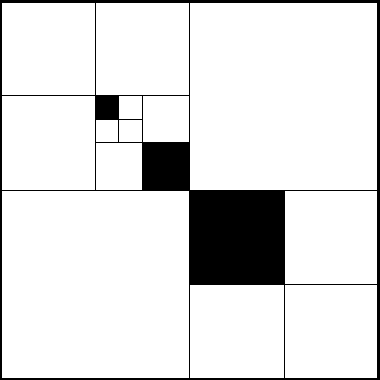
\includegraphics{figures/tikz/Hierarchical.pdf}
        \captionof{figure}{Hierarchical算法示意图,白块表示稀疏部分}
        \label{fig:Hierarchical}
    \end{center}
\end{theorem}

\begin{theorem}
    {矩阵乘法的Strassen算法}{}
    对矩阵乘法$C=AB$分块得:
    \[
        \begin{bmatrix}
            C_{11}&C_{12}\\
            C_{21}&C_{22}
        \end{bmatrix}=\begin{bmatrix}
            A_{11}&A_{12}\\
            A_{21}&A_{22}
        \end{bmatrix}\begin{bmatrix}
            B_{11}&B_{12}\\
            B_{21}&B_{22}
        \end{bmatrix},
    \]
    定义 
    \begin{subequations}
        \begin{align}
            M_1&=(A_{11}+A_{22})(B_{11}+B_{22}),\\
            M_2&=(A_{21}+A_{22})B_{11},\\
            M_3&=A_{11}(B_{12}-B_{22}),\\
            M_4&=A_{22}(B_{21}-B_{11}),\\
            M_5&=(A_{11}+A_{12})B_{22},\\
            M_6&=(A_{21}-A_{11})(B_{11}+B_{12}),\\
            M_7&=(A_{12}-A_{22})(B_{21}+B_{22}),
        \end{align}
    \end{subequations}
    则
    \begin{subequations}
        \begin{align}
            C_{11}&=M_1+M_4-M_5+M_7,\\
            C_{12}&=M_3+M_5,\\
            C_{21}&=M_2+M_4,\\
            C_{22}&=M_1-M_2+M_3+M_6.
        \end{align}
    \end{subequations}
    Strassen算法将分块矩阵的乘法从直接法的8次降低到了7次,由此分而治之,矩阵乘法的时间复杂度便从$\bigo(n^3)$降低到了$\bigo(n^{\log_27})=\bigo(n^{2.807})$。
\end{theorem}

\begin{definition}
    {离散Fourier变换}{discrete Fourier transform}
    式\eqref{eqn:Fourier betaj}中定义了一个线性变换,称为离散Fourier变换(discrete Fourier transform, DFT)
    \[
        X_n=\sum_{m=0}^{N-1}x_m\omega^{mn},
    \]
    其中$\omega:=\e{-\i2\pi/N}$是$N$次单位根,对应的变换矩阵为
    \begin{eqnarray}
        F=\begin{bmatrix}
            1&1&1&\cdots&1\\
            1&\omega&\omega^2&\cdots&\omega^{N-1}\\
            1&\omega^2&(\omega^2)^2&\cdots&(\omega^2)^{N-1}\\
            \vdots&\vdots&\vdots&\ddots&\vdots&\\
            1&\omega^{N-1}&(\omega^{N-1})^2&\cdots&(\omega^{N-1})^{N-1}
        \end{bmatrix}
    \end{eqnarray}
    事实上$F$上只有$n$个不同的元素。其逆变换为
    \begin{equation}
        F\iv=\frac1N\bar F.
    \end{equation}
\end{definition}

\begin{theorem}
    {Cooley-Tukey快速Fourier变换}{Cooley-Tukey fast Fourier transform}
    以基2 (radix-2)的情形为例,即$N=2^M$。
    将$X_n$的求和分成偶数项$E_n$和奇数项$O_n$
    \begin{align*}
        X_n&=\sum_{k=0}^{N/2-1}x_{2k}\omega^{2kn}+\sum_{k=0}^{N/2-1}x_{2k+1}\omega^{(2k+1)n}\\
        &=\sum_{k=0}^{N/2-1}x_{2k}\omega^{2kn}+\omega^n\sum_{k=0}^{N/2-1}x_{2k+1}\omega^{2kn}=:E_n+\omega^nO_n,
    \end{align*}
    由于$\omega^N=1$,注意到
    \begin{align*}
        X_{n+N/2}&=\sum_{k=0}^{N/2-1}x_{2k}\omega^{2k(n+N/2)}+\sum_{k=0}^{N/2-1}x_{2k+1}\omega^{(2k+1)(n+N/2)}\\
        &=\sum_{k=0}^{N/2-1}x_{2k}\omega^{2kn}-\omega^n\sum_{k=0}^{N/2-1}x_{2k+1}\omega^{2k}=E_n-\omega^nO_n,
    \end{align*}
    由此便将$N$个$X_n$求和($N^2$)转化成了$N/2$个$E_n,O_n$求和($N^2/2$)。
    采用分而治之的算法思想,可以将DFT的时间复杂度从矩阵向量乘法的$\bigo(N^2)$优化到$\bigo(N\log N)$,这称为快速Fourier变换(fast Fourier transform, FFT)。
    \begin{center}
        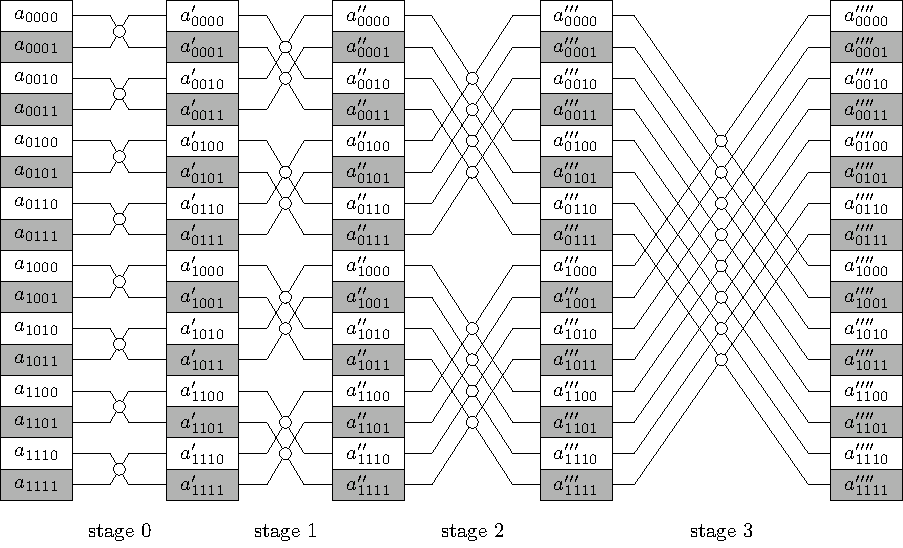
\includegraphics[width=0.8\linewidth]{figures/tikz/FFT.pdf}
        \captionof{figure}{FFT算法示意图($N=2^3=8$),\href{https://tikz.net/fast-fourier-transform/}{作者:Alexandros Tsagkaropoulos}}
        \label{fig:FFT}
    \end{center}
    \tcblower
    对于非基2的情形,$\omega^k$的周期不是基2的,做处理:
    \[
        X_n=\sum_{m=0}^{N-1}x_m\omega^{-mn}=\sum_{m=0}^Nx_m\omega^{[(m-n)^2-m^2-n^2]/2}.
    \]
    定义$\nu_k:=\omega^{k^2/2}$,记$Y_n:=\nu_nX_n,\;z_m:=\nu_m\iv x_m$,则有卷积形式:
    \[
        Y_n=\sum_{m=0}^{N-1}z_m\nu_{m-n}.
    \]
    可以用0将$z_m,\nu_m$延拓,使其周期是一个比$N$大的基2数$N'$。
    再在两端做DFT:
    \begin{align*}
        \sum_{n=0}^{N'-1}Y_n\omega_{N'}^{nk}&=\sum_{n=0}^{N'-1}\sum_{m=0}^{N'-1}z_m\nu_{m-n}\omega_{N'}^{nk}\\
        &=\sum_{m=0}^{N'-1}z_m\omega_{N'}^{mk}\sum_{n=0}^{N'-1}\nu_{m-n}\omega_{N'}^{(n-m)k}=\sum_{m=0}^{N'-1}z_m\omega_{N'}^{mk}\sum_{m=0}^{N'-1}\nu_m\omega_{N'}^{mk}
    \end{align*}
    因此通过对$z_m,\nu_m$做两次DFT、一次向量分量积、一次逆DFT便可得到$Y_n$。
\end{theorem}

\begin{theorem}
    {周期Toeplitz变换}{periodic Toeplitz transform}
    $n$阶矩阵$A$若满足$a_{ij}=c_{i-j}$且序列$c_k$周期为$n$,则$A$称为周期Toeplitz矩阵,且
    \begin{equation}
        A=F\iv\Lambda F,
    \end{equation}
    其中$\Lambda=\diag(\lambda_0,\ldots,\lambda_{n-1})$且
    \begin{equation}
        \lambda_i=\sum_{j=0}^{n-1}c_j\omega^{-ij}.
    \end{equation}
\end{theorem}

\begin{remark}
    $n$阶矩阵$A$若满足$a_{ij}=c_{i-j}$,则该矩阵可以扩展成$2n$阶的周期Toeplitz矩阵。
    \[
        \begin{bmatrix}
            A&*\\ *&*
        \end{bmatrix}
    \]
\end{remark}

\section{Gauss消元法}
\label{sec:Gauss elimination}

% \paragraph{基本思路}

% 将$Ax=b$的求解问题转化为一个与之等价的容易求解的问题$\tilde A\tilde x=\tilde b$。

\subsection{Gauss消元法}

如何求解$n$元线性方程组?
Cramer法则?时间复杂度$\bigo(n\cdot(n+1)!)$这是不可接受的。

\begin{theorem}
    {Gauss消元法}{Gauss elimination}
    线性方程组形如
    \begin{equation*}
        \lhkh{\begin{aligned}
            a_{11}^{(1)}x_1+a_{12}^{(1)}x_2+\cdots+a_{1n}^{(1)}x_n&=b_1^{(1)}\\
            a_{21}^{(1)}x_1+a_{22}^{(1)}x_2+\cdots+a_{2n}^{(1)}x_n&=b_2^{(1)}\\
            &\vdots\\
            a_{n1}^{(1)}x_1+a_{n2}^{(1)}x_2+\cdots+a_{nn}^{(1)}x_n&=b_n^{(1)}
        \end{aligned}}
    \end{equation*}
    如果$a_{11}^{(1)}\neq 0$,可将第一行的$-a_{i1}^{(1)}/a_{11}^{(1)}$倍加到第$i$行($i=2,3,\ldots,n$),得到一个等价方程组
    \begin{equation*}
        \lhkh{\begin{aligned}
            a_{11}^{(1)}x_1+a_{12}^{(1)}x_2+\cdots+a_{1n}^{(1)}x_n&=b_1^{(1)}\\
            a_{22}^{(2)}x_2+\cdots+a_{2n}^{(2)}x_n&=b_2^{(2)}\\
            &\vdots\\
            a_{n2}^{(2)}x_2+\cdots+a_{nn}^{(2)}x_n&=b_n^{(2)}
        \end{aligned}}
    \end{equation*}
    如果$a_{22}^{(2)}\neq 0$,便可以此类推……最终得到一个等价的上三角线性方程组:
    \begin{equation*}
        \lhkh{\begin{aligned}
            a_{11}^{(1)}x_1+a_{12}^{(1)}x_2+\cdots+a_{1n}^{(1)}x_n&=b_1^{(1)}\\
            a_{22}^{(2)}x_2+\cdots+a_{2n}^{(2)}x_n&=b_2^{(2)}\\
            &\vdots\\
            a_{nn}^{(n)}x_n&=b_n^{(n)}
        \end{aligned}}
    \end{equation*}
    便不难从下至上地解得:$x_n=b_n^{(n)}/a_{nn}^{(n)}$,
    \begin{equation}
        x_i=\frac{1}{a_{ii}^{(i)}}\biggkh{b_{i}^{(i)}-\sum_{j=i+1}^na_{ij}^{(i)}x_j},\quad i=n-1,\ldots,2,1.
    \end{equation}
    Gauss消元法的复杂度为$\bigo(n^3)$。
\end{theorem}

\begin{remark}
    从上面的算法过程中可见,
    一旦第$k$步$a_{kk}^{(k)}=0$,(顺序) Gauss消元法就不能继续进行下去。
    但是当第$k+1,\ldots,n$行中存在$a_{ik}^{k}\neq 0$,就可以交换$k,i$行,从而使算法继续。

    此外,即使$a_{kk}^{(k)}\neq 0$但$\abs{a_{kk}^{(k)}}\ll 1$,也会出现大数除小数导致精度下降的问题。
\end{remark}

\begin{theorem}
    {列主元方法}{pivoting technique}
    在第$k$步消去之前,找到绝对值最大的主元(pivot):
    \begin{equation}
        i_k=\mathop{\arg\max}\limits_{k\leq i\leq n}\abs{a_{ik}^{(k)}},
    \end{equation}
    然后交换第$k,i_k$行。
\end{theorem}

\subsection{LU分解}

下面我们从矩阵角度考察Gauss消元法。

\begin{definition}
    {初等矩阵}{elementary matrix}
    给定(实)向量$u,v$和标量$\sigma$,形如
    \begin{equation}
        E=I-\sigma uv\tp
    \end{equation}
    的称为(实)初等矩阵(elementary matrix)。
\end{definition}

\begin{corollary}
    初等矩阵的逆也是同类型的初等矩阵:
    \begin{equation}
        (I-\sigma uv\tp)\iv=I-\frac{\sigma}{\sigma v\tp u-1}uv\tp.
    \end{equation}
\end{corollary}

\begin{example}
    {}{}
    \begin{itemize}
        \item 初等排列矩阵:
        \[
            P_{ij}=I-(e_i-e_j)(e_i-e_j)\tp=I-e_{ii}-e_{jj}+e_{ij}+e_{ji}.
        \]
        左乘初等排列矩阵即互换第$i,j$行,右乘即互换第$i,j$列;
        \item 倍加矩阵:
        \[
            I+\alpha e_ie_j\tp=I+\alpha e_{ij},
        \]
        左乘即将第$i$行的$\alpha$倍加到第$j$行上。
    \end{itemize}
\end{example}

\begin{definition}
    {初等单位下三角矩阵}{elementary lower-triangle matrix}
    形如
    \begin{equation}
        L_i=I+\ell_ie_i\tp=\begin{bmatrix}
            1\\ &\ddots\\ &&1\\ &&\ell_{i+1,i}&1\\ &&\vdots&&\ddots\\ &&\ell_{ni}&&&1
        \end{bmatrix}
    \end{equation}
    称为第$i$列的初等单位下三角矩阵。其中向量$\ell_i$的前$i$个分量为0。
\end{definition}

\begin{corollary}
    初等单位下三角矩阵的逆也是初等单位下三角矩阵
    \begin{equation}
        (I+\ell_ie_i\tp)\iv=I-\ell_ie_i\tp.
    \end{equation}
\end{corollary}

\begin{corollary}
    对角元均为1的下三角矩阵称为单位下三角矩阵,可以写成
    \[
        L=L_1L_2\cdots L_{n-1}=\begin{bmatrix}
            1\\\ell_{21}&1\\ \vdots&\vdots&\ddots\\
            \ell_{n1}&\ell_{n2}&\cdots&1
        \end{bmatrix}.
    \]
\end{corollary}

\begin{theorem}
    {矩阵的LU分解}{LU decomposition exists}
    根据Gauss消元法的过程,记
    \[
        A^{(k)}:=\begin{bmatrix}
            a_{11}^{(1)}&\cdots&a_{1k}^{(1)}&\cdots&a_{1n}^{(1)}\\
            &\ddots&\vdots&\ddots&\vdots\\
            &&a_{kk}^{(k)}&\cdots&a_{kn}^{(k)}\\
            &&\vdots&\ddots&\vdots\\
            &&a_{nk}^{(k)}&\cdots&a_{nn}^{(k)}
        \end{bmatrix},\quad
        b^{(k)}:=\begin{bmatrix}
            b_1^{(1)}\\\vdots\\b_k^{(k)}\\\vdots\\b_n^{(k)}
        \end{bmatrix},\quad\ell_k:=-\frac1{a_{kk}^{(k)}}\begin{bmatrix}
            0\\\vdots\\0\\a_{k+1,k}^{(k)}\\\vdots\\a_{nk}^{(k)}
        \end{bmatrix}.
    \]
    相应的初等单位下三角矩阵为$L_k=I+\ell_ke_k\tp$。
    增广矩阵有递推关系:
    \begin{equation}
        [A^{(k+1)}\enspace b^{(k+1)}]=L_k[A^{(k)}\enspace b^{(k)}],
    \end{equation}
    即
    \[
        A^{(n)}=L_{n-1}\cdots L_1A^{(1)},\iff A^{(1)}=L_1\iv\cdots L_{n-1}\iv A^{(n)},
    \]
    则$L=L_1\iv\cdots L_{n-1}\iv$为单位下三角矩阵,$U=A^{(n)}$为上三角矩阵,这样就将$A^{(1)}$分解成了下上三角矩阵的乘积。    
\end{theorem}

\begin{remark}
    根据Gauss消元法的过程可见,LU分解的前提是$a_{11}^{(1)},\ldots,a_{nn}^{(n)}$均不为0。
\end{remark}

\begin{theorem}
    {三角分解定理}{LU decomposition}
    给定矩阵$A$,若其顺序主子式
    \begin{equation}
        \Delta_i:=\begin{vmatrix}
            a_{11}&\cdots&a_{1i}\\
            \vdots&\ddots&\vdots\\
            a_{i1}&\cdots&a_{ii}
        \end{vmatrix},\quad i=1,\ldots,n
    \end{equation}
    均不为0,则存在唯一的单位下三角矩阵$L$和上三角矩阵$U$使得$A=LU$。
\end{theorem}
\begin{proof}
    通过数学归纳法,可证明:$a_{11}^{(1)},\ldots,a_{ii}^{(i)}\neq 0\iff\Delta_1,\ldots,\Delta_i\neq 0$,此时
    \begin{equation}
        \Delta_i=a_{11}^{(1)}\cdots a_{ii}^{(i)},
    \end{equation}
    若存在$L_1,U_1$和$L_2,U_2$使得
    \[
        A=L_1U_1=L_2U_2,
    \]
    两边左乘$L_1\iv$,右乘$U_2\iv$得到:
    \[
        U_1U_2\iv=L_1\iv L_2,
    \]
    此式左边为上三角矩阵,右边为单位下三角矩阵,故只能是单位矩阵$I$,即$U_1=U_2,L_1=L_2$。
\end{proof}

\begin{example}
    {LU分解的例子}{}
    \[
        \begin{bmatrix}
            2&1&1&0\\4&3&3&1\\8&7&9&5\\6&7&9&8
        \end{bmatrix}=\begin{bmatrix}
            1\\2&1\\4&3&1\\3&4&1&1
        \end{bmatrix}\begin{bmatrix}
            2&1&1&0\\ &1&1&1\\ &&2&2\\ &&&2
        \end{bmatrix}.
    \]
\end{example}

\begin{remark}
    $L$有$n(n-1)/2$个变量,$U$有$n(n+1)/2$个变量,可以直接由$A$确定$L,U$。
\end{remark}

\begin{theorem}
    {直接LU分解法(Doolittle分解法)}{Doolittle decomposition}
    写成分块矩阵的形式:
    \[
        L^{(k)}=\begin{bmatrix}
            1\\\ell_{n-k+1}&L^{(k-1)}
        \end{bmatrix},\quad
        U^{(k)}=\begin{bmatrix}
            u_{u-k+1,u-k+1}&u_{u-k+1}\tp\\ &U^{(k-1)}
        \end{bmatrix},
    \]
    则
    \[
        A^{(k)}=L^{(k)}U^{(k)}=\begin{bmatrix}
            u_{u-k+1,u-k+1}&u_{u-k+1}\tp\\
            u_{u-k+1,u-k+1}\ell_{n-k+1}&A^{(k-1)}+\ell_{n-k+1}u_{u-k+1}\tp
        \end{bmatrix}.
    \]
    由此可确定$u,\ell$,同时$A^{(k)}$的阶数减1.
\end{theorem}
    
\begin{remark}
    三角分解\thmref{thm:LU decomposition} 给出了LU分解的条件。
    而对于一般的可逆矩阵,也可以通过换行实现LU分解。
\end{remark}

\begin{theorem}
    {一般三角分解定理}{LUP decomposition}
    若$A$可逆,则存在排列矩阵$P$、单位下三角矩阵$L$和上三角矩阵$U$使得
    \begin{equation}
        PA=LU.
    \end{equation}
\end{theorem}

\begin{proof}
    考虑列主元方法的Gauss消元法,第$k$步交换$k,i_k$行,则
    \[
        A^{(k+1)}=L_kI_{ki_k}A^{(k)},
    \]
    即
    \[
        A^{(n)}=L_{n-1}I_{n-1,i_{n-1}}\cdots L_1I_{1i_1}A^{(1)},
        \iff
        A^{(1)}=I_{1i_1}L_1\iv\cdots I_{n-1,i_{n-1}}L_{n-1}\iv A^{(n)},
    \]
    定义
    \[
        P_k=I_{n-1,i_{n-1}}\cdots I_{ki_k},
    \]
    则$P_k\tp P_{k+1}=I_{ki_k}$,进而
    \[
        P_1A^{(1)}=P_2L_1\iv P_2\tp P_3L_2\iv\cdots P_{n-1}L_{n-1}\iv A^{(n)},
    \]
    易得$P_{k+1}e_k=e_k$,故
    \[
        L_k':=P_{k+1}L_k\iv P_{k+1}\tp=P_{k+1}(I-\ell_ke_k\tp)P_{k+1}\tp=I-P_{k+1}\ell_ke_k\tp,
    \]
    仍然是第$k$列的初等单位上三角矩阵,
    令$P=P_1,\;L=L_1'\cdots L_{n-2}'L_{n-1},\;U=A^{(n)}$即得。
\end{proof}

\subsection{Cholesky分解}

下面再看对称矩阵的三角分解。

\begin{theorem}
    {Cholesky分解}{Cholesky decomposition}
    若$A$实对称正定,则存在唯一的对角元素为正的下三角矩阵$L$使得
    \begin{equation}
        A=LL\tp.
    \end{equation}
\end{theorem}

\begin{proof}
    采用加边Cholesky分解法:写成分块矩阵的形式
    \[
        L_i=\begin{bmatrix}
            L_{i-1}\\\ell_{i-1}\tp&\ell_{ii}
        \end{bmatrix},\quad A_i=\begin{bmatrix}
            A_{i-1}&a_{i-1}\\ a_{i-1}\tp&a_{ii}
        \end{bmatrix}
    \]
    满足$A_i=L_iL_i\tp$,
    可得 
    \begin{subequations}
        \begin{align}
            \ell_{i-1}&=L_{i-1}\iv a_{i-1},\\
            \ell_{ii}&=\sqrt{a_{ii}-\ell_{i-1}\tp\ell_{i-1}}.
        \end{align}
    \end{subequations}
    从$\ell_{11}=\sqrt{a_{11}}$出发便可迭代得到整个$L$。
\end{proof}

\begin{remark}
    这种算法特别适合稀疏矩阵。
\end{remark}

\subsection{Thomas方法}

考虑线性方程组
\[
    \begin{cases}
        b_1x_1+c_1x_2=d_1,\\
        a_ix_{i-1}+b_ix_i+c_ix_{i+1}=d_i,&i=2,\ldots,n-1\\
        a_nx_{n-1}+b_nx_n=d_n
    \end{cases}
\]
系数矩阵为三对角矩阵:
\[
    \begin{bmatrix}
        b_1&c_1\\a_2&b_2&\ddots\\ &\ddots&\ddots&c_{n-1}\\ &&a_n&b_b
    \end{bmatrix}.
\]
\begin{theorem}
    {Thomas方法}{Thomas technique}
    容易验证有如下三角分解形式:
    \[
        A=LU=\begin{bmatrix}
            1\\\ell_2&1\\&\ddots&\ddots\\ &&\ell_n&1
        \end{bmatrix}\begin{bmatrix}
            u_1&c_1\\ &u_2&\ddots\\ &&\ddots&c_{n-1}\\ &&&u_n
        \end{bmatrix},
    \]
    可直接乘开得到$u_1=b_1$
    \begin{equation}
        \ell_i=\frac{a_i}{u_{i-1}},\quad u_i=b_i-\ell_ic_{i-1}.
    \end{equation}
\end{theorem}


\section{稳定性分析}
\label{sec:stability analysis}

在用直接法求解$Ax=b$的过程中,由于舍入误差的存在,必然会导致结果产生误差。因而有必要对可能产生的误差作一估计。
% 通常我们假设在数值处理的过程中计算都是精确的.
\begin{example}
    {数据的微小变化导致解的巨大变化}{}
    方程组
    \[
        \begin{bmatrix}
            10&7&8&7\\
            7&5&6&5\\
            8&6&10&9\\
            7&5&9&10
        \end{bmatrix}\begin{bmatrix}
            x_1\\x_2\\x_3\\x_4
        \end{bmatrix}=\begin{bmatrix}
            32\\23\\33\\31
        \end{bmatrix}\implies\begin{bmatrix}
            x_1\\x_2\\x_3\\x_4
        \end{bmatrix}=\begin{bmatrix}
            1\\1\\1\\1
        \end{bmatrix}.
    \]
    对向量$b$数据做微小的修改
    \[
        \begin{bmatrix}
            10&7&8&7\\
            7&5&6&5\\
            8&6&10&9\\
            7&5&9&10
        \end{bmatrix}\begin{bmatrix}
            x_1'\\x_2'\\x_3'\\x_4'
        \end{bmatrix}=\begin{bmatrix}
            32.1\\22.9\\33.1\\30.9
        \end{bmatrix}\implies\begin{bmatrix}
            x_1'\\x_2'\\x_3'\\x_4'
        \end{bmatrix}=\begin{bmatrix}
            9.2\\-12.6\\4.5\\-1.1
        \end{bmatrix}.
    \]
    对系数矩阵$A$数据做微小的修改
    \[
        \begin{bmatrix}
            10&7&8.1&7.2\\
            7.08&5.04&6&5\\
            8&5.98&9.89&9\\
            6.99&4.99&9&9.98
        \end{bmatrix}\begin{bmatrix}
            x_1''\\x_2''\\x_3''\\x_4''
        \end{bmatrix}=\begin{bmatrix}
            32\\23\\33\\31
        \end{bmatrix}\implies\begin{bmatrix}
            x_1''\\x_2''\\x_3''\\x_4''
        \end{bmatrix}=\begin{bmatrix}
            -81\\137\\-34\\22
        \end{bmatrix}.
    \]
    可见数据的微小变化会导致解的巨大变化,这是因为系数矩阵的条件数$\cond(A)=32825/11$很大。
\end{example}

\begin{definition}
    {条件数}{condition number}
    给定诱导的矩阵范数$\norm\cdot$,可逆矩阵$A$的条件数(condition number)为
    \begin{equation}
        \cond(A)\equiv\norm A\nnorm{A\iv}.
    \end{equation}
\end{definition}

\begin{corollary}
    条件数的性质:
    \begin{itemize}
        \item $\cond(A)\geq 1$;
        \item $\cond(A\iv)=\cond(A)$;
        \item $\cond(cA)=\cond(A)$;
        \item 若$U$为正交矩阵,则$\cond_2(U)=1$,且
        \begin{equation}
            \cond_2(A)=\cond_2(AU)=\cond_2(UA);
        \end{equation}
        \item 若$\lambda_1,\lambda_n$是$A$模最大与最小的特征值,则
        \begin{equation}
            \cond(A)\geq\frac{\abs{\lambda_1}}{\abs{\lambda_n}},
        \end{equation}
        若$A$对称,则$\cond_2(A)=\abs{\lambda_1}/\abs{\lambda_n}$;
        \item 由范数的等价性,可知条件数的等价性:
        \begin{subequations}
            \begin{alignat}{4}
                \frac1n&\cond_2&(A)&\leq\cond_1&(A)&\leq n\cond_2&(A),\\
                \frac1n&\cond_\infty&(A)&\leq\cond_2&(A)&\leq n\cond_\infty&(A),\\
                \frac1{n^2}&\cond_1&(A)&\leq\cond_\infty&(A)&\leq n^2\cond_1&(A).
            \end{alignat}
        \end{subequations}
    \end{itemize}
\end{corollary}

\begin{theorem}
    {解的扰动定理}{}
    给定可逆矩阵$A$和微小扰动$\D A$,满足
    \[
        \frac{\norm{\D A}}{\norm A}<\frac1{\cond(A)},
    \]
    则$(A+\D A)$也可逆,考察线性方程组$Ax=b$及其扰动方程组
    \[
        (A+\D A)(x+\D x)=b+\D b,
    \]
    则有
    \begin{equation}
        \frac{\norm{\D x}}{\norm x}\leq\frac{\cond(A)}{1-\norm{A\iv}\norm{\D A}}\biggkh{\frac{\norm{\D A}}{\norm A}+\frac{\norm{\D b}}{\norm b}}.
    \end{equation}
\end{theorem}

\begin{proof}
    由扰动定理\thmref{thm:perturbation theorem II} 知$(A+\D A)$可逆且
    \begin{equation}
        \norm{(A+\D A)\iv}\leq\frac{\norm{A\iv}}{1-\norm{A\iv}\norm{\D A}}.
    \end{equation}
    由
    \begin{align*}
        \D x&=(A+\D A)\iv(b+\D b)-x\\
        &=(A+\D A)\iv(b+\D b-(A+\D A)x)\\
        &=(A+\D A)\iv(\D b-\D Ax),
    \end{align*}
    两边取范数
    \begin{align*}
        \norm{\D x}&\leq\norm{(A+\D A)\iv}(\norm{\D b}+\norm{\D A}\norm x)\\
        &\leq\frac{\norm{A\iv}}{1-\norm{A\iv}\norm{\D A}}\biggkh{\frac{\norm{\D A}}{\norm A}\norm A\norm x+\frac{\norm{\D b}}{\norm b}\norm A\norm x}.
        \qedhere
    \end{align*}
\end{proof}

\begin{remark}
    因此条件数可以看成扰动方程组相对误差的放大倍数。
\end{remark}

\begin{theorem}
    {矩阵相对奇异性的度量}{relative singularity}
    若$A$可逆,定义所有使得$(A+\D A)$不可逆的$\D A$构成集合$S$,则 
    \begin{equation}
        \min_{\D A\in S}\frac{\norm{\D A}_2}{\norm A_2}=\frac1{\cond_2(A)},
    \end{equation}
\end{theorem}

\begin{proof}
    当$\nnorm{A\iv}\norm{\D A}<1$时,$(A+\D A)$可逆,故
    \[
        \min_{\D A\in S}\norm{\D A}_2\geq\frac1{\norm{A\iv}_2}.
    \]
    由$\norm\cdot_2$的定义,$\exists x$且$\norm x_2=1$使得$\norm{A\iv x}_2=\norm{A\iv}_2$,令$y=A\iv x/\nnorm{A\iv}_2$,并取
    \[
        \D A=-\frac{xy\tp}{\norm{A\iv}_2},
    \]
    则$\norm y_2=1$且
    \[
        (A+\D A)y=\frac{x}{\norm{A\iv}_2}-\frac{xy\tp y}{\norm{A\iv}_2}=0,
    \]
    故$(A+\D A)$不可逆,又
    \[
        \norm{\D A}_2=\max_{\norm z_2=1}\norm{\D Az}_2=\frac{\norm x_2}{\norm{A\iv}_2}\max_{\norm z_2=1}\abs{y\tp z}=\frac1{\norm{A\iv}_2}.
        \qedhere
    \]
\end{proof}

\begin{remark}
    因此可逆矩阵到最接近的奇异矩阵的相对距离在2 - 范数意义下就是2 - 条件数的倒数。当条件数很大时,矩阵与奇异矩阵的相对距离很小,称为病态(ill conditioned)。
\end{remark}

\begin{theorem}
    {近似解的相对误差}{}
    若$x,x'$分别是方程组$Ax=b$的精确解和近似解,$x'$的剩余$r=b-Ax'$,则
    \begin{equation}
        \frac1{\cond(A)}\frac{\norm r}{\norm b}\leq\frac{\norm{x'-x}}{\norm x}\leq\cond(A)\frac{\norm r}{\norm b}.
    \end{equation}
\end{theorem}

\begin{proof}
    由$A(x'-x)=-r$和$\norm A\norm x\geq\norm b$可得
    \[
        \norm r\leq\norm A\norm{x'-x}=\frac{\cond(A)}{\norm{A\iv}}\norm{x'-x},
    \]
    两边除$\norm b$,由$x=A\iv b$可得 
    \[
        \frac{\norm r}{\norm b}\leq\cond(A)\frac{\norm{x'-x}}{\norm{A\iv}\norm b}\leq\cond(A)\frac{\norm{x'-x}}{\norm x};
    \]
    另一方面,由$x'-x=-A\iv r$可得
    \[
        \norm{x'-x}=\norm{A\iv r}\leq\norm{A\iv}\norm r=\cond(A)\frac{\norm r}{\norm A}.
    \]
    两边同除$\norm x$,由$Ax=b$可得 
    \[
        \frac{\norm{x'-x}}{\norm x}\leq\cond(A)\frac{\norm r}{\norm A\norm x}\leq\cond(A)\frac{\norm r}{\norm b}.
    \]
    综上,两边不等式均得证。
\end{proof}

\begin{remark}
    这说明当方程组病态时,即使剩余$\norm r$比较小,解的相对误差仍可能很大。
\end{remark}

\begin{example}
    {Hilbert矩阵}{Hilbert matrix}
    Hilbert矩阵
    \begin{equation*}
        H_n:=\begin{bmatrix}
            1&1/2&\cdots&1/(n+1)\\
            1/2&1/3&\cdots&1/(n+2)\\
            \vdots&\vdots&\ddots&\vdots\\
            1/(n+1)&1/(n+2)&\cdots&1/(2n+1)
        \end{bmatrix}
    \end{equation*}
    的条件数增长很快:
    \[
        \cond_2(H_n)=\bigo\biggkh{\frac{(1+\sqrt2)^{4n}}{\sqrt n}}.
    \]
\end{example}

\begin{theorem}
    {条件数与数值精度}{}
    用直接法解方程组$Ax=b$,$A,b$的元素有效位数为$s$而$\cond(A)$的数量级为$t$,则求得$x$分量有效位数约为$s-t$。
\end{theorem}

\paragraph{病态方程组的解法}

除采用更高精度的运算外,另一个更有效的方法是对原方程进行预处理:
\[
    Ax=b,\iff PAQ(Q\iv x)=Pb,
\]
从而降低系数矩阵的条件数:$\cond(PAQ)\ll\cond(A)$。一般$P,Q$可选择为三角矩阵或对角矩阵。

\begin{example}
    {预处理例子}{}
    方程组
    \[
        \begin{bmatrix}
            10&10^5\\1&1
        \end{bmatrix}\begin{bmatrix}
            x_1\\x_2
        \end{bmatrix}=\begin{bmatrix}
            10^5\\2
        \end{bmatrix}\implies\begin{bmatrix}
            x_1\\x_2
        \end{bmatrix}=\frac1{9999}\begin{bmatrix}
            10000\\9998
        \end{bmatrix}.
    \]
    系数矩阵的条件数$\cond_2(A)=100010$很大,左乘$D=\diag(10^{-5},1)$平衡:
    \[
        \begin{bmatrix}
            10^{-4}&1\\1&1
        \end{bmatrix}\begin{bmatrix}
            x_1\\x_2
        \end{bmatrix}=\begin{bmatrix}
            1\\2
        \end{bmatrix},
    \]
    系数矩阵的条件数$\cond_2(DA)=940/359$得到了有效降低。
\end{example}


\chapter{特征值和特征向量}
\section{特征值和特征向量}
\begin{definition}{特征值和特征向量}{eigenvalue and eigenvector}
	给定方阵$A$,若存在$x\neq 0$和$\lambda\in\FF$满足:
	\[
		Ax=\lambda x,
	\]
	则称$x$是$A$的特征向量(eigenvector),$\lambda$是对应的特征值(eigenvalue)。
	矩阵$A$所有特征值构成的集合称为$A$的谱(spectrum)。
\end{definition}

\begin{corollary}
	特征值的性质:
	\begin{compactenum}
		\item $A$的特征向量$x$也是$A^n$的特征向量,特征值是$\lambda^n;$
		\item 若$A$可逆,则$x$也是$A\iv$的特征向量,特征值是$\lambda^{-1};$
		\item 三角矩阵的特征值就是对角元;
		\item $A$可逆$\iff A$所有特征值非0。
		
		% 只需注意到$A$可逆时$Ax=0$只有零解即可。
	\end{compactenum}
\end{corollary}

\begin{theorem}{不同特征值对应特征向量线性无关}{eigenvalue}
	给定$A$的一组特征向量$x_1,\ldots,x_r$,对应特征值为$\lambda_1,\ldots,\lambda_r$。
	若$\lambda_1,\ldots,\lambda_r$两两不等,则$x_1,\ldots,x_r$线性无关。
\end{theorem}
\begin{proof}
	运用数学归纳法证明。$r=1$时,$x_1\neq 0$自然线性无关;
	
	假设$r=m-1$时,$x_1,\ldots,x_{m-1}$线性无关;当$r=m$时,考虑
	\begin{equation}
		\label{eqn:proof eigen 1}
		x_m=c_1x_1+\cdots+c_{m-1}x_{m-1},\tag{$\ast$}
	\end{equation}
	两边同时左乘$A$得
	\begin{equation}
		\label{eqn:proof eigen 2}
		\lambda_mx_m=c_1\lambda_1x_1+\cdots+c_{m-1}\lambda_{m-1}x_{m-1},\tag{$\ast\ast$}
	\end{equation}
	$\lambda_m$\eqref{eqn:proof eigen 1} $-$ \eqref{eqn:proof eigen 2}得,
	\[
		0=c_1(\lambda_m-\lambda_1)x_1+\cdots+c_{m-1}(\lambda_m-\lambda_{m-1})x_{m-1},
	\]
	由$x_1,\ldots,x_{m-1}$线性无关可得所有的$c_i=0$,故$x_1,\ldots,x_m$线性无关。

	综上,定理对所有可能的$r$均成立。
\end{proof}

\section{特征多项式}

\begin{definition}{特征子空间}{eigen-subspace}
	$A$的所有特征值为$\lambda$的特征向量张成$\RR^n$的一个线性子空间:$\N(A-\lambda I).$
\end{definition}

% \begin{corollary}
% 	如果$\lambda$是$A$的特征值,则$(A-\lambda I)$必然不可逆。
% \end{corollary}

\begin{definition}
	{特征方程和特征多项式}{eigenfunction and eigen-polynomial}
	求特征值$\lambda$需要解特征方程(eigenfunction):
	\[
		\det(\lambda I-A)=\lambda^n+a_1\lambda^{n-1}+\cdots+a_n=0,
	\]
	而$p_A(\lambda):=\det(\lambda I-A)$称为特征多项式(eigen-polynomial)。
\end{definition}

\begin{corollary}
	特别地,$p_A(0)=a_n=\det(-A)$,由Vieta定理:在考虑重根的情况下,
	\begin{equation}
		\label{eqn:det lambda}
		\det(A)=\prod_{i=1}^n\lambda_i.
	\end{equation}
	另一方面,通过对行列式进行Laplace展开,可得$a_1=-\tr(A)$,由Vieta定理:
	\begin{equation}
		\label{eqn:trace lambda}
		\tr(A)=\sum_{i=1}^n\lambda_i,
	\end{equation}
\end{corollary}

\subsectionstar{Cayley-Hamilton定理}

\begin{theorem}
	{Cayley-Hamilton定理}{Cayley-Hamilton theorem}
	给定特征多项式$p_A$的系数$1,a_1,\ldots,a_n$,可定义矩阵多项式
	\begin{equation}
		p_A^*(X)=X^n+a_1X^{n-1}+\cdots+a_{n-1}X+a_nI,
	\end{equation}
	则$p_A^*(A)=O$。
\end{theorem}

\noindent
\textit{完全错误的证明.}
将特征多项式$p_A(\lambda)=\det(\lambda I-A)$中的$\lambda$替换为$A$,自然得到$p_A(A)=\det(AI-A)=0$。

% \begin{proof}
% 	仅证明$A$的特征向量$x_1,\ldots,x_n$构成$\FF^n$的一组基的情形(即$A$可对角化),
% 	\begin{align*}
% 		p_A(A)x_i&=A^nx_i+c_{n-1}A^{n-1}x_i+\cdots+c_0x_i\\
% 		&=\lambda_i^2x_i+c_{n-1}\lambda_i^{n-1}x_i+\cdots+c_0x_i=p_A(\lambda)x_i=0,
% 	\end{align*}
% 	故$\forall x\in\FF^n$,都有$p_A(A)x=0$,取$x=e_1,\ldots,e_n$可得$p_A(A)=O$。
% \end{proof}

% \begin{remark}
% 	特征多项式$p_A:\FF\to\FF$与矩阵多项式$p_A^*$是完全不同的两个映射。
% \end{remark}

\begin{proof}
	考察伴随矩阵$\adj(\lambda I-A)$,可以写成如下形式:
	\[
		\adj(\lambda I-A)=B_1\lambda^{n-1}+\cdots+B_{n-1}\lambda+B_n,
	\]
	其中$B_1,\ldots,B_n$完全由$A$决定。
	由伴随矩阵的性质:
	\[
		(\lambda I-A)\adj(\lambda I-A)=\det(\lambda I-A)I=p_A(\lambda)I,
	\]
	两边展开可得
	\[
		B_1\lambda^n+(B_2-AB_1)\lambda^{n-1}+\cdots+(B_n-AB_{n-1})\lambda-AB_n=I\lambda^n+a_1I\lambda^{n-1}+\cdots+a_{n-1}\lambda+a_nI,
	\]
	作为系数的矩阵均由$A$确定,与$\lambda$无关。由于上式$\forall\lambda$均成立,故对应系数相同:
	\[
		B_1=I,\quad
		B_{i+1}-AB_i=a_iI,\quad
		-AB_n=a_nI.
	\]
	因而$p_A^*(A)$可以化为裂项和(telescoping sum)
	\[
		p_A^*(A)=A^nB_1+A^{n-1}(B_2-AB_1)+\cdots+A(B_n-AB_{n-1})-AB_n=O.
		\qedhere
	\]
\end{proof}

\begin{theorem}
	{Faddeev-LeVerrier算法}{Faddeev-LeVerrier algorithm}
	特征多项式$p_A(\lambda)$的第$k$个系数$a_k$可以递归地求出:
	\begin{equation}
		a_k=-\frac1k\bigfkh{\tr(A^k)+a_1\tr(A^{k-1})+\cdots+a_{k-1}\tr(A)}.
		% a_m=-\frac1m\sum_{k=1}^ma_{m-k}\tr(A^k).
	\end{equation}
\end{theorem}

\begin{proof}
	沿用\thmref{thm:Cayley-Hamilton theorem} 证明中的定义,
	% 并额外定义$B_0=O,\enspace c_0=1$。
	% 两边取迹得
	% \[
	% 	(n-i)a_i=\tr(AB_i)+na_i
	% \]
	由Jacobi公式\eqref{eqn:Jacobi det'},有 
	\[
		p_A'(\lambda)=\tr(\adj(\lambda I-A)I)=\tr(B_1\lambda^{n-1}+\cdots+B_n)
	\]
	展开
	\[
		n\lambda^{n-1}+(n-1)a_1\lambda^{n-2}+\cdots+a_{n-1}=\tr(B_1)\lambda^{n-1}+\tr(B_2)\lambda^{n-2}+\cdots+\tr(B_n).
	\]
	由于上式$\forall\lambda$均成立,故对应系数相同:
	\[
		(n-k)a_k=\tr(B_{k+1}),
	\]
	又$B_k$满足递推关系$B_{k+1}=AB_k+a_kI$,两边取迹可得
	\[
		(n-k)a_k=\tr(AB_k)+na_k,\implies a_k=-\frac1k\tr(AB_k),
	\]
	再展开$B_k$即证:
	\[
		B_k=AB_{k-1}+a_{k-1}I=\cdots=A^{k-1}+a_1A^{k-2}+\cdots+a_{k-1}I.
		\qedhere
	\]
\end{proof}

\begin{corollary}
	取$\lambda=0$可得伴随矩阵:
	\begin{equation}
		\adj(-A)=B_n=A^{n-1}+a_1A^{n-2}+\cdots+a_{n-1}I.
	\end{equation}
	易证这满足$\adj(-A)(-A)=(-A)\adj(-A)=\det(-A)I=c_0I$。
\end{corollary}

\begin{example}
	{特征多项式的前几项}{}
	\begin{subequations}
		\begin{align}
			a_2&=\frac12\bigkh{\tr(A)^2-\tr(A^2)},\\
			a_3&=\frac16\bigkh{\tr(A)^3-3\tr(A)\tr(A^2)+2\tr(A^3)},
		\end{align}
	\end{subequations}
	更一般地,$a_k$的显性表达式由一个$k$阶行列式给出:
	\begin{equation}
		a_k=\frac{(-)^k}{k!}\begin{vmatrix}
			\tr(A)&k-1\\
			\tr(A^2)&\tr(A)&k-2\\
			\vdots&\vdots&\ddots&\ddots\\
			\vdots&\vdots&\vdots&\ddots&1\\
			\tr(A^k)&\tr(A^{k-1})&\tr(A^{k-2})&\cdots&\tr(A)
		\end{vmatrix}.
	\end{equation}
\end{example}

\section{矩阵对角化}

由于对角矩阵有很多简单的性质,考虑相似变换$\Lambda=X\iv AX$,其中$\Lambda$为对角矩阵。

\begin{theorem}{相似变换与特征多项式}{}
	$A$的相似变换$B\iv AB$和$A$有相同的特征多项式。
\end{theorem}
\begin{proof} 
	对下式两边取行列式即证。
	\[
		\lambda I-B\iv AB=\lambda B\iv IB-B\iv AB=B\iv(\lambda I-A)B.
		\qedhere
	\]
\end{proof}

\begin{theorem}{可对角化判定}{}
	$n$阶矩阵$A$可对角化$\iff A$有$n$个线性无关的特征向量$x_1,\ldots,x_n$。
	\tcblower
	此时$A=X\Lambda X\iv$,$X$由特征向量给出,对角矩阵$\Lambda$由对应特征值$\lambda_1,\ldots,\lambda_n$ (可能相同)给出:
	\begin{align}
		X=(x_1,\ldots,x_n),\quad\Lambda=\diag(\lambda_1,\ldots,\lambda_n).
	\end{align}
\end{theorem}
\begin{proof}
	假设$A$有$n$个线性无关的特征向量$x_1,\ldots,x_n$,
	\[
		AX=(Ax_1,\ldots,Ax_n)=(\lambda_1x_1,\ldots,\lambda_nx_n)=X\Lambda,
	\]
	故$A$可对角化;反过来说,若$A$可对角化为$X\Lambda X\iv$,则$AX=X\Lambda$,即
	\[
		(Ax_1,\ldots,Ax_n)=(\lambda_1x_1,\ldots,\lambda_nx_n),
	\]
	故$x_1,\ldots,x_n$是$A$的特征向量,又$X$可逆,故$x_1,\ldots,x_n$线性无关。
\end{proof}
\begin{corollary}
	有$n$个互不相同特征值的$n$阶矩阵$A$可对角化。
\end{corollary}

\paragraph{特征值的重数}

当特征值重复时,引入两个概念
\begin{definition}{几何重数和代数重数}{}
	几何重数(geometric multiplicity, GM):特征值$\lambda$对应的最大线性无关的特征向量的个数,即$\dim\bigkh{\N(\lambda I-A)}$。

	代数重数(algebraic multiplicity, AM):特征值$\lambda$作为特征方程$\det(\lambda I-A)=0$的根的重复次数。
\end{definition}
特征方程可以写成
\[
	\prod_{i=1}^r(\lambda-\lambda_i)^{m_i}=0,
\]
其中$\lambda_i$是互不相同的根,$m_i$是$\lambda_i$的代数重数。
\begin{theorem}{}{GM <= AM}
	GM $\leqslant$ AM.
\end{theorem}
\begin{proof}
	考虑$n$阶矩阵$A$,假设特征值$\lambda_1$的GM $=\dim(\lambda_1I-A)=m$,
	
	取$\{x_1,\ldots,x_m\}$为$\C(\lambda_1I-A)$的一组正交归一基。
	
	取$\{b_1,\ldots,b_{n-m}\}$为$\N(\lambda_1I-A)^\perp$的一组正交归一基。
	
	设$n\times n$矩阵 
	\[
		P=(x_1,\ldots,x_m,b_1,\ldots,b_{n-m})=(X,B),
	\]
	$P$是可逆的且$P\iv=P\tp$,且$X\tp B=0$,则 
	\[
		P\iv AP=\begin{bmatrix}
			\lambda_1I_m&X\tp AB\\0&B\tp AB
		\end{bmatrix},
	\]
	分块三角矩阵
	\[
		\det(\lambda I-P\iv AP)=(\lambda-\lambda_1)^m\det(\lambda I-B\tp AB),
	\]
	$A$和$P\iv AP$有相同的特征方程,故$\lambda_1$必然是$A$的特征方程的根,且其AM $\geqslant$ GM。
\end{proof}
\begin{corollary}
	$n$阶矩阵$A$的全部特征值为$\{\lambda_1,\ldots,\lambda_r\}$,$A$可对角化当且仅当
	\[
		\sum_{i=1}^r\dim(\lambda_iI-A)=n,
	\]
	即所有特征值的AM = GM。
\end{corollary}
\begin{theorem}{同时对角化}{}
	若$A,B$可对角化,则他们可以同时对角化当且仅当$AB=BA$。
\end{theorem}
\begin{proof}
	若$A,B$可以同时对角化,故
	\[
		A=X\Lambda_AX\iv,\quad B=X\Lambda_BX\iv,
	\]
	故
	\[
		AB-BA=X(\Lambda_A\Lambda_B-\Lambda_B\Lambda_A)X\iv=0;
	\]
	
	若$AB=BA$,下证$A,B$可同时对角化。
	
	设$A$的特征值为$\{\lambda_1,\ldots,\lambda_s\}$,$\lambda_i$对应特征子空间为$V_i$,几何重数$m_i=\dim(V_i)$,%为方便,
	记$n_i:=m_1+\cdots+m_{i-1}$,
	取$\{v_{n_i+1},\ldots,v_{n_i+m_i}\}$表示$V_i$的一组基,记$X=(v_1,\ldots,v_n)$,则$X$可对角化$A$
	\[
		X\iv AX=\begin{bmatrix}
			\lambda_1I_{m_1}\\ &\ddots\\ &&\lambda_sI_{m_s}
		\end{bmatrix},
	\]
	$\forall x\in V_i$,
	\[
		(AB-BA)x=(A-\lambda_iI)Bx=0,
	\]
	故$Bx\in V_i$,从而$X\iv BX$和$X\iv AX$一样是分块对角的:
	\[
		X\iv BX=\begin{bmatrix}
			B_1\\ &\ddots\\ &&B_s
		\end{bmatrix},
	\]
	其中$B_i$是$m_i\times m_i$的。给定$B$的特征值$\xi_j$,其必是$B_1,\ldots,B_s$其中至少一个的特征值,不妨考虑$\xi_j$是$B_i$的特征值\footnote{无需考虑$\N(B_i)$},若$\xi_j$的AM $>B_i$的GM,则$\xi_j$的AM $>B$的GM,$B$便不能被对角化,与前提矛盾!故$B_i$均可被特定的$Y_i$对角化,即$Y_i\iv B_iY_i=\Lambda_i$,构造
	\[
		Y=\begin{bmatrix}
			Y_1\\ &\ddots\\ &&Y_s
		\end{bmatrix}
	\]
	则$Y\iv X\iv BXY$是对角化的,同时$Y\iv X\iv AXY$也是对角化的,取$Z=XY$,便可同时对角化$A,B$。
\end{proof}
\sectionstar{Jordan标准型}
不是所有方阵都可以对角化,如果$n$阶矩阵$A$有$r<n$个线性独立的特征向量,怎么把$A$变成最接近对角矩阵的形式?

\begin{theorem}{Jordan标准型}{Jordan normal form}
	$n$阶矩阵$A$有$r$个特征值,则存在$B$,使得
	\[
		B^{-1}AB=\begin{bmatrix}
			J_1             \\
			 & \ddots       \\
			 &        & J_r
		\end{bmatrix},\quad
		J_i=\begin{bmatrix}
			\lambda_i & 1                              \\
			          & \lambda_i & \ddots             \\
			          &           & \ddots & 1         \\
			          &           &        & \lambda_i
		\end{bmatrix}
	\]
	其中$J_i$称为Jordan块,$\lambda_i$是$A$的第$i$个特征值。
\end{theorem}
其证明是线性代数的核心。其中一些概念需要等到\chapref{chap:linear mapping}线性映射才会提及。先给出几个概念证明引理。
\begin{definition}{广义特征向量}{general eigenvector}
	线性映射$T:V\to V$的广义特征向量(general eigenvector) $v\in V$且$v\neq 0$,使得$(T-\lambda I)^kv=0$对某个正整数$k$成立。这里$I:V\to V$是恒等映射。

	使得$(T-\lambda I)^dv=0$成立的最小正整数$d$称为$v$的幂指数(exponent)。
\end{definition}
\begin{theorem}{}{}
	给定正整数$k$,广义特征方程$(T-\lambda I)^kv=0$有解当且仅当$\lambda$是$T$的特征值。
\end{theorem}
\begin{proof}
	若$\lambda$是$T$的特征值,则$(T-\lambda I)v=0$,左乘$(T-\lambda I)^{k-1}$即可。
	
	若$(T-\lambda I)^kv=0$有解,则$w=(T-\lambda I)^{k-1}v$满足$(T-\lambda I)w=0$,$\lambda$是$T$的特征值。
\end{proof}
\begin{theorem}{}{}
	令$u_i:=(T-\lambda I)^iv$,则$B=\{u_0,\ldots,u_{d-1}\}$是一组线性无关的向量。
\end{theorem}
\begin{proof}
	设
	\[
		\sum_{i=0}^{d-1}a_iu_i=\sum_{i=0}^{d-1}a_i(T-\lambda I)^iv=0,
	\]
	左乘$(T-\lambda I)^{d-1}$,左边只剩$a_0(T-\lambda I)^{d-1}v$,故$a_0=0$;
	
	递推地左乘$(T-\lambda I)^{d-2},(T-\lambda I)^{d-3},\ldots$可得到所有系数为0,从而$u_0,\ldots,u_{d-1}$线性无关。
\end{proof}
\begin{theorem}{}{}
	\[
		Tu_j=\begin{cases}
			\lambda u_j+u_{j+1},&1\leqslant j<d-1\\
			\lambda u_j,&j=d-1\\
			0,&j>d-1
		\end{cases}
	\]
\end{theorem}
\begin{proof}
	$1\leqslant j<d-1$时,$(T-\lambda I)u_j=u_{j+1}$,即$Tu_j=\lambda u_j+u_{j+1}$。
	
	$j=d-1$时,$(T-\lambda I)u_j=0$,即$Tu_j=\lambda u_j$;
	
	$j>d-1$时,$u_j=0$。
\end{proof}
\begin{theorem}{}{}
	$X=\lspan(B)$是$T$的不变子空间,即$T(X)\subset X$
\end{theorem}
\begin{proof}
	由上式,$\forall u=a_0u_0+\cdots+a_{d-1}u_{d-1}\in X$
	\[
		Tu=\sum_{i=0}^{d-2}a_i(\lambda u_i+u_{i+1})+a_{d-1}\lambda u_{d-1}\in X.
	\]
	因为$X$是$T$的不变子空间,我们可以把$T$看成是$X\to X$的线性映射。
	取$B$作为$X$的一组基,则$T$在$B$下的表示矩阵为
	\[
		T=\begin{bmatrix}
			\lambda\\ 1&\lambda\\ &\ddots&\ddots\\ &&1&\lambda
		\end{bmatrix}
	\]
	这与Jordan块在\thmref{thm:Jordan normal form} 中的定义仅仅是转置的差别。
\end{proof}

接下来我们将证明$V$中存在一组基,$T$在这组基上的表示矩阵是分块对角的,而且每一块都是Jordan块的形式。
\begin{theorem}{}{}
	若$v_1,\ldots,v_r$是$T$的广义特征向量,且相应的幂指数是$d_i$,设 
	\[
		u_{ij}:=(T-\lambda_iI)^jv_i,\quad V_i:=\lspan(u_{i0},\ldots,u_{id-1}).
	\]
	之前证明了$V_i$是$T$的不变子空间,且$T$在$V_i$上的表示矩阵是Jordan块。故
	$T$在$V_1\oplus\cdots\oplus V_r$上的表示矩阵是分块对角的,且每一块都是Jordan块的形式。
\end{theorem}
%平凡的。
所以我们只要证明存在这样一组广义特征向量$v_1,\ldots,v_r$使得$V=V_1\oplus\cdots\oplus V_r$就可以证明Jordan标准型的定理。

假设$\lambda$是$T$的某个特征值。如果$T-\lambda I$可以写成Jordan块的形式,则$T$也可以写成Jordan块的形式。所以以下我们用$T-\lambda I$代替$T$,或者说,考虑有一个特征值是0的线性映射$T$。
\begin{theorem}{}{}
	设$K_i=\ker(T^i),\,U_i=\Im(T^i)$,则
	\[
		K_1\subset K_2\subset\cdots,\quad U_1\supset U_2\supset\cdots
	\]
\end{theorem}
\begin{proof}
	待补
\end{proof} 

\section{对称矩阵}

\begin{definition}
	{对称矩阵}{symmetric matrix}
	若$S\tp=S$,则称$S$是对称矩阵(symmetric matrix);
	
	若$A\tp=-A$,则称$A$是反对称矩阵(skew-symmetric/anti-symmetric)。
\end{definition}
\begin{theorem}{对称矩阵的性质·一}{characterist of symmetric matrix I}
	若$S$是一个$n$阶实对称矩阵,则$S$至少有一个实特征值$\lambda$
\end{theorem}
\begin{proof}
	由代数基本定理,对任何矩阵,$S$的特征方程至少会得到一个复特征值$\lambda$,其对应的特征向量为$z$ (一般也是复的),则$\bar z\tp z>0$。
	\[
		Sz=\lambda z,\quad S\bar z=\bar S\bar z=\overline{Sz}=\bar\lambda\bar z,
	\]
	由$S$的对称的性质,注意到
	\[
		\bar z\tp Sz=\lambda\bar z\tp z=\lambda(\bar z\tp z)\tp=\lambda z\tp\bar z=(Sz)\tp\bar z=z\tp S\bar z=\bar\lambda z\tp\bar z.
	\]
	故$\lambda=\bar\lambda$.
\end{proof}

\begin{corollary}
	由代数基本定理的递归性,可推知$S$的所有特征值都是实数。
\end{corollary}

\begin{theorem}{对称矩阵的性质·二}{characterist of symmetric matrix II}
	$v$是$S$的特征向量,若$w\perp v$,则$Sw\perp v$。
\end{theorem}
\begin{proof}
	
	\[
		(Sw)\tp v=w\tp S\tp v=w\tp Sv=\lambda w\tp v=0.
		\qedhere
	\]
\end{proof}
\begin{theorem}{对称矩阵的性质·三}{characterist of symmetric matrix III}
	若$W$是$\RR^n$的一个线性子空间,且在$S$的作用下稳定,即:
	\[
		\forall w\in W,\enspace Sw\in W,
	\]
	则$W^\perp$也在$S$的作用下稳定:
	\[
		\forall u\in W^\perp,\enspace Su\in W^\perp.
	\]
\end{theorem}
\begin{proof}
	$\forall w\in W,u\in W^\perp$
	\[
		(Su)\tp w=u\tp S\tp w=u\tp(Sw)=0.
		\qedhere
	\]
\end{proof}
\begin{theorem}{谱定理}{spectral theorem}
	对称矩阵$S$总可以被一个正交矩阵$Q$对角化。
\end{theorem}
\begin{proof}
	由\thmref{thm:characterist of symmetric matrix I} 和推论可知$S$至少有一个实特征值$\lambda_1$和实特征向量$q_1$且$q_1\tp q_1=1$,$S$在$q_1$张成的一维线性空间上是稳定的。
	
	由\thmref{thm:characterist of symmetric matrix III} 可知$S$作用在$\C(q_1)^\perp$上也是稳定的,假设$\C(q_1)^\perp$上有一组正交归一基为$\{a_1,\ldots,a_{n-1}\}$,构造矩阵$X_1=[q_1,a_1,\ldots,a_{n-1}]$,且$X_1$是正交的$X_1\tp X_1=I$,
	\[
		X_1\tp SX_1=X_1\tp[\lambda q_1,Sa_1,\ldots,Sa_{n-1}]=\begin{bmatrix}
			\lambda_1\\ &S_1
		\end{bmatrix}.
	\]
	$S_1$是一个$(n-1)$阶方阵,且$(S_1)_{ij}=a_i\tp Sa_j$的,显然它也是对称的。
	
	重复上述步骤,直到用$S$的特征向量构造出$\RR^n$的一组正交归一基:
	
	\noindent
	对$S_1$可构造$(n-1)$阶的正交矩阵$X_2$,使得
	\[
		X_2\tp S_1X_2=\begin{bmatrix}
			\lambda_2\\ &S_2
		\end{bmatrix},
	\]
	其中$S_2$是一个$(n-2)$阶对称方阵。从而
	\[
		\begin{bmatrix}
			1\\ &X_2\tp
		\end{bmatrix}X_1\tp SX_1\begin{bmatrix}
			1\\ &X_2
		\end{bmatrix}=\begin{bmatrix}
			\lambda_1\\ &\lambda_2\\ &&S_2
		\end{bmatrix}.
	\]
	$Q_2:=X_1\diag(1, X_2)$也是正交的……最终有
	\[
		Q_n\tp SQ_n=\begin{bmatrix}
			\lambda_1\\ &\ddots\\ &&\lambda_n
		\end{bmatrix}.
	\]
	$Q_n$也是正交的。
\end{proof}

\begin{remark}
	对角化对称矩阵$S$的正交矩阵$Q$可被构造:
	\begin{compactitem}
		\item 若$S$的特征值互不相同,对应的归一特征向量$q_i$两两正交,可选$Q=[q_1,\ldots,q_n]$;
		\item 若$S$的特征值有重复,取$\{q_i\}$为相应特征子空间的正交基。
	\end{compactitem}
\end{remark}

\section{正定矩阵}

\begin{definition}{二次型}{quadratic form}
	二次型(quadratic form)是形如$x\tp Sx$的二次多项式,其中$S$是实对称矩阵。
\end{definition}
\begin{definition}{正定矩阵}{positive definite matrix}
	给定对称矩阵$S$,如果$\forall x\neq 0$,二次型$x\tp Sx>0$,则称$S$是正定的(positive definite)。
\end{definition}
\begin{theorem}{正定矩阵的判定}{determination of positive definite matrix}
	对于对称矩阵$S$,下述命题是等价的:
	\begin{compactenum}
		\item $\forall x\neq 0$,二次型$x\tp Sx>0$;
		\item $S$的所有$n$个特征值都是正的;
		\item $S$可以只通过换行和倍加后得到$n$个正的主元;
		\item $S$的所有左上行列式(前$i$行$i$列子矩阵的行列式)均$>0$;
		\item 存在$A$列之间线性无关,使得$S=A\tp A$。
	\end{compactenum}
\end{theorem}
\begin{proof}
	$1\implies 2$:$S$对称,则$\Lambda=Q\tp SQ$
	\[
		\lambda_i=e_i\tp \Lambda e_i=e_i\tp Q\tp SQe_i=(Qe_i)\tp S(Qe_i)>0.
	\]
	$2\implies 1$:$S$的所有$n$个特征值都是正的,故
	\[
		x\tp Sx=x\tp Q\Lambda Q\tp x=\sum_{i=1}^n\lambda_i(Q\tp x)^2_i>0.
	\]
	$5\implies 1$:$A$列之间线性无关,故$\forall x\neq 0,\enspace Ax\neq 0$
	\[
		x\tp Sx=x\tp A\tp Ax=(Ax)\tp(Ax)>0.
	\]
	$1\implies 5$:$S$正定,故
	\[
		S=Q\Lambda Q\tp=Q\begin{bmatrix}
			\sqrt{\lambda_1}\\ &\ddots\\ &&\sqrt{\lambda_n}
		\end{bmatrix}\begin{bmatrix}
			\sqrt{\lambda_1}\\ &\ddots\\ &&\sqrt{\lambda_n}
		\end{bmatrix}Q\tp=:A\tp A.
	\]
	$3\implies 4$:行倍加不改变所有左上行列式,$S$做行倍加得到上三角矩阵$U$,其$i\times i$的左上行列式就是前$i$个主元的乘积,所以$>0$。\\
	$4\implies 3$:$U$的左上行列式都$>0$,所以前$i$个主元乘积都$>0$,所以主元全正。\\
	$3\implies 5$:$S=LDU$,由$S$对称且$LDU$分解唯一可知$L=U\tp$,又主元全正,故
	\[
		S=U\tp DU=U\tp\begin{bmatrix}
			\sqrt{a_1}\\ &\ddots\\ &&\sqrt{a_n}
		\end{bmatrix}\begin{bmatrix}
			\sqrt{a_1}\\ &\ddots\\ &&\sqrt{a_n}
		\end{bmatrix}U=:A\tp A.
	\]
	$5\implies 3$:$A$列之间线性无关,故$A=QR$
	\[
		A\tp A=R\tp Q\tp QR=R\tp R=LDU.
		\qedhere
	\]
\end{proof}
\begin{definition}{半正定矩阵}{positive semi-definite matrix}
	如果$\forall x\neq 0$,二次型$x\tp Sx\geqslant 0$,则称$S$是半正定的(positive semi-definite)。
\end{definition}
\begin{theorem}{半正定但非正定矩阵的判定}{determination of positive semi-but-not definite matrix}
	\begin{compactenum}
		\item $S$的最小特征值是0;
		\item 存在$A$列之间线性相关,使得$S=A\tp A$。
	\end{compactenum}
\end{theorem}
\begin{corollary}
	半正定但非正定矩阵的行列式为0。
\end{corollary}

\begin{theorem}
	{Cholesky分解}{Cholesky decomposition}
	正定矩阵$A$可以分解为
	\begin{equation}
		A=LL\tp,
	\end{equation}
	其中$L$是对角元为正的下三角矩阵,这称为Cholesky分解。
\end{theorem}



\chapter{非线性方程和方程组的数值解法}

\begin{definition}
    {非线性方程(组)}{}
    给定(非线性)光滑(smooth)映射$f:\Omega\to\FF^n$,其中$\Omega\subset\FF^n$,寻找$x\in\Omega$满足方程$f(x)=0$,
    称$x$是方程的根(root)。
\end{definition}

% \begin{remark}
%     关心的问题:
%     根的存在性、个数、计算方法。
% \end{remark}

\begin{example}
    {非线性方程的例子}{}
    \begin{itemize}
        \item 代数方程:$p\in\poly_n\subset\cont^\infty(\CC)$
        \[
            p(x)=a_0+a_1x+\cdots+a_nx^n=0,
        \]
        \item 超越方程:如$3x^2-\e x=0$。
    \end{itemize}
\end{example}

\section{非线性方程的不动点迭代法}

迭代法是求解非线性代数方程的重要方法。
其技术路线是将$f(x)=0$的根转化为求解$\varphi(x,\ldots,x)$的不动点(fixed point)。再利用不动点迭代:
\begin{equation}
    x_{i+1}=\varphi(x_i,x_{i-1},\ldots,x_{i-m}),
\end{equation}
特别地,$x_{i+1}=\varphi(x_i)$称为单步方法。

\subsection{迭代法的收敛性}

\begin{theorem}
    {压缩映像原理}{contraction mapping principle}
    若连续函数$\varphi\in\cont[a,b]$满足:
    \begin{itemize}
        \item 像集$\varphi([a,b])\subset[a,b]$;
        \item Lipschitz条件:$\exists L<1$,使得$\forall x_1,x_2\in[a,b]$均有
        \[
            \abs{\varphi(x_2)-\varphi(x_1)}\leq L\abs{x_2-x_1}.
        \]
    \end{itemize}
    则$\forall x_0\in[a,b]$,迭代序列$x_{i+1}=\varphi(x_i)$收敛到唯一的不动点$x^*$。且
    \begin{equation}
            \abs{x_k-x^*}\leq\frac1{1-L}\min\{\abs{x_{k+1}-x_k},L\abs{x_k-x_{k-1}},\ldots,L^k\abs{x_1-x_0}\}.
    \end{equation}
\end{theorem}

\begin{proof}
    不动点的存在性可由$\psi(x)=\varphi(x)-x$的介值定理可得,唯一性由反证法得到。

    对于不等式,由迭代方程$x_{i+1}=\varphi(x_i)$,可得
    \[
        \abs{x_i-x_{i+1}}=\abs{\varphi(x_{i-1})-\varphi(x_i)}\leq L\abs{x_{i-1}-x_i},
    \]
    对$x_i-x_{i+p}$进行裂项可得,
    \[
        \abs{x_i-x_{i+p}}\leq\abs{x_i-x_{i+1}}+\cdots+\abs{x_{i+p-1}-x_{i+p}}\leq(1+L+\cdots+L^{p-1})\abs{x_i-x_{i+1}}.
    \]
    令$p\to\infty$,则$x_{i+p}=x^*$,即得。
\end{proof}

\begin{corollary}
    对于连续函数$\varphi\in\cont^1[a,b]$,将Lipschitz条件换为$\norm{\varphi'}_\infty\leq L<1$,同样可得$\varphi$在$[a,b]$上存在唯一不动点。
\end{corollary}

\begin{remark}
    \thmref{thm:contraction mapping principle} 给出了$\varphi$在区间$[a,b]$上的全局收敛性。但很多情况下全局收敛性并不容易检验。由此引出$x^*$邻域上的局部收敛性概念。
\end{remark}

\begin{definition}
    {局部收敛性}{local convergence}
    若$x^*$是$\varphi$的不动点,且存在$x^*$的邻域$U$,使得$\forall x^{(0)}\in U$,迭代序列$x^{(k+1)}=\varphi(x^{(k)})\in U$且$x^{(k)}\to x^*$,则称$x^*$是局部收敛的(local convergence),$U$为其局部收敛域。
\end{definition}

\begin{corollary}
    若$x^*$为$\varphi$的不动点,$\varphi$在$x^*$某个邻域$U$上连续且$\abs{\varphi'(x^*)}<1$,则$x^*$局部收敛。
\end{corollary}

\begin{definition}
    {收敛阶}{convergence order}
    给定收敛序列$x_n\to x$,若
    \begin{equation}
        0<\liminf_{n\to\infty}\frac{\abs{x_{n+1}-x}}{\abs{x_n-x}^p}\leq\limsup_{n\to\infty}\frac{\abs{x_{n+1}-x}}{\abs{x_n-x}^p}<+\infty,
    \end{equation}
    则称序列$x_n$是$p$阶收敛的,
    特别地,$p=1$称为线性收敛,$p=2$称为平方收敛;

    若下极限可能为0,则称序列$x_n$是至少$p$阶收敛的;若上极限为0,则称序列$x_n$是超$p$阶收敛的。
\end{definition}

\begin{example}
    {}{}
    \begin{itemize}
        \item 调和序列$\{1/n\}$和等比序列$\{a^n\}~(\abs a<1)$线性收敛;
        \item 序列$\{\e{-n^2}\}$超线性收敛,但$\forall\epsilon>0$都不是超$(1+\epsilon)$阶收敛;
        \item 序列$\{\e{-\e n}\}$是e阶收敛的。
    \end{itemize}
\end{example}

\begin{definition}
    {收敛效率}{}
    若序列$\{x_n\}$通过某种算法收敛于$x$,收敛阶为$p$,计算每个$x_n$的计算量为$\theta$ (不依赖于$n$),定义
    \[
        EI:=p^{1/\theta},
    \]
    表示收敛效率,即单位计算量下算法的收敛率。
\end{definition}

\begin{theorem}
    {单步迭代法的收敛阶}{iteration convergence order}
    若$\varphi$在其不动点$x^*$上的一个邻域$U$上足够光滑,则$x_{i+1}=\varphi(x_i)$
    \begin{center}
        在$x^*$处$p$阶局部收敛$\iff\varphi'(x^*)=\cdots=\varphi^{(p-1)}(x^*)=0,\enspace\varphi^{(p)}(x^*)\neq 0$
    \end{center}
\end{theorem}

\begin{proof}
    在$x^*$上作Taylor展开,对于$x_k$,$\exists\xi\in U$介于$x_k,x^*$之间使得
    \[
        \varphi(x_k)=\varphi(x^*)+\varphi'(x^*)(x_k-x^*)+\cdots+\frac{\varphi^{(p-1)}(x^*)}{(p-1)!}(x_k-x^*)^{p-1}+\frac{\varphi^{(p)}(\xi)}{p!}(x_k-x^*)^p,
    \]
    而$\varphi'(x^*)=\cdots=\varphi^{(p-1)}(x^*)=0$,故
    \[
        \frac{x_{k+1}-x^*}{(x_k-x^*)^p}=\frac{\varphi(x_k)-\varphi(x^*)}{(x_k-x^*)^p}
        =\frac{\varphi^{(p)}(\xi)}{p!}\to\frac{\varphi^{(p)}(x^*)}{p!}.
        \qedhere
    \]
    % 由$\varphi^{(p)}$的连续性即得定理结论。
\end{proof}

\subsection{Newton法}

\begin{theorem}
    {Newton迭代法}{Newton's method}
    若$x_k$是$f(x)=0$根$x^*$的一个近似,由Taylor展开,
    \[
        f(x^*)=f(x_k)+f'(x_k)(x^*-x_k)+\bigo(x^*-x_k)^2,
    \]
    若$f'(x_k)\neq 0$,由$f(x^*)=0$,可得 
    \[
        x^*=x_k-\frac{f(x_k)}{f'(x_k)}+\bigo(x^*-x_k)^2,
    \]
    忽略二阶项,剩余项作为$x^*$新的近似$x_{k+1}$,可得Newton迭代法:
    \begin{equation}
        \label{eqn:Newton iter}
        x_{k+1}=x_k-\frac{f(x_k)}{f'(x_k)}.
    \end{equation}
\end{theorem}

\begin{corollary}
    对应迭代函数
    \[
        \varphi(x)=x-\frac{f(x)}{f'(x)},\implies\varphi'(x)=\frac{f(x)f''(x)}{f'(x)^2},
    \]
    故$\varphi'(x^*)=0$,Newton迭代法是超线性收敛的。
\end{corollary}

\begin{remark}
    Newton法的几何解释:$f$在$x_k$处的切线
    \[
        y=f(x_k)+f'(x_k)(x-x_k),
    \]
    与$x$轴的交点作为$x^*$新的近似$x_{k+1}$。
\end{remark}

\begin{theorem}
    {Newton迭代法的局部收敛性}{convergence of Newton's method}
    若根$x^*$处导数$f'(x^*)\neq 0$且$f''$在$x^*$邻域$U$上连续,则Newton法至少二阶收敛。
\end{theorem}

\begin{proof}
    由Taylor展开,$\exists\xi\in U$介于$x^*,x_k$之间使得
    \[
        f(x^*)=f(x_k)+f'(x_k)(x^*-x_k)+\frac{f''(\xi)}2(x^*-x_k)^2,
    \]
    而$f(x^*)=0$,故
    \[
        \frac{x_{k+1}-x^*}{(x_k-x^*)^2}=\frac{f''(\xi)}{2f'(x_k)}\to\frac{f''(x^*)}{2f'(x^*)}.
    \]
    故Newton法至少二阶收敛;当$f''(x^*)\neq 0$时,Newton法就是二阶收敛的。
\end{proof}

\begin{remark}
    Newton法至少二阶收敛的前提之一是$f'(x^*)\neq 0$,这相当于说$x^*$是$f$的单重根。
\end{remark}

\begin{definition}
    {$r$ - 重根}{multiple root}
    若
    \[
        f(x^*)=f'(x^*)=\cdots=f^{(r-1)}(x^*)=0,\enspace f^{(r)}(x^*)\neq 0,
    \]
    则称$x^*$是$f$的一个$r$ - 重根(multiple root)。
\end{definition}

\begin{corollary}
    若$x^*$是$f$的$r$ - 重根,则$\exists\xi,\eta$介于$x_k,x^*$之间使得,
    \[
        \varphi(x_k)=x_k-\frac{f(x^*)+f'(x^*)(x_k-x^*)+\cdots+f^{(r)}(\xi)(x-x^*)^r/r!}{f'(x^*)+f''(x^*)(x_k-x^*)+\cdots+f^{(r)}(\xi)(x-x^*)^r/(r-1)!},
    \]
    故
    \[
        \frac{x_{k+1}-x^*}{x_k-x^*}=1-\frac1r\frac{f^{(r)}(\xi)}{f^{(r)}(\eta)}\to1-\frac1r\geq\frac12.
    \]
    Newton法变为线性收敛的!故需要对Newton法进行改进。
\end{corollary}

\begin{theorem}
    {Newton法的改进}{}
    若$x^*$为$f$的$r$ - 重根,则依前文推论将Newton法\eqref{eqn:Newton iter}改进为二阶收敛的: 
    \begin{equation}
        \label{eqn:Newton iter r-multiroot}
        x_{k+1}=x_k-r\frac{f(x_k)}{f'(x_k)},
    \end{equation}
    \tcblower
    对
    \begin{equation}
        u(x):=\frac{f(x)}{f'(x)},
    \end{equation}
    使用Newton法\eqref{eqn:Newton iter},
    易于验证,$x^*$是$u$的单重根。
\end{theorem}

\subsection{割线法}

下面再介绍一种多步迭代方法。

\begin{theorem}
    {割线法}{secant method}
    以$f$在$x_k,x_{k-1}$的割线斜率(差商)
    \[
        f[x_k,x_{k-1}]=\frac{f(x_k)-f(x_{k-1})}{x_k-x_{k-1}}
    \]
    代替Newton法\eqref{eqn:Newton iter}中的导数$f'(x_k)$,称为割线法(secant method):
    \begin{equation}
        \label{eqn:secant line}
        x_{k+1}=x_k-\frac{x_k-x_{k-1}}{f(x_k)-f(x_{k-1})}f(x_k),
    \end{equation}
\end{theorem}

\begin{theorem}
    {割线法的收敛性}{}
    若在根$x^*$的邻域$U(x^*,\delta)=[x^*-\delta,x^*+\delta]$上$f'(x)\neq 0$且$f\in\cont^2(U)$,若
    \[
        M=\frac{\max_{x\in U}\abs{f''(x)}}{2\min_{x\in U}\abs{f'(x)}}<+\infty,
    \]
    则给定$x_0,x_1\in U(x^*,\min(\delta,1/M))$,割线法$(1+\phi)$阶收敛到$x^*$。
\end{theorem}

\begin{proof}
    记$e_k=x_k-x^*$,则 
    \[
        e_{k+1}=e_k-\frac{f(x_i)-f(x^*)}{f[x_k,f_{k-1}]}=e_k\frac{f[x_k,x_{k-1}]-f[x_k,x^*]}{f[x_k,x_{k-1}]},
    \]
    故$\exists\xi,\eta\in U$使得
    \[
        e_{k+1}=e_ke_{k-1}\frac{f[x_k,x_{k-1},x^*]}{f[x_k,x_{k-1}]}=e_ke_{k-1}\frac{f''(\xi)}{2f'(\eta)},
    \]
    故
    \[
        \abs{e_{k+1}}\leq\abs{e_k}\abs{e_{k-1}}M\leq\abs{e_k}M\min(\delta,1/M)
    \]
    由于$e_k$至少线性收敛,故 % $\forall\epsilon>0$,$\exists N>0$足够大使得$\forall k>N$,有
    \[
        \abs{e_{k+1}}\approx\abs{e_k}\abs{e_{k-1}}M^*,\quad M^*=\frac{\abs{f''(x^*)}}{2\abs{f'(x^*)}},
    \]
    其中$a_n\approx b_n$表示$\lim_{n\to\infty}a_n-b_n=0$。对上式取对数得到
    \[
        \ln(M^*\abs{e_{k+1}})\approx\ln(M^*\abs{e_k})+\ln(M^*\abs{e_{k-1}}),
    \]
    当$k\to\infty$时,上式变为等号,符合Fibonacci数列递推式,故阶数为$1+\phi=\frac{1+\sqrt5}2$。
\end{proof}

\begin{remark}
    Newton法与割线法比较:
    \begin{itemize}
        \item 割线法不用求导;
        \item 当$x_k$接近$x^*$时舍入误差对割线法影响较大;
        \item 割线法的效率$EI_1=1+\phi$;Newton法的效率$EI_2=2^{1/\theta}$,其中$\theta$是计算$f'(x)$相对差分的计算量。当
        \[
            \theta>\frac1{\log_2(1+\phi)}>1.44
        \]
        时,割线法效率更高。
    \end{itemize}
\end{remark}

\subsection{Aitken加速方法}

由\thmref{thm:iteration convergence order},若$\abs{\varphi'(x^*)}\in(0,1)$,则迭代收敛速度为线性的。由于
\[
    x_{k+2}-x^*=\varphi'(\xi)(x_{k+1}-x^*)\approx\varphi'(x^*)(x_{k+1}-x^*),
\]
下一项$x_{k+1}-x^*\approx\varphi'(x^*)(x_k-x^*)$,故可联立消掉$\varphi'(x^*)$,得到:
\begin{equation}
    x^*\approx x_k-\frac{(x_{k+1}-x_k)^2}{x_{k+2}-2x_{k+1}+x_k}\equiv x_k-\frac{\D x_k^2}{\D^2 x_k}.
\end{equation}
其中差分$\D x_k=x_{k+1}-x_k$,二阶差分$\D^2x_k=\D x_{k+1}-\D x_k$。和微分记号一样,约定$\D x_k^2\equiv(\D x_k)^2$,而$\D(x_k^2)$需要加括号。

\begin{theorem}
    {Aitken加速方法}{Aitken}
    若$x_k$至少线性收敛到$x^*$,则可定义
    \begin{equation}
        \label{eqn:Aitken}
        x_k':=x_k-\frac{\D x_k^2}{\D^2x_k},
    \end{equation}
    并且$x_k'$收敛比$x_k$快:
    \[
        \lim_{k\to\infty}\frac{x_k'-x^*}{x_k-x^*}=0.
    \]
\end{theorem}

\begin{proof}
    记$e_k:=x_k-x^*$,由$x_k$至少线性收敛,$\exists\lambda$且$\abs\lambda<1$使得 
    \[
        e_{k+1}=(\lambda+\delta_k)e_k,\quad\delta_k\to 0.
    \]
    则
    \begin{align*}
        \D x_k&=e_{k+1}-e_k=e_k[(\lambda-1)+\delta_k],\\
        \D^2x_k&=e_{k+2}-2e_{k+1}+e_k=e_k[(\lambda+\delta_{k+1})(\lambda+\delta_k)-2(\lambda+\delta_k)+1]=e_k[(\lambda-1)^2+\mu_k],
    \end{align*}
    其中$\mu_k=\lambda(\delta_{k+1}+\delta_k)-2\delta_k+\delta_k\delta_{k+1}\to 0$。当$k$充分大时,$\D^2x_k\neq 0$,可定义$x_k'$,且
    \[
        \lim_{k\to\infty}\frac{x_k'-x^*}{x_k-x^*}=\lim_{k\to\infty}1-\frac{[(\lambda-1)+\delta_k]^2}{(\lambda-1)^2+\mu_k}=0.
        \qedhere
    \]
\end{proof}

\begin{remark}
    Aitken加速方法只需给定序列$x_k$,其公式\eqref{eqn:Aitken}与序列$x_k$的产生方法$\varphi$无关。
\end{remark}

\subsection{Steffensen迭代法}

\begin{theorem}
    {Steffensen迭代法}{Steffensen}
    对Aitken加速公式\eqref{eqn:Aitken}利用$x_{k+1}=\varphi(x_k),\,x_{k+2}=\varphi(\varphi(x_k))$作为新的迭代公式:
    \[
        \hat x_{k+1}=\hat x_k-\frac{(\varphi(\hat x_k)-\hat x_k)^2}{\varphi(\varphi(\hat x_k))-2\varphi(\hat x_k)+\hat x_k}.
    \]
    这实际上根据$\varphi$定义了新的迭代函数
    \begin{equation}
        \psi(x)=x-\frac{(\varphi(x)-x)^2}{\varphi(\varphi(x))-2\varphi(x)+x}=\frac{x\varphi(\varphi(x))-\varphi(x)^2}{\varphi(\varphi(x))-2\varphi(x)+x}.
    \end{equation}
    若$x^*$是$\psi$的不动点,则$x^*$也是$\varphi$的不动点;

    若$x^*$是$\varphi$的不动点,$\varphi\in\cont^1(U)$且$\varphi'(x^*)\neq 1$,则$x^*$是$\psi$的不动点。
\end{theorem}

\begin{proof}
    由$\psi$表达式可得,
    % \[
    %     (x-\psi(x))(\varphi(\varphi(x))-2\varphi(x)+x)=(\varphi(x)-x)^2,
    % \]
    $\psi(x^*)=x^*\implies\varphi(x^*)=x^*$;
    而$\varphi(x^*)=x^*$时,$\psi(x^*)$出现0/0型,由L'H\^opital法则
    \[
        \psi(x^*)=x^*-\lim_{x\to x^*}\frac{(\varphi(x)-x)^2}{\varphi(\varphi(x))-2\varphi(x)+x}=x^*-\frac{2(\varphi(x^*)-x^*)(\varphi'(x^*)-1)}{\varphi'(\varphi(x^*))\varphi'(x^*)-2\varphi'(x^*)+1}=x^*.
        % \frac{\varphi(\varphi(x^*))+x^*\varphi'(\varphi(x^*))\varphi'(x^*)-2\varphi(x^*)\varphi'(x^*)}{\varphi'(\varphi(x^*))\varphi'(x^*)-2\varphi'(x^*)+1}=x^*.
        \qedhere
    \]
\end{proof}

\begin{remark}
    证明中分母出现了$\varphi'(x^*)-1$,故要求$\varphi'(x_k)\neq 1$,即$x^*$不是$\varphi(x)-x=0$的重根。
    但事实上$\varphi'(x^*)=1$也可以证明$\psi(x^*)=x^*$。
\end{remark}

\begin{theorem}
    {Steffensen迭代法的收敛阶}{convergence order Steffensen}
    若$x_{k+1}=\varphi(x_k)$是$p$阶收敛的($p>1)$,则$x_{k+1}=\psi(x_k)$是$(2p-1)$阶收敛的。

    若$p=1$且$\varphi'(x^*)\neq 1$,则$x_{k+1}=\psi(x_k)$是二阶收敛的。
\end{theorem}

\begin{proof}
    由$\varphi$是$p$阶收敛的:$\varphi(x)-x^*=\Theta(x-x^*)^p,\;\varphi(\varphi(x))-x^*=\Theta(x-x^*)^{2p}$,
    \begin{align*}
        \psi(x)-x^*&=\frac{(x-x^*)(\varphi(\varphi(x))-x^*)-(\varphi(x)-x^*)^2}{\varphi(\varphi(x))-x^*-2(\varphi(x)-x^*)+x-x^*}\\
        &=\frac{\Theta(x-x^*)^{2p+1}-\Theta(x-x^*)^{2p}}{\Theta(x-x^*)^{2p}-\Theta(x-x^*)^p+x-x^*}=\Theta(x-x^*)^{2p-1}.
        \qedhere
    \end{align*}
\end{proof}

\begin{remark}
    若$\varphi\in\cont^2(U)$且$\varphi'(x^*)\neq 1$,则Steffensen法不但可以提高收敛速度(至少二阶收敛),在$\abs{\varphi'(x^*)}>1$时还可以把不收敛的方法改进为二阶收敛的方法。
    但当$p>1$时,Steffensen法一般好处不大,故其多用于改进线性收敛的情形。
\end{remark}

\begin{example}
    {}{}
    特别地,$\varphi(x)=x+f(x)$,
    % 则$\varphi(\varphi(x))=\varphi(x+f(x))=x+f(x)+f(x+f(x))$
    可得
    \begin{equation}
        \psi(x)=x-\frac{f(x)^2}{f(x+f(x))-f(x)}.
    \end{equation}
    若$f(x^*)=0$,可得$\psi(x^*)=x^*,\;\psi'(x^*)=0$故$x_{k+1}=\psi(x_k)$至少二阶收敛。
\end{example}

\section{非线性方程组的不动点迭代法}

\begin{definition}
    {向量值函数}{vector function}
    向量值函数是一个映射$F:D\to\RR^n$,其中$D\subset\RR^n$,其分量是多元标量函数$f_i:D\to\RR$:
    \begin{equation}
        F(x)=\begin{bmatrix}
            f_1(x_1,\ldots,x_n)\\\vdots\\f_m(x_1,\ldots,x_n)
        \end{bmatrix}
    \end{equation}
\end{definition}

\begin{definition}
    {向量值函数的连续性}{vector function continuous}
    给定点$x_0\in D$,若$\forall\epsilon>0,\;\exists\delta>0$使得领域内$\forall x\in B(x_0,\delta)\subset D$均有
    \[
        \norm{F(x)-F(x_0)}<\epsilon,
    \]
    则称$F$在$x_0$处连续。
\end{definition}

\begin{definition}
    {向量值函数的导数}{}
    给定$x\in D$和充分小$h$使得$x+h\in D$,若存在矩阵$A(x)\in\RR^{m\times n}$满足 
    \begin{equation}
        \lim_{h\to 0}\frac{\norm{F(x+h)-F(x)-A(x)h}}{\norm h}=0,
    \end{equation}
    则称$F$在$x$处可微,$A(x)=:F'(x)$称为$F$的导数,事实上就是Jacobi矩阵:
    \begin{equation}
        F'(x)=\begin{bmatrix}
            \pv{f_1}{x_1}&\cdots&\pv{f_1}{x_n}\\
            \vdots&\ddots&\vdots\\
            \pv{f_m}{x_1}&\cdots&\pv{f_m}{x_n}
        \end{bmatrix}
    \end{equation}
\end{definition}

\begin{theorem}
    {压缩映像原理(向量形式)}{contraction mapping principle (vector)}
    连续函数$\varphi:D\subset\RR^n\to\RR^n$满足:
    \begin{itemize}
        \item 闭性:$D$是闭集;
        \item 映内性:$\varphi(D)\subset D$;
        \item 压缩性:$\exists L<1$,使得$\forall x_1,x_2\in D$,
        \[
            \norm{\varphi(x_2)-\varphi(x_1)}\leq L\norm{x_2-x_1},
        \]
    \end{itemize}
    则$\forall x_0\in D$,迭代序列$x_{k+1}=\varphi(x_k)$收敛到$\varphi$唯一的不动点$x^*$。
\end{theorem}

\begin{remark}
    压缩性依赖于范数的选择。如$\varphi(x)=Ax$,其中
    \[
        \varphi'(x)=A=\begin{bmatrix}
            0.1&0.9\\0&0.1
        \end{bmatrix}.
    \]
    在2 - 范数下$\norm A_2<1$可压缩,但在无穷范数下$\norm A_\infty=1$不可压缩。
\end{remark}

\begin{definition}
    {局部收敛性(向量形式)}{}
    给定$\varphi(x^*)$的不动点,若存在$x^*$的一个邻域$S\subset D$使得$\forall x^{(0)}\in S$,$x^{(k+1)}=\varphi(x^{(k)})\in S$且$x^{(k)}\to x^*$,则称$x^*$是局部收敛的。
\end{definition}

\begin{theorem}
    {}{}
    若$\exists L\in(0,1)$和某个范数$\norm\cdot$使得$\forall x\in S(x^*,\delta)$均有
    \[
        \norm{\varphi(x)-\varphi(x^*)}\leq L\norm{x-x^*},
    \]
    则$x^*$是局部收敛的。
\end{theorem}

\begin{corollary}
    一个充分条件:若存在一个算子范数使得$\norm{\varphi'(x^*)}<1$,则$x^*$是局部收敛的。
\end{corollary}

\begin{theorem}
    {Newton法(向量形式)}{}
    给定$x^{(0)}$,计算 
    \[
        x^{(k+1)}=x^{(k)}-F'(x^{(k)})\iv F(x^{(k)}).
    \]
\end{theorem}

\begin{remark}
    Newton法的一个显著缺点是需要反复计算$F'$。可借鉴割线法改进。
\end{remark}

\begin{theorem}
    {修正的Newton法}{}
    将Jacobi矩阵$F'(x^{(k)})$替换为矩阵$A^{(k)}$:
    \[
        x^{(k+1)}=x^{(k)}-{A^{(k)}}\iv F(x^{(k)}),
    \]
    矩阵$A^{(k)}$满足拟Newton方程:
    \begin{equation}
        A^{(k)}(x^{(k)}-x^{(k-1)})=F(x^{(k)})-F(x^{(k-1)}),
    \end{equation}
    显然$A^{(k)}$的取法并不唯一,可以迭代地写成
    \[
        A^{(k+1)}=A^{(k)}+\D A^{(k)},
    \]
    且$\rank(A^{(k)})$一般为1或2,即$A^{(k+1)}$是$A^{(k)}$的一个低秩修正。
\end{theorem}

\begin{theorem}
    {Broyden秩1方法}{}
    令$p^{(k)}=x^{(k+1)}-x^{(k)},\;q^{(k)}=F(x^{(k+1)})-F(x^{(k)})$,设$\D A^{(k)}=u^{(k)}{v^{(k)}}\tp$是秩1矩阵,则
    \[
        (A^{(k)}+u^{(k)}{v^{(k)}}\tp)p^{(k)}=q^{(k)},\implies u^{(k)}=\frac{q^{(k)}-A^{(k)}p^{(k)}}{{v^{(k)}}\tp p^{(k)}},
    \]
    可令$v^{(k)}=p^{(k)}$,则 
    \begin{subequations}
        \begin{align}
            x^{(k+1)}&=x^{(k)}-{A^{(k)}}\iv F(x^{(k)}),\\
            \D A^{(k)}&=\frac{(q^{(k)}-A^{(k)}p^{(k)}){p^{(k)}}\tp}{\norm{p^{(k)}}^2},\\
            A^{(k+1)}&=A^{(k)}+\D A^{(k)}.
        \end{align}
    \end{subequations}
\end{theorem}

\chapter{多极辐射}
\label{chap:multipole radiation}
在第七章和第八章里,讨论了电磁波的性质,以及电磁波在有界的和无界的区域内的传播情况。但是,很少谈到如何产生这些电磁波的问题。本章就转入这个问题,并讨论定域振荡电荷和电流密度系统辐射的电磁波,我们的论述是直截了当的,而不去精心推敲数学形式。%当然,这样做只限于比较简单的辐射系统,我们把求系统辐射的渐近法(用任意$l$的矢量多极场)推迟到第十六章里论述。本章只讨论电偶极子、磁偶极子和电器极子,以及导体上电流的一些简单位形。也论述波导中一个源的简单多极子展开和孔的有效多极矩。

%本章后半部,用较大篇幅讨论散射和衍射。首先解释长波长情形下的散射,包括瑞利对蓝天的解释和有关的论题,然后讨论标量衍射理论和矢量衍射理论,并举了一些例子。最后讨论短波长情形下的散射和重要的光学定理。
\section{局域振荡源}
对于随时间变化的电荷和电流系统,我们都可以将随时间变化的量作Fourier分析,并分别处理各个Fourier分量。因此,不失一般性,我们只考虑随时间作正弦变化的局域电荷和电流系统所产生的势、场和辐射,设
\begin{align*}
    \rho(\bm x,t)&=\rho(\bm x)\e{-\i\omega t},\\
    \bm J(\bm x,t)&=\bm J(\bm x)\e{-\i\omega t},
\end{align*}
矢量势
\begin{align}
    \notag
    \bm A(\bm x,t)&=\frac{\mu_0}{4\pi}\int\frac{\bm J(\bm x',t')}{|\bm x-\bm x'|}\vd\Bigkh{t'-t+\frac{|\bm x-\bm x'|}c}\d t'\nd v'\\
    \label{eqn:A-Jeiwt}
    &=\frac{\mu_0}{4\pi}\int\frac{\bm J(\bm x')}{|\bm x-\bm x'|}\e{\i k|\bm x-\bm x'|}\d v'.
\end{align}
磁场和电场为
\[
    \bm H=\frac1{\mu_0}\curl\bm A,\quad\bm E=\i\frac Zk\curl\bm H.
\]
给定电流分布$\bm J(\bm x')$以后,至少在原则上可以通过计算\eqref{eqn:A-Jeiwt}的积分来定出场的分布。%9.4节将讨论一两个直接计算源积分的实例.
但是,现在我们先确立在电流源被局限于小区域内(与波长相比,确实很小)的极限情形下,场所具有的某些简单而普遍的性质。如果源的线度为$d$,波长为$\lambda=2\pi c/\omega$,并且$d<\lambda$,则有三个令人感兴趣的空间区域:近区、中间区、远区。

近区:$d\ll r\ll\lambda$,\eqref{eqn:A-Jeiwt}中的指数可以用1代替,并用球谐函数\eqref{eqn:1/|x-x'|=YY}展开,
\[
    \lim_{kr\to0}\bm A(\bm x)=\frac{\mu_0}{4\pi}\sum_{\ell=0}^\infty\sum_{m=-\ell}^\ell\frac{4\pi}{2\ell+1}\frac{Y_{\ell m}(\theta,\phi)}{r^{\ell+1}}\int\bm J(\bm x')r'^\ell Y\cj_{\ell m}(\theta',\phi')\d v'.
\]
上式表明,近场是准静态的,除了按$\e{-\i\omega t}$方式作简谐振荡外,其它性质都是静态的。

远区,$d\ll\lambda\ll r$,
\[
    \bm A(\bm x,t)=\frac{\mu_0}{4\pi}\frac{\e{\i kr}}r\int\bm J(\bm x')\e{-\i\bm k\cdot\bm x'}\d v'.
\]
可以对$\e{-\i\bm k\cdot\bm x'}$展开,略。

中间区,$d\ll r\sim\lambda$,近似失效,引入
球Bessel函数和Hankel函数
\begin{align}
    j_\ell(x)&:=\sqrt{\frac\pi{2x}}J_{\ell+1/2}(x),\\
    y_\ell(x)&:=\sqrt{\frac\pi{2x}}Y_{\ell+1/2}(x),\\
    h^\pm_\ell(x)&:=j_\ell(x)\pm\i y_\ell(x).
\end{align}
则
\[
    \bm A(\bm x)=\i\mu_0k\sum_{\ell,m}h_\ell^+(kr)Y_{\ell m}(\theta,\phi)\int\bm J(\bm x')j_\ell(kr')Y\cj_{\ell m}(\theta',\phi')\d v',
\]
推导和后面的略。

标量势与矢量势形式相同,我们考虑电单极的情况
\[
    \Phi(\bm x,t)=\frac1{4\pi\varepsilon_0r}q\Bigkh{t-\frac rc},
\]
式中$q(t)$是源的总电荷。因为电荷是守恒的,且根据定义,局域源是一个没有电荷流入或流出的源,所以总电荷$q$与时间无关。于是,一个定域源的势(和场)的电单极部分必然是静态的。%具有谐和时间依赖关系e-'(w≠0)的场没有单极子项。

%现在讨论w≠0时最低阶多极场。因为这些场可以由矢势通过(9.4)和(9.5)算出,所以我们在下面的论述中不再明显提及标势。
\section{电偶极辐射}
下面我们求电偶极子
\[
    \bm p:=\int\bm x'\rho(\bm x')\d v',
\]
激发的电场和磁场。
通过远区近似,
\[
    \bm A=-\i\frac{\mu_0\omega}{4\pi}\bm p\frac{\e{\i kr}}r.
\]
场
\begin{align*}
    \bm H&=\frac{ck^2}{4\pi}(\uvec n\times\bm p)\frac{\e{\i kr}}r\Bigkh{1+\i\frac1{kr}},\\
    \bm E&=\frac1{4\pi\varepsilon_0}\biggfkh{k^2(\uvec n\times\bm p)\times\uvec n\frac{\e{\i kr}}r+\bigkh{3\uvec n(\uvec n\cdot\bm p)-\bm p}\Bigkh{\frac1{r^3}-\i\frac{k}{r^2}}\e{\i kr}}.
\end{align*}
$r\to 0$时,
\begin{align*}
    \bm H&=\i\frac{\omega}{4\pi}\frac{\uvec n\times\bm p}{r^2},\\
    \bm E&=\frac1{4\pi\varepsilon_0}\frac{3\uvec n(\uvec n\cdot\bm p)-\bm p}{r^3};
\end{align*}
$r\to\infty$时,
\begin{align*}
    \bm H&=\frac{ck^2}{4\pi}(\uvec n\times\bm p)\frac{\e{\i kr}}r,\\
    \bm E&=Z_0\bm H\times\uvec n,\quad Z_0:=\sqrt{\mu_0/\varepsilon_0}\simeq\SI{377}{\ohm}.
\end{align*}
$Z_0$是自由空间阻抗。
由振荡偶极子辐射的时间平均功率
\[
    \dv P\Omega=\frac12\Re\bigfkh{r^2(\bm E\times\bm H\cj)\cdot\uvec n}=\frac{c^2Z_0}{32\pi^2}k^4p^2\sin^2\theta,
\]
故
\begin{equation}
    P=\frac{c^2Z_0^2k^4}{12\pi}p^2.
\end{equation}
为什么天空是蓝色的,特别是在垂直于太阳光线的天弧处?因为$\theta=90\degree$时太阳光线所激发的偶极辐射功率为0。
\begin{example}{天线}{center-fed, linear antenna}
    对于一个中间馈送(center-fed)的线性天线(antenna),其电流
    \[
        I_0\Bigkh{1-\frac{2|z|}d}\e{-\i\omega t},
    \]
    则其电偶极矩为
    \[
        p=\i\frac{I_0d}{2\omega},
    \]
    辐射功率
    \[
        P=\frac{Z_0I_0^2}{48\pi}(kd)^2.
    \]
    由于天线向外辐射功率,因此它需要消耗能量,尽管天线是一个理想导体,但仍有辐射阻抗$R_\text{rad}$,由$Z_0\simeq 120\pi\,\si{\ohm}$
    \[
        R_\text{rad}=\frac{Z_0}{24\pi}(kd)^2\simeq 5(kd)^2.
    \]
\end{example}
\section{磁偶极子和电四极子}
\paragraph{磁偶极子}
磁偶极矩对矢量势的贡献
\[
    \bm A=\frac{k\mu_0}{4\pi}(\uvec n\times\bm m)\frac{\e{\i kr}}r\Bigkh{\i-\frac1{kr}},
\]
得到磁场和电场
\begin{align*}
    \bm H&=\frac1{4\pi}\biggfkh{k^2(\uvec n\times\bm m)\times\uvec n\frac{\e{\i kr}}r+\bigkh{3\uvec n(\uvec n\cdot\bm m)-\bm m}\Bigkh{\frac1{r^3}-\i\frac{k}{r^2}}\e{\i kr}},\\
    \bm E&=-\frac{Z_0}{4\pi}k^2(\uvec n\times\bm m)\frac{\e{\i kr}}r\Bigkh{1+\i\frac1{ kr}}.
\end{align*}
与电偶极子形式高度相似。
\paragraph{电四极子}
电四极子对矢量势的贡献
\[
    \bm A=-\frac{\mu_0ck^2}{8\pi}\frac{\e{\i kr}}r\Bigkh{1+\i\frac1{kr}}\int\bm x'(\uvec n\cdot\bm x)\rho(\bm x')\d v'.
\]
磁场
\[
    \bm H=-\i\frac{ck^3}{24\pi}\frac{\e{\i kr}}r\uvec n\times(\mathcal Q\cdot\uvec n).
\]
辐射功率 
\[
    \dv P\Omega=\frac{c^2Z_0}{1152\pi^2}k^6\abs{\bigfkh{\uvec n\times(\mathcal Q\cdot\uvec n)}\times\uvec n}^2
\]
从而 
\[
    P=\frac{c^2Z_0k^6}{1440\pi}\sum_{\alpha,\beta}|\mathcal Q_{\alpha\beta}|^2\sim\omega^6.
\]



\chapter{相对论电动力学}
\label{chap:relativistic electromagnetic}
%三维一般波动方程
%\lapla u-\frac1{a^2}\pv[2]ut=-f(\bm x,t),
%中的$a$是波速,依惯性系而不同。
\paragraph{Michelson-Morley实验}
人们最开始假设光和声音一样,都需要某种介质来支持它的传播。最初假想光是在一种叫作以太(ether)的媒介中传播的,光在相对于以太以不同状态运动时会有不同的速度。为了验证以太是否存在以及光速是否是常数,1887年Michelson和Morley设计了如下所示的光学干涉装置:
\begin{center}
	\begin{tikzpicture}
		\draw[-latex](0, 0)--(1.1, 0);
		\draw(1, 0)--(2, 0)node[below]{$O$};
		\draw[thick](2-.5, -.5)--(2.5, .5)node[above]{BS};
		\draw[-latex](2-.05, -.05)--(3.6, -.05)node[below]{$c+u$};
		\draw(3.5, -.05)--(5, -.05);
		\draw(2.05, .05)--(3.6, .05)node[above]{$c-u$};
		\draw[latex-](3.5, .05)--(5, .05);
		\fill[gray!50](5, .5)rectangle(5.2, -.5);
		\node[right]at(5.2, 0){$M_1$};
		\draw[thick](5, .5)--(5, -.5);
		\draw[-latex](2-.05, -.05)--(2-.05, 1.6);
		\draw(2-.05, 1.5)node[left]{$\sqrt{c^2-u^2}$}--(2-.05, 3);
		\draw(2.05, .05)--(2.05, 1.6);
		\draw[latex-](2.05, 1.5)--(2.05, 3);
		\fill[gray!50](1.5, 3)rectangle(2.5, 3.2);
		\node[right]at(2.5, 3.1){$M_2$};
		\draw[thick](1.5, 3)--(2.5, 3);
		\draw[latex-](3.5, 1.5)--(4.5, 1.5)node[midway, below]{$u$}node[midway, above]{ether wind};
	\end{tikzpicture}
	\captionof{figure}{Michelson-Morley光学干涉仪的实验装置图}
	%\label{pic:Michelson-Morley}
\end{center}
图中最左侧相干光源发出的光在经过分束器(beam splitter, BS)中心$O$后,其中一半的光被透射后抵达镜子$M_1$然后被反射回$O$点,另一半的光被反射后抵达镜子$M_2$然后被反射回$O$点,并与从$M_1$反射回来的光发生干涉。假设整个装置在以太中以速度$u$向右运动,那么这等价于装置不动,而以太风以速度$u$向左吹来。%我们可以把“以太风”想象成是一条水流速度为$u$向左均匀流动的河流,把光想象成是一艘固有速度是$c$的船。那么
容易得出光在水平方向从$O$到$M_1$再返回$O$的路径上所花费的时间是:
\[
	T_1=\frac L{c-u}+\frac L{c+u}=\frac{2L/c}{1-u^2/c^2}.
\]
同理,容易得出光在竖直方向上从$O$到$M_2$再返回$O$的路径上所花费的时间是:
\[
	T_2=\frac{2L}{\sqrt{c^2-u^2}}=\frac{2L/c}{\sqrt{1-u^2/c^2}}.
\]
容易发现$T_1\neq T_2$。为了简化计算,假设装置在以太中的运动速度$u\ll c$,那么我们可以对小量做Taylor展开得出光沿着两条路径上传播的时间差是:
\[
	T_1-T_2=\frac{2L}c\biggkh{1+\frac{u^2}{c^2}}-\frac{2L}c\biggkh{1+\frac{u^2}{2c^2}}+\bigo(u^4)=\frac{Lu^2}{c^3}+\bigo(u^4).
\]
由于光沿着两条路径传播存在着如上所示的时间差,即存在所谓光程差,所以我们自然预期在实验观测中会发现光学干涉条纹的偏移。然而,最终的实验结果发现光学干涉条纹并未发生任何改变,%也就是说上述的时间差结果是0!
而且把光学桌旋转一定角度后发现干涉条纹依然没有发生任何改变!这也就从实验上证明了以太并不存在,光速恒为常数$c$!
\section{狭义相对论}
此节仅介绍必要内容,而略去狭义相对论的大部分推导内容。%如尺缩效应、钟慢效应等。
\paragraph{Lorentz变换}
给定惯性系$S$和$S'$,$S'$系相当于$S$系有$x$方向的相对速度$v$,则同一事件(event)在$S,S'$系中的坐标有关系:
%\footnote{为了之后计算方便,也为了更好地凸显出理论的对称性,我们把$c$这个常数定义成1,也就是把光速$c$定义成一个标准单位.这样处理后时间和空间的量纲也统一起来了}
\begin{equation}
	\begin{bmatrix}
		ct'\\x'\\y'\\z'
	\end{bmatrix}=
	\begin{bmatrix}
		\gamma&\gamma\beta\\-\gamma\beta&\gamma\\ &&1\\ &&&1
	\end{bmatrix}
	\begin{bmatrix}
		ct\\x\\y\\z
	\end{bmatrix}
\end{equation}
其中相对速度$\beta\equiv v/c$,Lorentz因子$\gamma\equiv 1/\sqrt{1-\beta^2}$。

如果质点在$S$系中有$x$方向的速度$u=\d x/\d t$,则其在$S'$中的速度为
\begin{equation}
    u'=\dv{x'}{t'}=\frac{\gamma(\d x-v\d t)}{\gamma(\d t-v\d t/c^2)}=\frac{u-v}{1-vu/c^2}.
\end{equation}

\paragraph{四矢量}

为讨论形式的统一,我们定义四矢量(4-vector)。

\begin{definition}{四矢量}{4-vector}
    定义逆变量(contravariant)形如
    \begin{equation}
        a^\mu\equiv(a^0,a^1,a^2,a^3)\tp,
    \end{equation}
    % 称$a^0$是时间(temporal)分量。

    与之对应的是协变量(covariant),形如
    \begin{equation}
        a_\mu\equiv(a_0,a_1,a_2,a_3).
    \end{equation}
\end{definition}
时空连续统(continuum)由位置四矢量表示:
\begin{equation}
    x^\mu\equiv(ct,x,y,z)\tp.
\end{equation}
\begin{definition}{Einstein求和约定}{Einstein summation convetion}
    表达式上下标中出现重复指标时,表示对其遍历求和,即
    \begin{equation}
        a_\mu b^\mu\equiv\sum_\mu a_\mu b^\mu,
    \end{equation}
    因此Einstein约定:这个求和符号是可以省略的。
\end{definition}
% 使用Einstein求和约定,定义四维标量积
% \[
%     a_\mu b^\mu:=a_0b^0+a_1b^1+a_2b^2+a_3b^3\equiv a^\mu b_\mu.
% \]
则Lorentz变换可以表示为
\[
    \bar x^\mu=\Lambda^\mu{}_\nu x^\nu,\quad\Lambda^\mu{}_\nu\equiv
    \begin{bmatrix}
		\gamma&\gamma\beta\\-\gamma\beta&\gamma\\ &&1\\ &&&1
	\end{bmatrix}
\]

\paragraph{时空结构}

狭义相对论时空的具体几何结构由间隔(interval)确定
\[
    s^2(x_A,x_B)=-c^2(t_A-t_B)^2+(x_A-x_B)^2+(y_A-y_B)^2+(z_A-z_B)^2.
\]
可以验证:间隔在Lorentz变换下是不变的:
\footnote{
不变量(invariant)表示在所有惯性系中均保持相同的值;守恒量(conserved quantity)表示在某个过程前后保持相同的值。比如,质量是不变量,却不守恒;能量是守恒的,但不是不变量;电荷量既是不变量,又是守恒量;而速度既不是不变量,也不守恒。

在每个封闭系统中,总的相对论能量和动量都是守恒的。
}
\[
    (s^2)'=-c^2(t_A'-t_B')^2+(x_A'-x_B')^2+(y_A'-y_B')^2+(z_A'-z_B')^2=s^2.
\]
\begin{itemize}
    \item 若$s^2<0$,则称间隔是类时的(timelike),因为这是同地不同时事件间隔的符号;
    \item 若$s^2>0$,则是类空的(spacelike),因为这是同时不同地事件间隔的符号;
    \item 若$s^2=0$,则是类光的(lightlike),因为这是当两个事件由一个以光速传播的信号连接时所保持的关系。
\end{itemize}
在微分形式上,无穷小间隔是
\begin{equation}
    \d s^2=g_{\mu\nu}\d x^\mu\nd x^\nu.
\end{equation}
式中$g_{\mu\nu}$是度规张量(metric tensor)。对于狭义相对论的平坦时空(广义相对论中为弯曲时空),采取Minkowski度规:
\footnote{Minkowski度规有两种:
\begin{itemize}
    \item 东海岸度规$\eta_{\mu\nu}=\diag(-1,1,1,1)$,常用于弦论和宇宙学,其好处是空间分量上的度规分量和我们平时习惯的Euclide空间的度规相同,Griffiths采用此;
    \item 西海岸度规$\eta_{\mu\nu}=\diag(1,-1,-1,-1)$,常用于粒子物理学,Jackson采用此;
    \item 其实还有几乎没人喜欢的$\i ct$。
\end{itemize}
}
\begin{equation}
    g_{\mu\nu}\equiv
    \begin{bmatrix}
        -1\\ &1\\ &&1\\ &&&1
    \end{bmatrix}.
\end{equation}
逆变度规张量$g^{\mu\nu}$应满足
\begin{equation}
    g_{\mu\nu}g^{\nu\rho}=\delta_\mu{}^\rho.
\end{equation}
% 为$g_{\mu\nu}$的归一化余子式。
对平坦时空来说,二者相同$g_{\mu\nu}=g^{\mu\nu}$。

逆变坐标$x_\mu$可由协变坐标$x^\mu$和度规张量得到
\begin{equation}
    x_\mu=g_{\mu\nu}x^\nu.
\end{equation}
同样有$x^\mu=g^{\mu\nu}x_\nu$,写成分量形式就是
\[
    x_0=-x^0,\enspace x_1=x^1,\enspace x_2=x^2,\enspace x_3=x^3.
\]

\paragraph{相对论运动学}

由于钟慢效应(time dilation),在静止系中的时间流速是最慢的,可定义
固有时间(proper time)
\[
    \d\tau=\frac{\d t}{\sqrt{1-u^2/c^2}}\equiv\gamma_u\d t.
\]
进而定义四矢量速度
\begin{equation}
    \eta^\mu\equiv\dv{x^\mu}\tau,
\end{equation}
和四矢量动量
\begin{equation}
    p^\mu\equiv m\eta^\mu.
\end{equation}
其中$m$为(静止)质量。

$p^\mu$的时间分量是$p^0=\gamma_umc$,对应相对论能量:
\[
    E=\gamma_umc^2,
\]
静止时,$\gamma_u=1,\enspace E=mc^2$,二者之差定义为动能
\[
    \Ek\equiv E-mc^2=\frac12mu^2+\frac38\frac{mu^4}{c^2}+\frac5{16}\frac{mu^6}{c^4}+\bigo(u^8),
\]
相对论动量
\[
    \bm p=m\bm\eta=m\dv{\bm x}\tau=\gamma_um\dv{\bm x}t=\gamma_um\bm u.
\]
有关系
\begin{equation}
    E^2=p^2c^2+m^2c^4.
\end{equation}
\begin{example}{Compton散射}{Compton scattering}
    频率为$\nu$的光子与一个静止的电子发生Compton散射,散射后光子的频率变为$\nu'$,散射角为$\theta$,反冲电子动量大小为$p_\elc$,反冲角为$\phi$。
    \begin{center}
        \usetikzlibrary{decorations.pathmorphing}
        \begin{tikzpicture}[>=latex]
            \coordinate (O) at (0, 0);
            \coordinate (x) at (3, 0);
            \coordinate (v) at (3, 2);
            \coordinate (e) at (2, -2);
            \draw[->, thick, gray, decorate, decoration={
                snake, amplitude=.4mm, segment length=2mm, post length=1mm}]
                (-3, 0)node[above]{$h\nu$}--(O);
            \draw[->, thick, decorate, decoration={
                snake, amplitude=.4mm, segment length=4mm, post length=1mm}]
                (O)--(v)node[right]{$h\nu'$};
            \draw[->, thick](O)--(e)node[right]{e$^-$};
            \draw[dashed](O)--(x);
            \pic[draw, "$\theta$", angle radius=8mm, angle eccentricity=1.2]{angle=x--O--v};
            \pic[draw, "$\phi$", angle radius=10mm, angle eccentricity=1.2]{angle=e--O--x};
        \end{tikzpicture}
        \captionof{figure}{Compton散射示意图}
    \end{center}
    由横向、纵向的动量守恒以及能量守恒:
    \begin{subequations}
        \begin{align}
            \frac{h\nu}c&=\frac{h\nu'}c\cos\theta+p_\elc\cos\phi,\\
            0&=\frac{h\nu'}c\sin\theta-p_\elc\sin\phi,\\
            h\nu+m_\elc c^2&=h\nu'+\sqrt{(m_\elc c)^2+(p_\elc c)^2}.
        \end{align}
    \end{subequations}
    解得
    \begin{equation}
        h\nu'=\frac{h\nu}{1+\alpha(1-\cos\theta)},\quad\alpha\equiv\frac{h\nu}{m_\elc c^2}.
    \end{equation}
    将上式改写成波长的形式,得到Compton移动
    \begin{equation}
        \D\lambda=\frac h{m_\elc c}(1-\cos\theta).
    \end{equation}
\end{example}

\paragraph{相对论动力学}

相对论中的力依然遵循Newton第二定律中的定义:
\[
    \bm F\equiv\dv{\bm p}t,
\]
满足
\begin{equation}
    \dv{\bm p}t\cdot\bm u=\dd t\frac{m\bm u}{\sqrt{1-u^2/c^2}}\cdot\bm u=\dv Et.
\end{equation}
因此功能关系:
\begin{equation}
    W\equiv\int\bm F\cdot\d\bm\ell=\int\dv{\bm p}t\cdot\bm u\d t=\D E.
\end{equation}
而Newton第三定律在不同地的时候不再成立,因为在相对论中,同时性是相对的。

可得力在Lorentz变换中的关系
\begin{subequations}
    \begin{align}
        F_x'&=\frac{F_x-v\bm u\cdot\bm F/c^2}{1-vu_x/c^2},\\
        F_y'&=\frac{F_y}{\gamma(1-vu_x/c^2)},\\
        F_z'&=\frac{F_z}{\gamma(1-vu_x/c^2)}.
    \end{align}
\end{subequations}
如果质点在$S$系中保持静止($u=0$),则其受到的力的变换为:
\begin{equation}
    \bm F_\perp'=\frac1\gamma\bm F_\perp,\qquad F_\parallel'=F_\parallel.
\end{equation}
\section{相对论电动力学}
为什么会有磁场?利用静电学和相对论,我们可以计算出载电流线和运动电荷之间的磁力,而不需要援引磁力定律。
\begin{example}{导线的磁场力}{}
    $S$系中有一导线,其中正负电荷线密度为$\pm\lambda$,在导线中反向运动,速度大小为$v$,则正负电荷的线密度大小均为$\lambda=\gamma\lambda_0$,电流为$I=2\lambda v$,导线外距离$r$处有一电荷$q$沿平行于导线的方向以速度$u<v$运动。

    %$S$系中导线没有净电荷,因此电荷$q$不受电场力。
    \begin{center}
        \begin{tikzpicture}[>=latex]
            \draw[->, thick](2, 2.3)--(3, 2.3)node[right]{$\bm v$};
            \draw[->, thick](3, 1.7)--(2, 1.7)node[left]{$-\bm v$};
            \draw[thick](-3, 2)--(3, 2)node[near start, above]{$\lambda$};
            \draw[dashed](0, 0)--(0, 2)node[midway, right]{$r$};
            \draw[->, thick](0, 0)node[left]{$q$}--(.5, 0)node[above]{$\bm u$};
            \fill[black](0, 0)circle(0.1);
        \end{tikzpicture}
        \captionof{figure}{$S$系中导线与电荷示意图}
    \end{center}
    转换到粒子静止的参考系$S'$,则电荷$q$不受磁场力,仅受电场力。
    
    $S'$系中正负电荷的速度为
    \[
        v_\pm=\frac{v\mp u}{1\mp vu/c^2},
    \]
    正负电荷线密度变为$\lambda_\pm=\pm\gamma_{v_\pm}\lambda_0$,总电荷线密度和电场为
    \[
        \lambda\tot=-\frac{2vu}{c^2}\gamma_u\lambda,\quad E=\frac{\lambda\tot}{2\pi\varepsilon_0r}.
    \]
    因此$S'$系中电荷所受的电场力为
    \[
        F'=qE=-\frac{vu\gamma_u\lambda}{c^2}\frac q{\pi\varepsilon_0r}.
    \]
    变回到$S$系中,
    \[
        F=\frac1{\gamma_u}F'=-\frac{vu\lambda}{c^2}\frac q{\pi\varepsilon_0r}=-qu\frac{\mu_0I}{2\pi}.
    \]
    而$S$系中导线没有净电荷,$q$不受电场力,故此力只能是磁场力!
\end{example}
\paragraph{场的变换}
假设:
\begin{compactenum}
	\item 电荷是不变的;
	\item 无论场是如何产生的,转换规则都是相同的。
\end{compactenum}
得到
\begin{align}
    E_x'&=E_x,&E_y'&=\gamma(E_y-vB_z),&E_z'&=\gamma(E_z+vB_y);\\
    B_x'&=B_x,&B_y'&=\gamma\Bigkh{B_y+\frac v{c^2}E_z},&B_z'&=\gamma\Bigkh{B_z-\frac v{c^2}E_y}.
\end{align}
\begin{example}{匀速运动电荷的场}{E, B of q with v}
    考虑$S'$系中,电荷是静止的,没有磁场只有电场:
    \[
        E'=\frac1{4\pi\varepsilon_0}\frac q{r'^2}\uvec r',
    \]
    变换到原系$S$:
    \[
        E_x=E_x',\quad E_y=\gamma E_y',\quad E_z=\gamma E_z',
    \]
    得到电场为$\uvec r$方向,但并不各向同性:
    \begin{equation}
        \bm E=\frac1{4\pi\varepsilon_0}\frac{1-\beta^2}{(1-\beta^2\sin^2\theta)^{3/2}}\frac q{r^2}\uvec r.
    \end{equation}
    磁场为$\uvec\phi$方向:
    \begin{equation}
        \bm B=\frac{\bm v}{c^2}\times\bm E=\frac{\mu_0}{4\pi}\frac{(1-\beta^2)\sin\theta}{(1-\beta^2\sin^2\theta)^{3/2}}\frac{qv}{r^2}\uvec\phi.
    \end{equation}
\end{example}
\subsection{电磁场张量}
电磁场的变换是由一个反对称的二阶张量连接起来的
\[
    t^{\mu\nu}=
    \begin{bmatrix}
        0&t^{01}&t^{02}&t^{03}\\
        -t^{01}&0&t^{12}&t^{13}\\
        -t^{02}&-t^{12}&0&t^{23}\\
        -t^{03}&-t^{13}&-t^{23}&0
    \end{bmatrix}.
\]
变换为 
\[
    \bar t^{\mu\nu}=\Lambda^\mu{}_\rho\Lambda^\nu{}_\sigma t^{\rho\sigma}.
\]
对应分量的变换规则为
\begin{align*}
    \bar t^{01}&=t^{01},&\bar t^{02}&=\gamma(t^{02}-\beta t^{12}),&\bar t^{03}&=\gamma(t^{03}+\beta t^{31}),\\
    \bar t^{23}&=t^{23},&\bar t^{31}&=\gamma(t^{31}+\beta t^{03}),&\bar t^{12}&=\gamma(t^{12}-\beta t^{02}).
\end{align*}
与场变换比较,可得电磁张量
\begin{equation}
    F^{\mu\nu}=
    \begin{bmatrix}
        0&E_x/c&E_y/c&E_z/c\\
        -E_x/c&0&B_z&-B_y\\
        -E_y/c&-B_z&0&B_x\\
        -E_z/c&B_y&-B_x&0
    \end{bmatrix}.
\end{equation}
或对偶(dual)张量
\begin{equation}
    G^{\mu\nu}=
    \begin{bmatrix}
        0&B_x&B_y&B_z\\
        -B_x&0&-E_z/c&E_y/c\\
        -B_y&E_z/c&0&-E_x/c\\
        -B_z&-E_y/c&E_x/c&0
    \end{bmatrix}.
\end{equation}
\paragraph{张量符号中的电动力学}
用张量的语言重新表述电动力学定律(Maxwell方程和Lorentz力)。统一电荷源$\rho$和电流源$\bm J$,定义四矢量电流源
\begin{equation}
    J^\mu=(c\rho,J_x,J_y,J_z)\tp,
\end{equation}
\begin{definition}{四维导数}{}
    定义 
    \begin{equation}
        \p_\mu\equiv\pp{x^\mu},\quad\p^\mu\equiv\pp{x_\mu}.
    \end{equation}
    有
    \begin{equation}
        \p_\mu a^\mu=\p_0a^0+\p_1a^1+\p_2a^2+\p_3a^3=\pv{a^0}{x^0}+\pv{a^1}{x^1}+\pv{a^2}{x^2}+\pv{a^3}{x^3}.
    \end{equation}
\end{definition}
连续性方程\eqref{eqn:continuity}变为 
\[
    \p_\mu J^\mu=\pv\rho t+\div\bm J=0,
\]
Maxwell方程组变为 
\begin{subequations}
    \begin{align}
        \p_\nu F^{\mu\nu}&=\mu_0J^\mu,\\
        \p_\nu G^{\mu\nu}&=0.
    \end{align}
\end{subequations}
$\mu=0$给出 
\begin{subequations}
    \begin{align}
        \div\bm E&=\rho/\varepsilon_0,\\
        \div\bm B&=0;
    \end{align}
\end{subequations}
$\mu=1,2,3$给出$x,y,z$分量 
\begin{subequations}
    \begin{align}
        \curl\bm B-\mu_0\varepsilon_0\pv{\bm E}t&=\mu_0\bm J,\\
        \curl\bm E+\pv{\bm B}t&=\bm0.
    \end{align}
\end{subequations}

定义四矢量Minkowski力 
\begin{equation}
    K^\mu:=q\eta_\nu F^{\mu\nu},
\end{equation}
得到Lorentz力的表达式
\[
    \bm F=q(\bm E+\bm u\times\bm B),
\]

\subsection{相对论势}

将标量势和矢量势的定义:
\begin{align*}
    \bm E&=-\nabla\Phi-\pv{\bm A}t,\\
    \bm B&=\curl\bm A,
\end{align*}
展开,可见对称性:
\begin{alignat*}{2}
    E_x&=-\pv\Phi x-\pv{A_x}t,&\qquad B_x&=\pv{A_y}z-\pv{A_z}y,\\
    E_y&=-\pv\Phi y-\pv{A_y}t,&B_y&=\pv{A_z}x-\pv{A_x}z,\\
    E_z&=-\pv\Phi z-\pv{A_z}t,&B_z&=\pv{A_x}y-\pv{A_y}x,
\end{alignat*}

四矢量势
\begin{equation}
    A^\mu:=(\Phi/c,A_x,A_y,A_z)\tp,
\end{equation}
则电磁张量可以写成
\begin{equation}
    F^{\mu\nu}=\p^\mu A^\nu-\p^\nu A^\mu.
\end{equation}
% 注意这里是协变量$x_\mu$,$x_0=-ct$有一个负号。
\begin{example}{匀速运动电荷的场·续}{E, B of q with v, II}
    续\exmref{exm:E, B of q with v},我们用势的方法再做一遍。$S'$系中电荷静止 
    \[
        \Phi'=\frac1{4\pi\varepsilon_0}\frac q{r'},\quad\bm A'=\bm 0,
    \]
    变回$S$系
    \[
        \Phi=\gamma\Phi',\quad A_x=\gamma\frac v{c^2}\Phi',\quad A_y=A_z=0,
    \]
    其中 
    \[
        r'=\sqrt{x'^2+y'^2+z'^2}=\sqrt{\gamma^2x^2+y^2+z^2}.
    \]
    则
    \[
        \bm E=-\nabla\Phi-\pv{\bm A}t=\frac1{4\pi\varepsilon_0}\frac{\gamma q\bm r}{(\gamma^2x^2+y^2+z^2)^{3/2}}.
    \]
\end{example}
利用四矢量势,Maxwell方程组变为
\[
    \p^\mu\p_\nu A^\nu-\p^\nu\p_\nu A^\mu=\mu_0J^\mu,
\]
使用Lorenz规范
\[
    \p_\mu A^\mu=\frac1{c^2}\pv\Phi t+\div\bm A=0.
\]
由此我们得到了Maxwell方程组最简单的形式:
\begin{equation}
    \p^\nu\p_\nu A^\mu=-\mu_0J^\mu.
\end{equation}

\chapter{群、环、域}

\section{二元运算}

\begin{definition}{二元运算}{binary operation}
	集合$S$上的一个二元运算(binary operation)形如映射$\circ:S\times S\to S$。

	其中$S\times S\equiv S^2$是笛卡尔积(Cartesian product),
	\[
		A\times B:=\set{(a,b)}{a\in A, b\in B}.
	\]
\end{definition}
二元运算在$S$上是封闭的(property of closure)。
\begin{definition}{恒等元}{identity element}
	$e\in S$是恒等元(identity element),若$\forall a\in S,\enspace e\circ a=a\circ e=a.$
\end{definition}
\begin{definition}{可逆}{inversible}
	$a\in S$是可逆的(inversible),若$\exists a\iv\in S,\enspace a\circ a\iv=a\iv\circ a=e.$
\end{definition}
特别地,简记
\[
	a^m\equiv a\circ\cdots\circ a,\quad a^{-m}\equiv a\iv\circ\cdots\circ a\iv.
\]

\section{群与子群}

\begin{definition}{群}{group}
	群(group)是有二元运算$\circ:G\times G\to G$和集合$G$并满足下列性质的组合$(G,\circ)$:
	\begin{compactitem}
		\item 结合律:$(a\circ b)\circ c=a\circ(b\circ c)\equiv a\circ b\circ c;$
		\item 单位元:$\exists e\in G$使得$e\circ a=a\circ e=a;$
		\item 逆:$\forall a\in G,\enspace\exists a\iv$使得$a\iv\circ a=a\circ a\iv=e.$
	\end{compactitem}
	若还满足交换律,则称为交换群或Abel群。

	%若仅满足结合律,则称为半群;有单位元的半群又叫含幺半群。
	\tcblower
	群的阶(order) $\ord(G)$ 表示其元素的个数。群可分为有限群和无限群。
\end{definition}
\begin{theorem}{单位元和逆元的唯一性}{uniqueness of identity element and inverse}
	在群中只能有一个单位元,而群中的每个元素都正好有一个逆元素。
\end{theorem}
\begin{proof}
	若一个群存在两个单位元$e,e'$,则 
	\[
		e=e\circ e'=e';
	\]
	若一个元素$a$存在两个逆$b,c$,则 
	\[
		b=b\circ e=b\circ(a\circ c)=(b\circ a)\circ c=e\circ c=c.
		\qedhere
	\]
\end{proof}
\begin{example}{群的例子}{example of group}
	\begin{compactitem}
		\item 整数加群$(\ZZ,+)$:单位元0;
		\item 非零实数乘法群$(\RR\backslash\{0\},\times)$:单位元1;
		\item 一般线性(general linear)群$\GL(n)$:所有$n$阶可逆矩阵集合,单位元$I_n$。
	\end{compactitem}
\end{example}
\begin{theorem}{消去律}{cancellation law}
	$\forall a,b,c\in G$,有
	\begin{subequations}
		\begin{gather}
			a\circ b=a\circ c\implies b=c;\\
			b\circ a=c\circ a\implies b=c;\\
			b\circ a=a~\text{或}~a\circ b=a\implies b=e.
		\end{gather}
	\end{subequations}
\end{theorem}
\begin{proof}
	左乘/右乘$a\iv$.
\end{proof}
\begin{remark}
	逆$a\iv$的存在很关键,如果$G$上的运算只是结合的,则$(G,\circ)$是一个半群(semigroup),有单位元的半群又叫幺半群(monoid)。
\end{remark}
\begin{definition}{置换群和对称群}{permutation group and symmetric group}
	给定有限集合$T$,所有可逆映射$f:T\to T$构成一个群$\sym(T)$,运算是映射的复合,称做置换群(permutation group)
	\tcblower
	当$T=\{1,2,\ldots,n\}$时,对应的置换群称为对称群(symmetric group) $S_n$。
\end{definition}
\begin{example}{$S_2$}{symmetric group S2}
	$S_2=\{1,p\}$,其中 
		\begin{align*}
			1=\id:\{1,2\}\to\{1,2\}&,\\
			p:\{1,2\}\to\{1,2\}&,\quad p(1)=2,\enspace p(2)=1.
		\end{align*}
		$S_2$是交换群。可列出Cayley表
		\begin{align*}
			\begin{array}{c|cc}
				&1&p\\
				\hline
				1&1&p\\
				p&p&1
			\end{array}
		\end{align*}
\end{example}
\begin{example}{$S_3$}{symmetric group S3}
	$S_3$:定义生成元$x,y$满足:
	\begin{align*}
		x(1)=2,\quad x(2)=3,\quad x(3)=1;\\
		y(1)=2,\quad y(2)=1,\quad y(3)=3.
	\end{align*}
	可以证明生成元之间的关系:$x^3=1,\enspace y^2=1,\enspace x^2y=yx$,故$S_3$中所有元素都能写成生成元的积:
	\[
		S_3=\{1,x,x^2,y,xy,x^2y\},
	\]
	易知$S_3$不交换。根据生成元,$S_3$还可写为$S_3=\set{x,y}{x^3=1,y^2=1,x^2y=yx}$。
	
	生成元及其关系称作一个群的表现(presentation),一个群的表现不唯一。
\end{example}
\begin{definition}{子群}{subgroup}
	$H\subset G$是$G$的子群(subgroup),若$H$满足
	\begin{itemize}
		\item 封闭性:$\forall a,b\in H$,$a\circ b\in H$;
		\item 单位元:$e\in H$;
		\item 逆元:$\forall a\in H,\enspace\exists a\iv\in H$。
	\end{itemize}
	$\{e\}$和$G$都是平凡的子群,其他子群称为真子群(proper subgroup)。
\end{definition}

\begin{example}{子群的例子}{}
	\begin{itemize}
		\item 圆群:$(\set{z\in\CC}{\abs z=1},\times)\subset(\CC\backslash\{0\},\times)$;
		\item 特殊线性群$\SL(n)\subset\GL(n)$:所有行列式为1的$n$阶方阵;
	\end{itemize}
\end{example}

\begin{definition}{循环群}{cyclic group}
	循环群(cyclic group)是
	\begin{equation}
		Z_n\equiv\set{1,x,\ldots,x^{n-1}}{x^n=1},
	\end{equation}
	其生成元为$x$。
\end{definition}
\begin{example}{}{}
	$S_3$有两个子群是循环群:$\set{x^k}{x^3=1}=Z_3$和$\set{y^k}{y^2=1}=Z_2$。
\end{example}

\section{群同态}

\begin{definition}{群同态}{group homomorphism}
	$(G,\circ),(G',\circ')$是群,映射$\phi:G\to G'$是群同态(group homomorphism)若$\forall a,b\in G$
	\begin{equation}
		\phi(a\circ b)=\phi(a)\circ'\phi(b).
	\end{equation}
	也称映射$\phi$和群上的乘法相容(compatible)。
\end{definition}
\begin{theorem}{群同态下的单位元和逆元}{}
	若$\phi:G\to G'$是群同态,$G,G'$的单位元分别为$1,1'$,$a\in G$,则
	\begin{equation}
		\phi(1)=1',\quad \phi(a\iv)=\phi(a)\iv.
	\end{equation}
\end{theorem}
\begin{proof}
	(1)由$\phi(1)=\phi(1\circ 1)=\phi(1)\circ'\phi(1)$,再运用消去律可得$1'=\phi(1)$;

	(2)由$\phi(a\iv)\circ'\phi(a)=\phi(a\iv\circ a)=\phi(1)=1'$可得$\phi(a\iv)=\phi(a)\iv$。
\end{proof}
\begin{example}
	线性空间和$+$构成一个群,线性映射都是群同态。
\end{example}
\begin{definition}{群同态的像}{image of group homomorphism}
	群同态$\phi:G\to G'$的像(image) $\im\phi$定义为
	\begin{equation}
		\im\phi\equiv\set{x\in G'}{\exists a\in G,\enspace\phi(a)=x}.
	\end{equation}
\end{definition}
\begin{definition}{群同态的核}{kernel of group homomorphism}
	群同态$\phi:G\to G'$的核(kernel) $\ker\phi$定义为
	\begin{equation}
		\ker\phi\equiv\set{a\in G}{\phi(a)=1'}.
	\end{equation}
\end{definition}
\begin{theorem}{}{}
	若$\phi:G\to G'$是群同态,则$\im\phi$是$G'$的子群,$\ker\phi$是$G$的子群。
\end{theorem}
\begin{proof}
	考虑线性空间在$+$下构成的群,此时线性映射作为群同态的像与核同之前线性映射的像与核相同。
\end{proof}
\begin{definition}{左陪集}{left coset}
	$H$是$G$的子群,$a\in G$,则
	\begin{equation}
		a\circ H\equiv\set{a\circ h}{h\in H}
	\end{equation}
	是$H$在$G$下的一个左陪集(left coset)。同理可定义右陪集。
\end{definition}
\begin{theorem}{}{}
	群同态$\phi:G\to G'$,$a,b\in G$,则以下命题等价:
	\begin{enumerate}
		\item $\phi(a)=\phi(b)$;
		\item $a\iv\circ b\in\ker\phi$;
		\item $b\in a\circ\ker\phi$;
		\item $b\circ\ker\phi=a\circ\ker\phi$。
	\end{enumerate}
\end{theorem}
\begin{proof}
	$(1)\Rightarrow(2)$:
	\[
		\phi(a)=\phi(b)\implies 1'=\phi(a)\iv\circ'\phi(b)=\phi(a\iv\circ b)\implies a\iv\circ b\in\ker\phi;
	\]

	$(2)\Rightarrow(3)$:
	\[
		a\iv\circ b=h\in\ker\phi\implies b=a\circ h\in a\circ\ker\phi.
	\]

	$(3)\Rightarrow(4)$:由$b\in a\circ\ker\phi$,$\exists h\in\ker\phi$使得$b=a\circ h$;
	$\forall b'\in b\circ\ker\phi$,$\exists h'\in \ker\phi$使得$b'=b\circ h'=(a\circ h)\circ h'=a\circ(h\circ h')\in a\circ\ker\phi$,故$b\circ\ker\phi\subset a\circ\ker\phi$;同理由$a=b\circ h\iv$可以证明$a\circ\ker\phi\subset b\circ\ker\phi$,故$a\circ\ker\phi=b\circ\ker\phi.$

	$(4)\Rightarrow(1)$:$\forall h\in\ker\phi,\enspace\exists h'\in\ker\phi$使得$a\circ h=b\circ h'$
	\begin{align*}
		&\implies \phi(a\circ h)=\phi(b\circ h')\implies\phi(a)\circ'\phi(h)=\phi(b)\circ'\phi(h')\\
		&\implies\phi(a)\circ'1'=\phi(b)\circ'1'\implies\phi(a)=\phi(b).
	\end{align*}
	故以上4个命题等价。
\end{proof}
\begin{remark}~
	\begin{itemize}
		\item 群同态的核不仅告诉我们$G$中的哪些元素映射到1,也告诉我们哪些元素的像相同;
		\item 上面的命题在线性方程组中的应用就是$Ax=b$的通解$=$特解$+\,\{Ax=0\}$的通解。
	\end{itemize}
\end{remark}
\begin{corollary}
	群同态$\phi:G\to G'$是单射$\iff\ker\phi=\{1\}$。
\end{corollary}
\begin{definition}{正规子群}{normal subgroup}
	$N\subset G$是$G$的正规子群(normal subgroup)若$\forall a\in N,\forall g\in G$,共轭$g\circ a\circ g\iv\in N$。
\end{definition}
\begin{theorem}{}{}
	$\phi:G\to G'$是群同态,$\ker\phi$是$G$的正规子群。
\end{theorem}
\begin{definition}{中心}{center of group}
	群$G$的中心(center)是
	\begin{equation}
		Z_G\equiv\set{z\in G}{z\circ x=x\circ z,\forall x\in G},
	\end{equation}
	中心$Z_G$总是$G$的正规子群。
\end{definition}
\begin{example}{}{}
	\begin{itemize}
		\item 行列式是GL的群同态:
		\[
			\det:\GL(n)\to(\RR\backslash\{0\},\times)
		\]
		核$\ker\det=\SL(n)$是$\GL(n)$的正规子群。
		\item $Z_{\SL(2)}=\{I,-I\}$;
		\item $Z_{S_n}=\{1\},\enspace n\geq 3$。
	\end{itemize}
\end{example}

\section{群同构}

\begin{definition}{群同构}{isomorphism}
	若群同态$\phi:G\to G'$是双射,则称$\phi$为群同构(isomorphism),称$G,G'$是同构的(isomorphic),记作$G\simeq G'$。
	
	群到自己的同构$\phi:G\to G$也叫自同构。(automorphism)
\end{definition}
恒等映射$\id:G\to G$是自同构。
\begin{example}{群同构的例子}{}
	\begin{itemize}
		\item 指数函数
		\[
			\exp:(\RR,+)\to(\RR_{>0},\times),\enspace x\mapsto\e x.
		\]
		\item $P$是投影矩阵:$P^2=P$
		\[
			S_2\to\{I,I-2P\}.
		\]
	\end{itemize}
\end{example}

\section{等价关系}

\begin{definition}{等价关系}{}
	集合$S$上的等价关系$\sim$是$S$中两个元素$a,b$之间的关系,记作$a\sim b$,满足:
	\begin{itemize}
		\item 传递性:$a\sim b,b\sim c\implies a\sim c;$
		\item 对称性:$a\sim b\implies b\sim a;$
		\item 自反性:$\forall a,\enspace a\sim a.$
	\end{itemize}
\end{definition}
\begin{remark}~
	\begin{itemize}
		\item 等价关系可以看成$=$的抽象;
		\item 等价关系可以理解为映射$f:S\times S\to\{0,1\}$满足 
		\[
			a\sim b\iff f(a,b)=1.
		\]
		\item 未竟
	\end{itemize}
\end{remark}




\end{document}
